\documentclass[12pt]{article}
\newcommand{\Version}{1.3.1} 

\usepackage[letterpaper,margin=0.5in,bottom=0.75in]{geometry}
\usepackage{amsmath}
\usepackage{amssymb}
\usepackage{dsfont}
\usepackage{bbm}
\usepackage{stmaryrd}
\usepackage{graphicx}
\usepackage{pbox}
\usepackage{hyperref}
\usepackage{changepage}
\usepackage[dvipsnames,usenames]{color}

\usepackage{caption}
\captionsetup{justification=raggedright,singlelinecheck=false}

\usepackage{tikz}
\usetikzlibrary{arrows,automata,arrows.meta}

\usepackage{mdframed}

\mdfdefinestyle{mystyle}{
    backgroundcolor=lightgray!10, 
    innertopmargin=5mm, 
    innerbottommargin=5mm, 
    innerleftmargin=5mm, 
    innerrightmargin=5mm 
}


\usepackage{bold-extra}
  
\hypersetup{
pdftitle={PhysiCell User Guide \Version}, 
pdfauthor={Paul Macklin and the PhysiCell Project}, 
pdfsubject={PhysiCell},
pdfproducer={http://MathCancer.org}, 
pdfkeywords={PhysiCell,agent-based model,simulation}, 
colorlinks=true,
linkcolor=blue, 
citecolor=red, 
filecolor=magenta,
urlcolor=blue
}

 
\usepackage[square,comma,numbers,sort&compress]{natbib}
\usepackage[nottoc]{tocbibind}

\newcommand{\braces}[1]{\left\{#1\right\}}
\newcommand{\abs}[1]{\left|#1\right|}
\renewcommand{\vec}[1]{\mathbf{#1}}
\newcommand{\mean}[1]{\langle #1 \rangle}
\newcommand{\norm}[1]{\left|\left|{#1}\right|\right|}

\newcommand{\beq}{\begin{equation}}
\newcommand{\eeq}{\end{equation}}
\newcommand{\beqa}{\begin{eqnarray}}
\newcommand{\eeqa}{\end{eqnarray}}
\newcommand{\beqaN}{\begin{eqnarray*}}
\newcommand{\eeqaN}{\end{eqnarray*}}

\newcommand{\micron}{\mu\textrm{m}}
\newcommand{\specialcell}[2][c]{%
  \begin{tabular}[#1]{@{}c@{}}#2\end{tabular}}

\newcommand{\boldrho}{\rho\hspace{-5.1pt}\rho}
% \newcommand{\grvec}[1]{#1\hspace{-6pt}#1\hspace{-6pt}#1\hspace{1pt}}
\newcommand{\grvec}[1]{\boldsymbol{#1}}
\newcommand{\one}{\mathds{1}}

\newcommand{\hp}{\circ}%{\odot}%{\circ}
\newcommand{\hd}{\hspace{-1.6mm}\fatslash}%{\oslash}'

\setlength{\parskip}{1em}
\setlength{\parindent}{0in}

\newcommand{\code}[1]{\verb|#1|}
\renewcommand{\v}{\verb}
\renewcommand{\t}[1]{\left[\mathrm{#1}\right]}
\renewcommand{\tt}[1]{{\small \left[\texttt{#1}\right] }}

\newcommand{\smallcode}[1]{\textbf{\texttt{#1}}} 
%\newcommand{\smallcode}[1]{\textbf{\v|#1|}} 

\newcommand{\red}[1]{\textcolor{red}{#1}}
\newcommand{\blue}[1]{\textcolor{blue}{#1}}
\newcommand{\magenta}[1]{\textcolor{magenta}{#1}}
\newcommand{\FIX}{}%{\textbf{\red{[FIX ME]}}}
\newcommand{\DONE}{}%{\textbf{\blue{[DONE]}}}
\newcommand{\FINISH}{}%{\magenta{[FINISH ME]}}

\newcommand{\TOClink}{\begin{center}\hrule\vskip-10pt\phantom{.}\hfill[Return to \hyperlink{TOC}{Table of Contents}.]\hfill\phantom{.}\vskip3pt\hrule\end{center}}
\begin{document}


\author{PhysiCell Project (Lead: Paul Macklin)}
\title{PhysiCell User Guide (Version \Version)}
\date{Revision: February 23, 2018}%\today}

\maketitle

\setlength{\parskip}{0in}
\hypertarget{TOC}{}
\tableofcontents
\setlength{\parskip}{8pt}

\section{Introduction and citing PhysiCell \DONE}
This user guide will teach you how to download and use PhysiCell \cite{ref:PhysiCell}, as well as document the key 
classes and functions. Wherever possible, it will demonstrate with specific examples. 
Please note that this guide will be periodically updated.
Users should check \href{http://PhysiCell.MathCancer.org}{PhysiCell.MathCancer.org} for the latest version. 
The PhysiCell method paper is in revision for additional peer review at PLoS Computational Biology \cite{ref:PhysiCell}. 

If you use PhysiCell, please cite it as: 

\hspace{.075\textwidth}\parbox[top]{0.85\textwidth}{%
We built our model using PhysiCell (Version \Version) [1]. \\


[1] A. Ghaffarizadeh, R. Heiland, S.H. Friedman, S.M. Mumenthaler, and P. Macklin, PhysiCell: an Open Source Physics-Based Cell Simulator for 3-D Multicellular Systems, 
PLoS Comput. Biol. 14(2): e1005991, 2018. DOI: \href{https://dx.doi.org/10.1371/journal.pcbi.1005991}{10.1371/journal.pcbi.1005991}. 
% bioRxiv 088773, 2017. 
% 
preprint DOI: 
\href{http://dx.doi.org/10.1101/088773}{10.1101/088773}. \\
}

% We will update this citation information as PhysiCell progresses through peer review.

% If you prefer to cite a peer-reviewed journal publication while waiting for our 
% main method paper, you you can also cite an earlier (2-D) 
% version of the code by our 2012 paper in the Journal of Theoretical Biology:

% \hspace{.075\textwidth}\parbox[top]{0.85\textwidth}{%
% P. Macklin, M.E. Edgerton, A.M. Thompson, and V. Cristini. 
% Patient-calibrated agent-based modelling of ductal carcinoma in situ (DCIS): From microscopic measurements to macroscopic predictions of clinical progression. J. Theor. Biol. 301:122-40, 2012. 
% DOI: \href{http://dx.doi.org/10.1016/j.jtbi.2012.02.002}{10.1016/j.jtbi.2012.02.002}.%
% }

\TOClink

\section{Getting started: The Quickstart and your First Simulation}
\label{sec:getting_started}
As of Version 1.2.2, every download of PhysiCell includes a \v|Quickstart.pdf| guide in the root 
directory. If you follow the instructions in that guide (along with instructions to 
set up your compiler and environment; see Section \ref{sec:preparing_environment}), you should 
be able to run and visualize your first PhysiCell simulation (heterogeneous tumor growth) 
in well under an hour. 

You should also watch the \href{https://twitter.com/search?f=tweets&vertical=default&q=PhysiCell&src=typd}{\#PhysiCell hashtag} 
on Twitter for updates on PhysiCell and new tricks, tips, and tutorials. 
Tutorials and other blog posts can be found at 
\href{http://mathcancer.org/blog/physicell-tutorials/}{http://MathCancer.org/blog/physicell-tutorials/}. 
See Section \ref{sec:blog_and_help} for resources for help, including support tickets and the PhysiCell blog. 

\TOClink 

\section{Further resources for help}
\label{sec:blog_and_help}
The PhysiCell project posts tips and tutorials at its blog: 

\begin{center}
\href{http://www.mathcancer.org/blog/physicell-tutorials/}{http://www.mathcancer.org/blog/physicell-tutorials/}
\end{center}

Users are encouraged to frequently visit the blog for these tips. This user manual may 
be updated more frequently than PhysiCell. Please check the PhysiCell project website for 
updates: 

\begin{center}
\href{http://PhysiCell.MathCancer.org}{http://PhysiCell.MathCancer.org}
\end{center}

Lastly, users can support help tickets at SourceForge: 

\begin{center}
\href{https://sourceforge.net/p/physicell/tickets/}{https://sourceforge.net/p/physicell/tickets/}
\end{center}

\TOClink 

\section{Preparing your development environment \DONE}
\label{sec:preparing_environment}
PhysiCell was designed to be cross-platform compatible, without need for a package manager system or any other 
complex installation. In principle, any \v|C++11| compliant compiler with OpenMP support should work. In 
practice, we use \v|g++| as our ``gold standard.'' You'll also want to ensure that your build environment supports 
makefiles. Command-line zip/unzip is also helpful, but not required. 

Please note that OSX (and its associated developer tools) 
ships with ``\v|g++|'' instead of \v|g++|: it uses LLVM/Clang and an alias to \emph{pretend} to be \v|g++|. 
Unfortunately, the version of LLVM/Clang that Apple ships does not fully support OpenMP, and so compiling can 
fail on those platforms without further setup. For OSX, we recommend following our 
Homebrew-based tutorial to install real \v|g++|. 

Full tutorials on installing a 64-bit \v|g++|/OpenMP environment (on Windows via mingw-w64 and on OSX using Homebrew) 
can be found at: 

\href{http://www.mathcancer.org/blog/physicell-tutorials/}{http://www.MathCancer.org/blog/physicell-tutorials/}

Most linux users should already have a 64-bit \v|g++| environment installed by default. 

\TOClink

\subsection{Special notes for OSX users}
\label{sec:osx_setup_note}
As of Version 1.2.2, OSX users no longer need to modify the \v|CC| definition in the makefiles--this 
represents a significant simplification for those users. However, OSX users (including those who 
have already installed \v|g++| by Homebrew of MacPorts) need to perform a one-time setup 
of an environment variable. Open your terminal, and run the following commands: 

\begin{verbatim}
export PHYSICELL_CPP=your_compiler_name
echo export PHYSICELL_CPP=your_compiler_name >> ~/.bash_profile
\end{verbatim}

\v|your_compiler_name| will be something like \v|g++-7| for Homebrew installations, 
and something like \v|g++-mp-7| for MacPorts installations. 

See the tutorials at 
\href{http://www.mathcancer.org/blog/physicell-tutorials/}{http://www.MathCancer.org/blog/physicell-tutorials/}
for more details. Also, if you have compiler crashes, see the FAQ (frequently asked questions) at:

\href{http://www.mathcancer.org/blog/common-problems-and-solutions/}{http://www.mathcancer.org/blog/common-problems-and-solutions/}

\TOClink

\subsection{Virtual Machine option \DONE}
Starting with the 1.2.x releases, we began distributing PhysiCell as zipped source (preferred) %,  
% \href{https://www.docker.com/}{Docker} containers, 
and virtual appliances for use in \href{http://virtualbox.org}{VirtualBox} and other virtual machine software, 
allowing us to distribute a full PhysiCell 
development environment (including 64-bit \v|g++|, support for makefiles, zip/unzip, 
ImageMagick, mencoder, eog, a text editor, and the most up-to-date 
version of PhysiCell). This should make it simpler to start learning and using PhysiCell, even in cases 
where developers are not free to install or modify their own build environments, 
or have difficulty installing and configuring \v|g++|. 

Please visit the 
\href{http:/PhysiCell.MathCancer.org/blog/physicell-tutorials}{PhysiCell blog} 
for information on running VirtualDub and using the virtual appliance. 
(Section \ref{sec:blog_and_help}). 
\TOClink

%\subsection{Docker option \DONE}
%Starting with the 1.2.x releases, we began distributing PhysiCell as zipped source (preferred) and 
%\href{https://www.docker.com/}{Docker} containers of PhysiCell, allowing us to distribute a full PhysiCell 
%development environment (including 64-bit \v|g++|, support for makefiles, zip/unzip, a text editor, and the most up-to-date 
%version of PhysiCell). This should make it simpler to start learning and using PhysiCell, even in cases 
%where developers are not free to install or modify their own build environments, 
%or have difficulty installing and configuring \v|g++|. 
%
%Please visit the 
%\href{http:/PhysiCell.MathCancer.org/blog/physicell-tutorials}{PhysiCell blog} 
%to check for blog posts on running Docker. 
%(Section \ref{sec:blog_and_help}). 
%\TOClink

\subsection{Suggested tutorials and resources\DONE}
Working in PhysiCell requires some knowledge of \v|C++|, Makefiles, and command-line routines in Unix-like systems. 
If you are not familiar with these skillsets, we recommend the following resources:

\subsubsection{Linux and Makefile tutorials}
\begin{enumerate}
\item 
\textbf{A tutorial on learning the Linux shell:} \href{http://linuxcommand.org/lc3_learning_the_shell.php}{http://linuxcommand.org/lc3\_learning\_the\_shell.php} \\
In particular, I recommend: 
\begin{enumerate}
\item \href{http://linuxcommand.org/lc3_lts0010.php}{What is ``The Shell''?} 
\item \href{http://linuxcommand.org/lc3_lts0020.php}{Navigation}
\item \href{http://linuxcommand.org/lc3_lts0030.php}{Looking Around}
\item \href{http://linuxcommand.org/lc3_lts0050.php}{Manipulating Files}
\end{enumerate}

\item \textbf{UNIX Tutorial for Beginners: } \href{http://www.ee.surrey.ac.uk/Teaching/Unix/}{http://www.ee.surrey.ac.uk/Teaching/Unix/} \\
In particular, I suggest the following: 
\begin{enumerate}
\item \href{http://www.ee.surrey.ac.uk/Teaching/Unix/unix1.html}{Tutorial 1} (navigation, creating directories, etc.) 
\item \href{http://www.ee.surrey.ac.uk/Teaching/Unix/unix2.html}{Tutorial 2} (moving, copying files, etc.)
\item \href{http://www.ee.surrey.ac.uk/Teaching/Unix/unix4.html}{Tutorial 4} (wildcards, filename conventions, etc.)
\item \href{http://www.ee.surrey.ac.uk/Teaching/Unix/unix7.html}{Tutorial 7} (compiling and runnign software, etc.)
\item \href{http://www.ee.surrey.ac.uk/Teaching/Unix/unix8.html}{Tutorial 8} (UNIX and environment variables, etc.) (\textbf{Note:} 
May not work in Windows/MinGW.) 
\end{enumerate}

\item \textbf{The GNU Bash Reference Manual:} \href{http://www.gnu.org/software/bash/manual/bash.html}{http://www.gnu.org/software/bash/manual/bash.html}

\item 
\textbf{A good makefile tutorial:} \href{http://www.cprogramming.com/tutorial/makefiles.html}{http://www.cprogramming.com/tutorial/makefiles.html} 

\item 
\textbf{Another good makefile tutorial:} \href{http://mrbook.org/blog/tutorials/make/}{http://mrbook.org/blog/tutorials/make/}

\item 
\textbf{One more makefile tutorial:} \href{http://makefiletutorial.com/}{http://makefiletutorial.com/}

\item
\textbf{The GNU Make Reference:} \href{https://www.gnu.org/software/make/manual/make.html}{https://www.gnu.org/software/make/manual/make.html}

\end{enumerate}
\TOClink 

\subsubsection{C++ references}
The following websites are good references for \v|C++|: 
\begin{enumerate}
\item 
\textbf{CPlusPlus.com:} 
\href{http://www.cplusplus.com/}{http://www.cplusplus.com/}\\
Excellent, detailed documentation on \v|C++|, as well as tutorials. 

\item 
\textbf{C++ Reference:}
\href{http://en.cppreference.com/w/}{http://en.cppreference.com/w/}\\
Another good reference guide to \v|C++|. 

\item 
\textbf{LearnCpp.com:} 
\href{http://www.learncpp.com/}{http://www.learncpp.com/} \\
A series of tutorials on \v|C++|. 

\item 
\textbf{StackOverflow (C++ tag):} 
\href{https://stackoverflow.com/questions/tagged/c%2b%2b}{https://stackoverflow.com/questions/tagged/c\%2b\%2b}\\
A sometimes overwhelming resource for problem solving in \v|C++|. 

\item 
\textbf{C++ section on CodeGuru:} 
\href{http://www.codeguru.com/cpp/cpp/}{http://www.codeguru.com/cpp/cpp/}

\end{enumerate}
\TOClink 

\subsubsection{Matlab tutorials}
If you use Matlab for visualization and/or postprocessing, we recommend:

\begin{enumerate}

\item 
\textbf{MATLAB tutorials at Mathworks:} \hfill\break
\href{https://www.mathworks.com/academia/student_center/tutorials/mltutorial_launchpad.html}{https://www.mathworks.com/academia/student\_center/tutorials/mltutorial\_launchpad.html}

\item 
\textbf{Introduction to MATLAB for Engineering Students:} \href{https://www.mccormick.northwestern.edu/documents/students/undergraduate/introduction-to-matlab.pdf
}{http://bit.ly/2cQBXDc}

\item 
\textbf{A Beginner's Guide to MATLAB: } 
\href{http://homen.vsb.cz/~lud0016/NM/matlab_guide.pdf}{http://homen.vsb.cz/\~{}lud0016/NM/matlab\_guide.pdf
} \\ 
(By Christos Xenophontos at Loyola College).

\item 
\textbf{MATLAB Academy:} 
\href{https://matlabacademy.mathworks.com/?s_eid=ppc_23223967642}{https://matlabacademy.mathworks.com/?s\_eid=ppc\_23223967642}

\item 
\textbf{MATLAB Tutorial:} 
\href{https://www.tutorialspoint.com/matlab/}{https://www.tutorialspoint.com/matlab/}

\item 
\textbf{Octave:} If you do not have access to MATLAB or prefer an open source 
alternative, have a look at this cross-platform package: \\
\href{https://www.gnu.org/software/octave/}{https://www.gnu.org/software/octave/} 

\end{enumerate}
\TOClink 

\subsubsection{VirtualBox and related information (virtual appliances)}
If you use the virtual appliance, we suggest the following tutorials and resources: 

\begin{enumerate}
\item 
\textbf{VirtualBox:} \href{http://virtualbox.org}{http://virtualbox.org}\\
This is an excellent cross-platform (Windows, Linux, OSX, etc.) virtual machine software 
that can import the virtual appliance version of PhysiCell. %
%
\item 
\textbf{Alpine Linux:} \href{https://alpinelinux.org/}{https://alpinelinux.org/}\\
Alpine Linux is a lean and secure version of linux we installed in the PhysiCell 
virtual appliance. %
%
\item 
\textbf{Alpine Linux Wiki:} 
\href{https://wiki.alpinelinux.org/}{https://wiki.alpinelinux.org}\\
A helpful site for using Alpine Linux. %
%
\item 
\textbf{VirtualBox shared folders in Alpine:} 
\href{https://wiki.alpinelinux.org/wiki/VirtualBox_shared_folders}{https://wiki.alpinelinux.org/wiki/VirtualBox\_shared\_folders
}%
%
\item 
\textbf{Alpine Linux users forum:}
\href{https://forum.alpinelinux.org/
}{https://forum.alpinelinux.org/
}%
%
\item 
\textbf{XFCE4 project:} 
\href{https://xfce.org/}{https://xfce.org/}\\
We use the XFCE4 desktop environment in our virtual appliance, so this may be helpful. 
\end{enumerate}
\TOClink 

% \subsubsection{Docker resources}
% If you use Docker, we suggest the following tutorials: 
% 
% \begin{enumerate}
% \item 
% \textbf{Docker user introduction:} \href{https://docs.docker.com/get-started/}{https://docs.docker.com/get-started/}
% 
% \item 
% \textbf{Docker for beginners:} \href{https://prakhar.me/docker-curriculum/}{https://prakhar.me/docker-curriculum/}
% 
% \item 
% \textbf{Docker tutorial:} \href{https://www.tutorialspoint.com/docker/}{https://www.tutorialspoint.com/docker/}
% \end{enumerate}
% \TOClink 

\subsubsection{Recommended additional tools}
Lastly, we find the following tools and resources very useful for postprocessing 
and visualization: 

\begin{enumerate}
\item 
\textbf{ImageMagick} is a cross-flatform image manipulation suite, which can (among other things)
resize and crop images, change formats, and insert text labels. In PhysiCell, ImageMagick is especially 
useful for converting SVG files to PNG, JPG, or other raster-based formats for further animation. 

\begin{itemize}
\item\textbf{URL:} 
\href{http://imagemagick.org}{http://imagemagick.org} 
\item\textbf{Typical use:} \v|magick mogrify -format jpg snapshot*.svg| \\
\hspace{1in}(Converts all files of the form snapshot*.svg to the png format.)
\item\textbf{Typical use:} \v|magick snapshot*.jpg animation.gif| \\
\hspace{1in}(Combines all snapshot*.jpg files into a (huge!) animated gif file.)
\end{itemize}

\item 
\textbf{Mencoder} is a cross-platform, open source mpeg encoder, useful for creating compressed 
movies. In PhysiCell, we use mencoder to convert series of simulation snapshots to movies. 
\begin{itemize}
\item \textbf{URL (Linux):} Use your package manager to install mplayer (which includes mencoder). 
\item \textbf{URL (OSX):} Use Homebrew or MacPorts to install mplayer (which includes mencoder).
\item \textbf{URL (Windows):} \href{http://mplayerwin.sourceforge.net/}{http://mplayerwin.sourceforge.net/}
\item \textbf{Typical use:} \\
% \footnotesize\v|mencoder "mf://*.jpg" -ovc lavc -mpegopts format=mpeg4:vbitrate=8000 -nosound fps=24 -o out.mp4|\normalsize \\
\normalsize\v|mencoder "mf://snapshot*.jpg" -ovc lavc -lavcopts| \\
\normalsize\v| vcodec=mpeg4:vbitrate=10000:mbd=2:trell -mf fps=24:type=jpg -nosound -o out.avi|\normalsize \\
\hspace{1in}(Converts all the snapshot*.jpg files into an mpeg4-encoded movie named out.avi, with a 8kbps variable bit rate and 24 frames per second.) 
\end{itemize}

\end{enumerate}
\TOClink

\section{Overall codebase structure \DONE}
PhysiCell was created by extending the \v|Basic_Agent| class in BioFVM \cite{ref:BioFVM} to include a fuller cell phenotype 
and force-based cell motion. In the overall software philosophy, we structure PhysiCell in several critical 
subdirectories: 
\begin{enumerate}
\item 
\smallcode{BioFVM} This includes a working copy of the BioFVM multi-substrate diffusion code \cite{ref:BioFVM}. Users should be able 
to fully replace these files with any later version of BioFVM. Note that BioFVM distributions also include 
pugixml (an efficient cross-platform XML parser) \cite{ref:pugixml}. 
\item 
\smallcode{beta} This directory is used for beta functionality used by our team during 
testing and development. Use at your own risk! 
\item 
\smallcode{config} This directory is ued for XML configuration files with. Any custom configuration files should be placed in this directory. 
\item 
\smallcode{core} The core library files for PhysiCell are kept in this directory. Users should not modify functions in 
the core library. 
\item 
\smallcode{custom\_modules} This directory is the right place to put custom user code. Moreover, users should 
list their custom code files in \v|custom_modules/PhysiCell_custom.h|. 

\item 
\smallcode{modules} This is where we place non-core (but helpful) standard code modules for distribution with PhysiCell. 
Currently, we include pathology, MultiCellDS \cite{ref:MultiCellDS}, and SVG (scalable vector graphic) functions. 
Future releases may include basic modules for extracellular matrix. 
\end{enumerate}

The following subdirectories are also included: 
\begin{enumerate}
\item 
\smallcode{archives} If you use the \v|make zip| or \v|make archive| rules, the compressed archives will be placed here.  
\item 
\smallcode{documentation} This directory includes user guides (like this one!). 
\item 
\smallcode{matlab} This includes basic Matlab files for handling PhysiCell outputs. (This and other postprocessing 
will be a major PhysiCell focus over the next few years.) 
\item
\smallcode{examples} The examples from the PhysiCell method paper will be placed here. They may not 
necessarily be updated for compatibiltiy with every PhysiCell release. (They are currently compatible up to version 
1.1.1.) 
\item 
\smallcode{licenses} License files for BioFVM \cite{ref:BioFVM}, pugixml \cite{ref:pugixml}, PhysiCell, 
and any other (BSD-compatible) dependencies are kept here. 
\item 
\smallcode{output} Some examples will put their outputs here. 
\item 
\smallcode{povray} This includes some basic utilities for visulization by povray (an open source raytracing package) \cite{ref:povray}. 
\item 
\smallcode{template\_projects} This directory once stored template projects for 2D and 3D. These have been 
moved to the sample projects as of Version 1.2.2. This directory will be deprecated. 
\item 
\smallcode{sample\_projects} This directory includes sample projects, including 2D and 3D template projects 
and at least the four sample projects in \cite{ref:PhysiCell}.  A good start to a new 
project is to use the \v|make template2D| or \v|make template3D| makefile rules, 
which will populate the \v|main.cpp|, \v|Makefile|, and \v|./custom_modules| with appropriate 
codes to get started. See Section \ref{sec:templates} for more information on the 
template projects, and Section \ref{sec:sample_projects} for the full list of sample 
projects and instructions to build them. 

% Here are the sample projects included as of Version 1.2.2: 
% \begin{enumerate}
% \item 
% \smallcode{biorobots} is a 2-D example of 3 cell types: cargo cells, worker cells (which seek out cargo cells and 
% haul them to a destination), and director cells (which attract worker cells). 

% \item 
% \smallcode{cancer\_biorobots} extends the biorobots example to (1) simulate a 2-D tumor that develops a necrotic 
% core, (2) so that cargo cells are hauled towards hypoxic tumor regions, and (3) so that released cargo cells secrete 
% a chemotherapeutic compounds. 

% \item
% \smallcode{heterogeneity} simulates a 2-D tumor with heterogeneous ``genetics'' that drive differential proliferation. 

% \item 
% \smallcode{cancer\_immune} extends the heterogeneity example to 3D, and introduces a new immune 
% cell type (modeling T cells) that migrate towards tumor cells, temporarily adhere, test for immunogenicity, 
% and initiate apoptosis. 

% \item 
% \smallcode{template2D} is the template for a 2-D project. See the description above and 
% Section \ref{sec:templates}. 

% \item 
% \smallcode{template3D} is the template for a 3-D project. See the description above and 
% Section \ref{sec:templates}. 
% \end{enumerate}

\end{enumerate}

\TOClink 

\section{Using project templates \DONE}
\label{sec:templates}
As of Version 1.1.0, PhysiCell includes templates for 2-D and 3-D projects. These template projects set up all 
the critical BioFVM (microenvironment) and PhysiCell data structures and give examples on seeding a few 
cells. When beginning a new project with PhysiCell, we strongly recommend starting with these templates. 

To start a new 2-D project (based on the template), go to the command line in the root PhysiCell directory, 
and run: 

\v|make template2D|

This will populate a starting project from the files in \v|./sample_projects/template2D/|. In particular, 
it will overwrite the \v|Makefile|, copy \v|template_projects/template2D.cpp| to \v|main.cpp| in the root directory, 
and copy the contents of \v|./sample_projects/template2D/custom_modules/| to \v|./custom_modules|. 
Note that the \v|Makefile| has been modified to include the custom modules: 
\begin{verbatim}
# put your custom objects here (they should be in the custom_modules directory)

PhysiCell_custom_module_OBJECTS := custom.o

##### and later in the Makefile ... 

# user-defined PhysiCell modules

custom.o: ./custom_modules/custom.cpp 
    $(COMPILE_COMMAND) -c ./custom_modules/custom.cpp
\end{verbatim}
In general, your project should modify main.cpp, but primarily add custom codes to 
\v|./custom_modules|, just as this example. (For example, you might define your own
angiogenesis functions in \break 
\v|./custom_modules/angiogenesis.h|, implement the functions 
in \v|./custom_modules/angiogenesis.cpp|, and then modify the \v|Makefile| to include 
it:
\begin{verbatim}
# put your custom objects here (they should be in the custom_modules directory)

PhysiCell_custom_module_OBJECTS := custom.o angiogenesis.o

##### and later in the Makefile ... 

# user-defined PhysiCell modules

custom.o: ./custom_modules/custom.cpp 
    $(COMPILE_COMMAND) -c ./custom_modules/custom.cpp

angiogenesis.o: ./custom_modules/angiogenesis.cpp 
    $(COMPILE_COMMAND) -c ./custom_modules/angiogenesis.cpp
\end{verbatim}
This is the recommended structure for a project. 

Once you're ready, build the project by typing 

\v|make|

By default, the executable will be called \v|project2D| (\v|project2D.exe| on windows). To 
change the name of the executable, modify the \v|PROJECT_NAME| variable in the \v|Makefile|. 

To start a new 3-D project based on a template, type \v|make template3D| and continue as before. 

Now, run the code: 

\v|./project2D|

(in Windows, omit the ``\v|./|''.) This will generate (among other things) a series of \href{https://en.wikipedia.org/wiki/Scalable_Vector_Graphics}{SVG} images  
that visualize the simulation once per hour. 

More examples will be introduced on the PhysiCell blog. See 
Section \ref{sec:blog_and_help}.
% are introduced in Section \ref{sec:examples}, including a tutorial that modifies the 2-D template project . 

\TOClink

\section{Using the Sample Projects}
\label{sec:sample_projects}
PhysiCell includes several sample projects to illustrate capabilities and 
suggest modeling possibilities. In general, building and running these projects 
consists of the following steps:

\begin{enumerate}
\item 
\textbf{Populate a project:} Use the following Makefile rule (from a terminal / command 
project in your PhysiCell root directory): 

\v|make [project_name]|

where \v|[project_name]| is one of the sample projects listed below. For example, to 
populate the ``cancer biorobots'' sample project: 

\v|make cancer-biorobots-sample|

\item 
\textbf{Build the project:} Just run make:

\v|make|

\item 
\textbf{Run the project:} Run the executable created by the compiler. If the name 
of the program is \v|[PROGRAM_NAME]|, run 

\v|./[PROGRAM_NAME]|

(Windows users should omit the \v|./|.) 

One simple way to determine the name of the executable is to use grep on the Makefile: 

\v|grep PROGRAM_NAME Makefile| 

For example, to run the cancer biorobots example, the executable name is 
\v|cancer_biorobots|, so you run: 

\v|./cancer_biorobots|

The project will create a series of SVG images files, as well as MultiCellDS save files 
(a combination of matlab and XML files). See \ref{sec:matlab_data} and 
the PhysiCell blog.

\item 
\textbf{(Optional) Clear out the project / return to a clean slate:} If you want 
to build and run a different sample project, or clear out the sample materials 
to create your own, you need to ``de-populate'' the sample project: 

\v|make reset|

\end{enumerate}

Here are the sample projects included as of Version 1.2.2: 
\begin{enumerate}
\item 
\smallcode{biorobots-sample} is a 2-D example of 3 cell types: cargo cells, worker cells (which seek out cargo cells and 
haul them to a destination), and director cells (which attract worker cells). 

\item 
\smallcode{cancer-biorobots-sample} extends the biorobots example to (1) simulate a 2-D tumor that develops a necrotic 
core, (2) so that cargo cells are hauled towards hypoxic tumor regions, and (3) so that released cargo cells secrete 
a chemotherapeutic compounds. 

\item
\smallcode{heterogeneity-sample} simulates a 2-D tumor with heterogeneous ``genetics'' that drive differential proliferation. 

\item 
\smallcode{cancer-immune-sample} extends the heterogeneity example to 3D, and introduces a new immune 
cell type (modeling T cells) that migrate towards tumor cells, temporarily adhere, test for immunogenicity, 
and initiate apoptosis. 

\item 
\smallcode{template2D} is the template for a 2-D project. See Section \ref{sec:templates}. 

\item 
\smallcode{template3D} is the template for a 3-D project. See Section \ref{sec:templates}. 
\end{enumerate}

\TOClink 

\subsection{Extra makefile rules}
\label{sec:makefiles}
To clear out the data generated in a simulation: 

\v|make data-cleanup|

To clear out the compiler-generated objects (which would allow you to recompile the entire project): 

\v|make clean| 

\TOClink 

\section{The BioFVM microenvironment \DONE}
PhysiCell is built upon BioFVM \cite{ref:BioFVM}, and so it uses the (bio)chemical microenvironment from BioFVM, 
including diffusion, decay, cell-based secretions/uptake, and bulk supply/uptake functions. All 
PhysiCell projects already include bioFVM once you have included PhysiCell: 

\v|#include "./core/PhysiCell.h"|

We also suggest using the BioFVM and PhysiCell namespaces: 

\begin{verbatim}
using namespace BioFVM;
using namespace PhysiCell;
\end{verbatim}

\subsection{A brief note on the microenvironment}
\label{sec:about_BioFVM_microenvironment}
BioFVM divides the simulation domain into a collection of non-intersecting \textbf{voxels}: volumetric 
pixels. Each voxel has a unique integer \textbf{index}: this is its unique address, 
for quickly accessing its information. As particularly notable information, each 
voxel stores its own position (center) and volume. 

BioFVM adds one or more diffusible substrates to this microenvironment. Each substrate has a 
diffusion coefficient and decay rate. At present, these are homogeneous throughout the microenvironment, 
although improvements are planned for BioFVM to have spatially variable diffusion coefficients. In 
BioFVM, each substrate diffuses and decays, and can be secreted or uptaken by individual 
cells (see Section \ref{sec:Secretion}) at their individual positions. You can also set bulk uptake and secretion 
functions, which are applied in each voxel. These are not used in the current template and sample 
PhysiCell projects. See \cite{ref:BioFVM} for more information. 

For each voxel, we store a vector of chemical substrates (densities), and a vector of gradients (one 
gradient vector for each substrate). Moreover, users can use ``Dirichlet nodes'' to overwrite the 
substrate values at any voxel within the simulation domain. This is useful for modeling biotransport 
in irregular domains, setting substrate values along blood vessels, or applying classical Dirichlet conditions 
along the outer edges of the simulation domain. Note that without specifying Dirichlet conditions, 
BioFVM applies Neumann (no flux) conditions at the outer simulation boundaries. 

\TOClink 


\subsection{Setting up and using the microenvironment}
\label{sec:set_up_BioFVM}

Within your main program loop (\v|int main( int argc, char* argv[])|), you need to declare and 
set up a Microenvironment. (Here, we also include some useful tips for setting space and time 
units.) We make use of BioFVM 1.1.5 improvements that 
include simplified setup functions. 

\subsubsection{Setting BioFVM options}
\label{sec:BioFVM_options}
BioFVM 1.1.5 and later versions includes a data structure 
(\verb+default_microenvironment_options+, of type 
\verb+Microenvironment_Options+) for setup options. 
This data type is defined in \verb+BioFVM_microenvironment.h+ as: 
\begin{verbatim}
class Microenvironment_Options
{
 private:
 
 public: 
    Microenvironment* pMicroenvironment;
    std::string name; 
 
    std::string time_units; 
    std::string spatial_units; 
    double dx;
    double dy; 
    double dz; 
    
    bool outer_Dirichlet_conditions; 
    std::vector<double> Dirichlet_condition_vector; 
    std::vector<bool> Dirichlet_activation_vector; 
    
    bool simulate_2D; 
    std::vector<double> X_range; 
    std::vector<double> Y_range; 
    std::vector<double> Z_range; 
    
    Microenvironment_Options(); 
    
    bool calculate_gradients; 
    
    bool use_oxygen_as_first_field;
};
\end{verbatim}

You can set these options either towards the top of your main program source 
file (e.g., in \verb+main.cpp+) or in a standalone setup function. See 
the sample projects for examples. Here is sample use, to set the tissue name to 
``liver'' and set up to 3D with Dirichlet conditions of oxygen = 38 mmHg: 

\begin{verbatim}
/* Microenvironment setup */ 

default_microenvironment_options.name = "liver"; 
default_microenvironment_options.time_units = "min"; 
default_microenvironment_options.spatial_units = "micron"; 
default_microenvironment_options.dx = 20; 
default_microenvironment_options.dy = 20;  
default_microenvironment_options.dz = 20; 
	
// set a Dirichlet outer boundary condition 
default_microenvironment_options.outer_Dirichlet_conditions = true;

std::vector<double> bc_vector( 1 , 38.0 ); // 5% o2  
default_microenvironment_options.Dirichlet_condition_vector = bc_vector; 
	
// stick with a 3-D simulation 
default_microenvironment_options.simulate_2D = false; 

// set the domain size 
default_microenvironment_options.X_range = {-500, 500};  
default_microenvironment_options.Y_range = {-400, 400}; 
default_microenvironment_options.Z_range = {-100, 100}; 
	
// turn off gradient calculations 
default_microenvironment_options.bool calculate_gradients = false; 
\end{verbatim}


\TOClink 
\subsubsection{Adding new diffusing substrates to the tissue environment}
\label{sec:BioFVM_add_substrates}
By default, the BioFVM microenvironment has a single substrate (with index 0). 
To add (append) a new substrate to the microenvironment, use one of these functions: 

\begin{enumerate}
\item 
\smallcode{void Microenvironment::add\_density( void )} Use this to add a new diffusing 
substrate (density), without setting any of its properties. 

\item 
\smallcode{void Microenvironment::add\_density( std::string name , std::string units )} Use this 
to add a new substrate called \v|name| with units \v|units|. (e.g., crayons with units Megacrayolas). 

\item 
\smallcode{void Microenvironment::add\_density( std::string name , std::string units, double diffusion\_constant, double decay\_rate )} acts similarly as above, but also sets the diffusion coefficient and decay rate. Generally, 
these shoudl be in the same units as the simulation: by default, $\micron^2/\textrm{min}$ for diffusion 
and $1/\textrm{min}$ for decay. 
\end{enumerate}

You can also change the name, units, and properties for an existing substrate: 
\begin{enumerate}
\item 
\smallcode{void Microenvironment::set\_density( int index , std::string name , std::string units )} This 
function renames the substrate with index \v|index| to \v|name|, and sets its units to \v|units|. 

\item 
\smallcode{void Microenvironment::set\_density( int index , std::string name , std::string units , 
double diffusion\_constant , double decay\_rate )} works as above, but 
also sets the diffusion coefficient and decay rate. 
\end{enumerate}

For example, 
\begin{verbatim}
// add a chemoattractant 

microenvironment.add_density( "chemoattractant", "dimensionless" ); 
microenvironment.diffusion_coefficients[1] = 1e3; 
microenvironment.decay_rates[1] = .1; 	
	
// add a therapeutic compound
	
microenvironment.add_density( "drug", "dimensionless" ); 
microenvironment.diffusion_coefficients[2] = 1e3; 
microenvironment.decay_rates[2] = 0.15625; 	
	
// rename the first density to be glucose, and change parameters 
	
microenvironment.set_density(0, "glucose", "dimensionless" ); 
microenvironment.diffusion_coefficients[0] = 1e3; 
microenvironment.decay_rates[0] = 0.05625; 	
\end{verbatim}

You should always add or modify your substrates prior to initializing the microenvironment. See 
Section \ref{sec:BioFVM_initialize}

\TOClink 

\subsubsection{Initializing the BioFVM tissue microenvironment}
\label{sec:BioFVM_initialize}

\begin{verbatim}
// initialize BioFVM with these options
initialize_microenvironment(); 	
\end{verbatim}

BioFVM defaults to a 1 mm${}^3$ domain centered at 
(0,0,0) with $\Delta x = \Delta y = \Delta z = 20 \:\micron$, simulating 3D with no Dirichlet conditions 
and no gradient calculations, and minutes time units 
and micron space units. If you call 
\v|initialize_microenvironment()| without setting units (see Section \ref{sec:BioFVM_options}), 
these defaults will be used. 

The code also automatically chooses the correct 
2D/3D diffusion solver, and sets the single diffusing 
field to oxygen with diffusion coefficient 
$10^5 \micron^2/\textrm{min}$ and decay coefficient 
$0.1 \: 1/\textrm{min}$ (for a 1 mm diffusion length scale 
in the absence of cells). 

% \begin{verbatim}
% // time setup 
% std::string time_units = "min"; 
% double t = 0.0; // current simulation time 
% 
% double t_output_interval = 60.0; // 60 minutes 
% double t_max = 60*24*30; // 30 days 
% double t_next_output_time = t; 
% int output_index = 0; // used for creating unique output filenames 
% \end{verbatim}

By the end of these commands, the default \v|Microenvironment| is 
set to \v|microenvironment|. You can get this address at any time using 
the BioFVM command: 

\v|Microenvironment* get_default_microenvironment( void )|

% You might want to set Dirichlet (constant field) conditions along the outside boundary 
% of your computational domain. Here's how: 
% 
% \begin{verbatim}
% // set the initial oxygenation to 38 mmHg (a typical normoxic tissue value of 5% O2)
% double far_field_O2_value = 38; 
% for( int n=0; n < microenvironment.number_of_voxels() ; n++ )
% { microenvironment.density_vector(n)[0] = far_field_O2_value; }
% 
% // set Dirichlet conditions along the 6 outer faces 
% std::vector<double> dirichlet_condition_vector( 1, far_field_O2_value ); 
% for( int i=0 ; i < microenvironment.mesh.x_coordinates.size() ; i++ )
% {
   % int k = microenvironment.mesh.z_coordinates.size()-1;
   % for( int j=0; j < microenvironment.mesh.y_coordinates.size() ; j++ )
   % {
       % microenvironment.add_dirichlet_node( microenvironment.voxel_index(i,j,0),
          % dirichlet_condition_vector );
       % microenvironment.add_dirichlet_node( microenvironment.voxel_index(i,j,k), 
          % dirichlet_condition_vector );
   % } 
% }
% for( int i=0 ; i < microenvironment.mesh.x_coordinates.size() ; i++ )
% {
   % int j = microenvironment.mesh.y_coordinates.size()-1;
   % for( int k=1; k < microenvironment.mesh.z_coordinates.size()-1 ; k++ )
   % {
       % microenvironment.add_dirichlet_node( microenvironment.voxel_index(i,0,k), 
          % dirichlet_condition_vector );
       % microenvironment.add_dirichlet_node( microenvironment.voxel_index(i,j,k), 
          % dirichlet_condition_vector );
   % }
% }
% for( int k=1 ; k < microenvironment.mesh.z_coordinates.size()-1 ; k++ )
% {
   % int i = microenvironment.mesh.x_coordinates.size()-1;
   % for( int j=1; j < microenvironment.mesh.y_coordinates.size()-1 ; j++ )
   % {
       % microenvironment.add_dirichlet_node( microenvironment.voxel_index(0,j,k), 
          % dirichlet_condition_vector );
       % microenvironment.add_dirichlet_node( microenvironment.voxel_index(i,j,k), 
          % dirichlet_condition_vector );
   % } 
% }
% \end{verbatim}

You'll also need to set up PhysiCell's mechanics data structures (for cell-cell interaction testing) and match them to BioFVM: 

\begin{verbatim}
/* PhysiCell setup */ 

// prepare PhysiCell mechanics data structures 

// mechanics voxel size 
double mechanics_voxel_size = 30; 
Cell_Container* cell_container = create_cell_container_for_microenvironment( 
   microenvironment, mechanics_voxel_size );
\end{verbatim}

Within your main program loop, you'll want to make sure that BioFVM is being called to 
update the biochemical environment: 

\begin{verbatim}
while( t < t_max )
{
   // main loop contents ... 

   // update the microenvironment
  
   microenvironment.simulate_diffusion_decay( diffusion_dt );
   // No longer needed as of BioFVM 1.3.1. Gradients 
   // are automaticaly calculated in the update_all_cells() 
   // function, as needed. 
   // if( default_microenvironment_options.calculate_gradients )
   // { microenvironment.compute_all_gradient_vectors(); }   
   
   // physicell functions 
  
   t += diffusion_dt; 
}
\end{verbatim}

As of Version 1.2.0, PhysiCell has automated cell secretions/uptake as part of its phenotype 
updates. There is no need to explicitly call the BioFVM cell-based functions in the main program loop.

As of Version 1.3.1, PhysiCell has automated calculation of gradients once per $\Delta t_\textrm{mechanics}$ 
within the \texttt{update\_all\_cells()} functions. Users no longer need to explicitly calculate gradients. 
Just make sure you enable them in your setup, via: 

\begin{verbatim}
default_microenvironment_options.calculate_gradients = true; 
\end{verbatim}

Note that the PhysiCell template projects and sample projects already include these critical setup commands. 
See Section \ref{sec:templates}. 

\TOClink 

\subsection{Sampling the microenvironment}
\label{sec:sample_microenvironment}
To make it easier to write functions involving microenvironment substrates 
at any cell's location, BioFVM 1.1.5 added the following function: 

\smallcode{int Microenvironment::find\_density\_index( std::string name )}
This allows you to find the index of the substrate named \v|name|. Note that this 
function is case sensitive. 

The following functions can access the substrates and their gradients in
space: 

\smallcode{int nearest\_voxel\_index( std::vector<double>\& position )} This 
returns the integer that identifies the microenvironment voxel containing the 
point at \verb+position+. 

\smallcode{std::vector<double>\& nearest\_density\_vector( std::vector<double>\& position )} 
This function returns the vector of substrates located nearest to \verb+position+. 

\smallcode{std::vector<double>\& nearest\_density\_vector( int voxel\_index )} 
This function returns the vector of substrates stored in the voxel with index 
\verb+voxel_index+. See the \verb+nearest_voxel_index+ 

\smallcode{std::vector<double>\& operator()( int n )} This function 
can directly access the density vector stored at voxel index \verb+n+. 

\smallcode{std::vector<gradient>\& gradient\_vector(int n )} This function 
accesses the vector of gradient vectors at voxel index \verb+n+. 
	
\smallcode{std::vector<gradient>\& gradient\_vector(std::vector<double>\& position )}
This function accesses the vector of gradient vectors at \verb+position+.

Here's an example of these functions in action:

\begin{verbatim}
bool bad_conditions( Microenvironment& M , int voxel_index )
{
    // find the correct indices the first time you run this function
    static int oxygen_index  = M.find_density_index( "oxygen" ); 
    static int glucose_index = M.find_density_index( "glucose" ); 

    // find the oxygen gradient 
    
    std::vector<double> gradient = M.gradient_vector(voxel_index)[oxygen_index]; 

    static double oxygen_threshold = 2.5; // mmHg 
    static double glucose_threshold = 0.05; // dimensionless 
 
    if( M(voxel_index)[oxygen_index]  < oxygen_threshold && 
        M(voxel_index)[glucose_index] < glucose_threshold )
    { return true; }
    
    return false; 
}
\end{verbatim}

There are several functions to help sample the microenvironment  
at a cell's position. See Section \ref{sec:Cells}.


\TOClink 

\subsection{Dirichlet conditions}
\label{sec:Dirichlet}

BioFVM also allows you to set constant conditions at any 
voxel. (These are called Dirichlet nodes.) The relevant functions 
are: 

\begin{enumerate}
\item 
\smallcode{void Microenvironment::add\_dirichlet\_node( int voxel\_index, \\
\phantom{void } std::vector<double>\& value )} adds a Dirichlet node at voxel \v|voxel_index|, so that (for some \v|Microenvironment M|):

\v|M(voxel_index) = value|. 

\item 
\smallcode{void Microenvironment::update\_dirichlet\_node( int voxel\_index ,
 \\ \phantom{void }std::vector<double>\& new\_value )} overwrites the (vector) 
 value of the Dirichlet node at \v|voxel_index|, so that 

\v|M(voxel_index) = new_value|.  

If the voxel was not previously a Dirichlet node, it is automatically 
changed to a Dirichlet node. 

\item 
\smallcode{void Microenvironment::remove\_dirichlet\_node( int voxel\_index )} 
removes the Dirichlet node at voxel \v|voxel_index|. 

\item 
\smallcode{void Microenvironment::apply\_dirichlet\_conditions( void )} 
applies the previously set Dirichlet conditions at all Dirichlet nodes. 

\item
\smallcode{bool\& Microenvironment::is\_dirichlet\_node( int voxel\_index )} 
returns \v|true| if there is a Dirichlet node at voxel 
\v|voxel_index|. 
\end{enumerate}
 
BioFVM applies these Dirichlet conditions every time it 
evaluates the diffusion solver.

\TOClink

\subsubsection{Refined control of Dirichlet conditions}
\label{sec:refined_Dirichlet_conditions}

As of Version 1.2.1, you can now now control Dirichlet conditions on a 
substrate-by-substrate basis. That is, you can apply the Dirichlet condition to just one or two 
substrates (e.g., oxygen in index 0 and doxorubicin in index 12), while not applying them 
to the remaining substrates. For a microenvironment \v|M|, you can set these options 
in the \v|default_microenvironment_options| (see Section \ref{sec:BioFVM_options}) prior to initializing 
the microenvironment, or at later times using the function 

\smallcode{void Microenvironment::set\_substrate\_dirichlet\_activation( int substrate\_index , bool new\_value )} 
This function sets the substrate at index \v|substrate_index| to have/not have a Dirichlet condition 
based on the \v|true|/\v|false| value of \v|new_value|.


For example: 
\begin{verbatim}
\\ set options for the substrate with index 2 to false 

default_microenvironment_options.Dirichlet_activation_vector[2] = false; 

\\ initialize the microenvironment with the currently set options 

initialize_microenvironment(); 

\\ set the Dirichlet conditions in substrate 1 to true. 

get_default_microenvironment()->set_substrate_dirichlet_activation(1,true); 
\end{verbatim}

Note that turning on or off a Dirichlet condition for a substrate applies it at all Dirichlet nodes for 
which \v|is_dirichlet_node(int voxel_index)| is \v|true|. 

\TOClink

\subsection{Other BioFVM resources}
\label{sec:BioFVM_further_reading}
To learn more about using BioFVM, take a look at the tutorials at: 

\href{http://mathcancer.org/blog/biofvm-tutorials/}{http://mathcancer.org/blog/biofvm-tutorials/}

\TOClink

\section{Cells \DONE} 
\label{sec:Cells}
Each \v|Cell| is an extension of BioFVM's \v|Basic_Agent| class. As such, 
it has access to all the parent class's member data and functions. In PhysiCell, 
Cells have the following major parts: 

\begin{enumerate}
\item 
\smallcode{std::string type\_name:} The name of the type of cell. 
\item 
\smallcode{Custom\_Cell\_Data custom\_data:} Custom data attached the cell, which may 
differ from other cells. See Section \ref{sec:Custom_Cell_Data}. 

\item 
\smallcode{Cell\_Parameters parameters:} A set of standardized parameters 
(which may eventually be moved into the cell's phenotype). See 
Section \ref{sec:Cell_Parameters}. 

\item 
\smallcode{Cell\_Functions functions:} A collection of functions used for 
updating the cell phenotype, including custom functions. 
See Section \ref{sec:Cell_Functions}. 

\item 
\smallcode{Cell\_State cell\_state:} A small set of standard state variables,
chiefly (basal-to-apical) orientation. See Section 
\ref{sec:Cell_State}. 

\item 
\smallcode{Phenotype phenotype:} A hierarchical organization of the cell's 
properties. This data element is discussed in great depth 
in Section \ref{sec:Phenotype}.  
\end{enumerate} 

The following inherited member data and functions (from \v|Basic_Agent|) 
are especially helpful: 

\begin{enumerate}
\item 
\smallcode{int ID} is a unique integer identifier for the cell. No other 
cell now or in the future will have the same \v|ID|.

\item 
\smallcode{int index} is the cell's current index in 
\v|std::vector<Basic_Agent*> all_basic_agents|, the list of all 
current \v|Basic_Agents| in the simulation. 

\item 
\smallcode{int type} is a user-specified (default 0) integer code 
to classify the cell's type. Use these to quickly compare if two 
cells are of the same or different types, or to perform 
type-specific operations on them. 

\item 
\smallcode{int get\_current\_voxel\_index( void )} returns the 
cell's positional index in the BioFVM Microenvironment. 

\item 
\smallcode{std::vector<double>\& nearest\_density\_vector( void )} allows 
the user to directly access (i.e., sample or modify) the vector 
of substrates at the cell's position. This is useful building 
functions that alter cell phenotype based on the microenvironment. 

\item 
\smallcode{std::vector<double>\& nearest\_gradient( int substrate\_index )} 
returns (by reference) the gradient of the substrate with index 
\v|substrate_index|, at the cell's current position. 
This is useful for things like chemotaxis. 

\item 
\smallcode{std::vector<gradient>\& nearest\_gradient\_vector( void )} 
returns a vector of \emph{all} the substrate gradients at the 
cell's position. Each \v|gradient| is a 
\v|std::vector<double>| of size 3. 
\end{enumerate}
 
Here is how the \v|Cell| class is defined in 
\v|PhysiCell_cell.h|: 

\begin{verbatim}
class Cell : public Basic_Agent 
{
 private: 
    Cell_Container * container;
    int current_mechanics_voxel_index;
    int updated_current_mechanics_voxel_index; 
 public:
    std::string type_name; 
 
    Custom_Cell_Data custom_data;
    Cell_Parameters parameters;
    Cell_Functions functions; 

    Cell_State state; 
    Phenotype phenotype; 
    
    void update_motility_vector( double dt_ );
    void advance_bundled_phenotype_functions( double dt_ ); 
    
    void add_potentials(Cell*);
    void set_previous_velocity(double xV, double yV, double zV);
    int get_current_mechanics_voxel_index();
    void turn_off_reactions(double);  
    
    bool is_out_of_domain;
    bool is_movable;
    
    void flag_for_division( void );   
    void flag_for_removal( void );   
	
    void start_death( int death_model_index ); 

    Cell* divide( void );
    void die( void );
    void step(double dt);
    Cell();
    
    bool assign_position(std::vector<double> new_position);
    bool assign_position(double, double, double);
    void set_total_volume(double);

    double& get_total_volume(void);
    
    // mechanics 
    void update_position( double dt );  
    std::vector<double> displacement; 

    void assign_orientation();  
    
    void copy_function_pointers(Cell*);
    
    void update_voxel_in_container(void);
    void copy_data(Cell *);

    void set_phenotype( Phenotype& phenotype );  
    void update_radius();
    Cell_Container * get_container();
    
    std::vector<Cell*>& cells_in_my_container( void ); 
    
    void Cell::convert_to_cell_definition( Cell_Definition& cd )
};
\end{verbatim}

\TOClink

\subsection{Other member data}
\label{sec:cell_other_member_data}

\begin{enumerate} 
\item 
\smallcode{bool is\_out\_of\_domain} is \v|true| if the cell is out 
of the simulation domain boundaries. 

\item 
\smallcode{bool is\_movable} indicates whether the cell is in a 
static position. Set this to \v|true| if you would like 
PhysiCell to leave its position fixed and not evaluate the 
mechanics models for this cell. Note that it can still 
exert adhesive and repulsive forces on other cells. 
\end{enumerate}

\TOClink

\subsection{Member functions}
\label{sec:cell_member_functions}
\begin{enumerate}
\item 
\smallcode{void update\_motility\_vector( double dt\_ )} updates 
the cell's motility vector, based on the following model: 

First, check if the cell should change its direction of 
motility $\vec{v}_\mathrm{mot}$ within the next $\Delta t$ time: 
\begin{enumerate}
\item 
If \v|is_motile == false| set $\vec{v}_\mathrm{mot} = \vec{0}$ and exit. 
\item 
Let 
$s \in U(0,1)$ be a random number from the uniform 
distribution on $[0,1]$. 
\item 
If $s \le \Delta t / \mathrm{T}_\mathrm{per}$ or if 
$\Delta t < \mathrm{T}_\mathrm{per}$ (where $\mathrm{T}_\mathrm{per}$ 
is the cell's mean persistence time), then continue. Otherwise, 
leave $\vec{v}_\mathrm{mot}$ unchanged and exit. 
\item 
Choose a random direction $\grvec{\xi}$ in 3-D: 
\begin{enumerate}
\item 
Choose $\theta \in U(0,2\pi)$ to be a random angle in $[0, 2\pi]$. 
\item 
Choose $\phi \in U(0,\pi)$ to be a random angle in $[0, \pi]$. If 
\v|restrict_to_2D == true|, set $\phi = \frac{\pi}{2}$.   
\item 
Set $\grvec{\xi} = \left[ \sin(\phi)\cos(\theta) , \sin(\phi)\sin(\theta) , \cos(\phi) \right]$. 
\end{enumerate}
\item 
Update the motility bias vector $\vec{b}$ and the bias $b$ 
by calling \hfill\break 
\v|functions.update_migration_bias|. 

\item 
Set $\vec{v}_\mathrm{mot}$ according to biased random motion: 
\beq
\vec{v}_\mathrm{mot} 
= 
s_\mathrm{mot} 
\frac{ 
( 1 - b) \grvec{\xi} + b \vec{b} 
} 
{ 
\norm{ ( 1 - b) \grvec{\xi} + b \vec{b}  }
}
\eeq
Here $0 \le b \le 1$ is the motility bias 
(\v|phenotype.motility.migration_bias|), 
$\vec{b}$ is the migration bias direction 
(\v|phenotype.motility.migration_bias_direction|), and 
$s_\mathrm{mot}$ is the migration speed 
(\v|phenotype.motility.migration_speed|). 
See Section \ref{sec:Motility}. 
\end{enumerate}
See Section \ref{sec:Cell_Functions} for more 
information on cell functions, and 
Section \ref{sec:Motility} for further details on 
cell motility. 


\item 
\smallcode{void advance\_bundled\_phenotype\_functions( double dt\_ )} 
automatically runs the following cell functions once every 
phenotype time step (by default, once per 6 simulated minutes): 

\begin{enumerate}
\item 
Evaluate 
\v|functions.update_phenotype| to update the phenotype based upon 
the current sampling of the microenvironment and any other parameters 
(e.g., cell-cell interactions). If \hfill\break
\v|update_phenotype == NULL|, this is skipped. See 
Section \ref{sec:Phenotype} for more information on the cell 
phenotype class. 

\item 
Advance the cell volume model by \v|dt_| time by calling 
\v|functions.volume_update_function|. Skip this step if 
\v|functions.volume_update_function == NULL|. See Section 
\ref{sec:Volume} for more information on cell volume. 

\item 
Update the cell geometry (radius, nuclear radius, surface area, etc.) 
by calling \hfill\break
\v|phenotype.geometry.update|. See Section \ref{sec:Geometry} for 
more information on the cell geometry. 

\item 
Check for death events in the next \v|dt_| time (such as apoptosis 
and necrosis) by calling \hfill\break
\v|phenotype.death.check_for_death|. If the function returns 
\v|true|, set the cell's current cycle model to the appropriate 
death model, evaluate any death entry functions, and 
set motility to zero. Cell secretions are set to zero, 
and cell uptake is cut by a factor of 10. 
(Users can make further changes to secretion and uptake 
using \v|entry_function|s that are called at the start 
of a death model phase. See Section \ref{sec:Phase}.) 
See Section \ref{sec:Death} for more information on cell death, 
and see Section \ref{sec:Cycle} on the general cycle class. 

\item 
Advance the current cycle model, whether it is a (live) cell cycle 
model or a death cycle model, by calling 
\v|phenotype.cycle.advance_cycle|. See Section \ref{sec:Cycle} for 
more details. 

\item 
If \v|phenotype.flagged_for_removal == true|, call 
\v|flag_for_removal()|. \hfill\break If 
\v|phenotype.flagged_for_division == true|, call 
\v|flag_for_division()|. 
\end{enumerate}

See Section \ref{sec:Cell_Functions} for more details on these 
cell functions, and Section \ref{sec:Examples} for examples. 

\item 
\smallcode{void add\_potentials(Cell*)} is used in the mechanics functions. 
Users should almost never call this function. 

\item 
\smallcode{void set\_previous\_velocity(double xV, double yV, double zV)} 
sets the cell's previous velocity (for use in Adams-Bashforth evolution 
of the cell position) to \v|[xV,yV,zV]|. 
Users are not expected to ever need to call this 
function. 

\item 
\smallcode{int get\_current\_mechanics\_voxel\_index()} returns the 
index of the \v|Container| currently containing the cell. 

\item 
\smallcode{void turn\_off\_reactions(double)} turns off all 
secretions and uptake by the cell. 

\item   
\smallcode{void flag\_for\_division( void )} adds the cell to the 
list of cells that should divide at the next opportunity. 

\item 
\smallcode{void flag\_for\_removal( void )} adds the cell to the 
list of cells that should be removed from the simulation 
at the next opportunity. 

\item
\smallcode{void start\_death( int death\_model\_index )} immediately 
kills the cell (with the death model indicated by 
\v|death_model_index|), sets \v|cell.phenotype.death.dead = true|, sets 
motility to zero, sets secretion to zero, cuts all uptake by a factor 
of ten, and executes any ``entry'' functions for the associated 
death model. 

\item 
\smallcode{Cell* divide( void )} performs cell division, and returns 
the memory address of the newly-created cell. 

\item 
\smallcode{void die( void )} removes the cell from the simulation. 

\item 
\smallcode{void step(double dt)} is neither used nor implemented. It will 
be deprecated. 

\item 
\smallcode{Cell()} is the default constructor. Users should 
use the \v|create_cell| functions rather than this constructor. 
See Section \ref{sec:other_key_cell_functions}. 

\item 
\smallcode{bool assign\_position(std::vector<double> new\_position)} 
safely sets the cell's position to 
\v|new_position|. Always use this rather than directly editing 
\v|position| (inherited from \v|Basic_Agent|).

\item 
\smallcode{bool assign\_position(double, double, double)} performs 
the same function as above, but supplying the x, y, and z coordinates 
separately. 

\item 
\smallcode{void set\_total\_volume(double)} safely sets the cell's total volume. 
It also sets the cell's sub-volumes proportionally. 

\item 
\smallcode{double\& get\_total\_volume(void)} returns the cell's 
current total volume, stored in \\
\v|cell.phenotype.volume.total|. It is 
\emph{not} the preferred way to access this data, but it is provided to 
overwrite the base \v|Basic_Agent::get_total_volume| function. 

\item 
\smallcode{void update\_position( double dt )} uses the cell's current 
and previous velocities to safely update the cell's position, using 
the second-order Adams-Bashforth algorithm. 

\item 
\smallcode{void assign\_orientation()} sets the cell's 
\v|state.orientation| according to its current model (if any). 
See Section \ref{sec:Cell_Functions}.  

\item 
\smallcode{void copy\_function\_pointers(Cell*)} overwrites 
the functions in \v|functions| with those from the 
supplied \v|Cell|. 

\item 
\smallcode{void update\_voxel\_in\_container(void)} updates the 
cell's position within the interaction testing data structure. 

\item 
\smallcode{void copy\_data(Cell *)} copies the member data 
(including \v|custom_data|, \v|parameters|, but \emph{not} \v|phenotype| 
from the Cell at \v|Cell*|. 

\item 
\smallcode{void set\_phenotype( Phenotype\& phenotype )} is no longer used 
and will be deprecated. Users can now safely overwrite the cell's phenotype 
at any time. 

\item 
\smallcode{void update\_radius()} is neither implemented nor used. It will 
be deprecated. 

\item 
\smallcode{Cell\_Container* get\_container()} returns the memory 
address of the \v|Cell_Container| containing the cell. 

\item 
\smallcode{std::vector<Cell*>\& cells\_in\_my\_container( void )} returns (by reference) 
a vector of pointers to the cells in the current mechanics voxel. 
\red{\textbf{\emph{For performance reasons, we are giving users direct access to the underlying 
data structures, rather than copies. It is critical that users do not alter the underlying 
array of \texttt{Cell*}.}}} Future releases of PhysiCell will provide more refined 
access functions, including better lists of neighbors and lists of 
nearby mechanics voxels. 

\item 
\smallcode{void convert\_to\_cell\_definition( Cell\_Definition\& cd )} converts 
the cell to match the name, type, custom data, parameters, function, and phenotype 
stored in the Cell Definition in \verb+cd+. (See Section \ref{sec:Cell_Definition} for more 
information on cell definitions.) As of Version 1.2.2, this function does not overwrite 
the \v|is_movable|, \v|is_out_of_domain|, and \v|displacement| data of the cell. 

This function is particularly useful if you want to do thinks like stem cell heirarchies, where you 
might ``convert'' a stem cell to a differentiated cell, each of which has been defined 
separately. 

\end{enumerate} 

\TOClink 

\subsection{Other key functions}
\label{sec:other_key_cell_functions}
The following are functions in the \v|PhysiCell| namespace 
(and are not members of the \v|Cell| class). 

\begin{enumerate}

\item 
\smallcode{Cell* create\_cell( void )} creates a new cell (with 
default \v|Cell_Definition|; see Section \ref{sec:Cell_Definition}) at 
(0,0,0) and registers it in all the relevant data structures. 
This is the \emph{safe} way to create a new cell in the simulation. 

\underline{Example:} Let's create a cell (with the default 
\v|Cell_Definition|) at (15,27,-32): 

\begin{verbatim}
Cell* pC = create_cell(); 
pC->assign_position(15,27,-32);
\end{verbatim}

\item 
\smallcode{Cell* create\_cell( Cell\_Definition\& cd )} 
creates a new cell at (0,0,0) with parameters, phenotype, functions, 
and other properties specified in \v|cd| 
(See Section \ref{sec:Cell_Definition}),  and registers it in all the 
relevant data structures. 
This is the \emph{safe} way to create a new cell in the simulation. 

\underline{Example:} Let's define a new type of cell (\v|stem_cell|), then 
create a new cell of this type at (15,27,-32): 

\begin{verbatim}
// create a new cell definition 
Cell_Definition stem_cell; 

// Operations to set the properties and models 
// of the stem_cell type go here. 

// create a new stem_cell, and move it. 
Cell* pC = create_cell(stem_cell); 
pC->assign_position(15,27,-32);
\end{verbatim}

\item 
\smallcode{void delete\_cell( int )} deletes the cell 
located at \v|all_cells(int)| and removes it from 
all relevant data structures.  
This is the \emph{safe} way to directly remove a cell 
from a simulation. 

\underline{Example:} Let's check the 13th cell and delete it 
if a custom variable ``infected'' (See Section \ref{sec:Custom_Cell_Data}) indicates that 
 it is infected. (See Section \ref{sec:All_Cells} for more 
on the vector \v|all_cells| that lists the memory addresses of all cells.)
 
\begin{verbatim}
Cell* pCell = (*all_cells)[13]; 

if( pCell->custom_data[ "infected" ] == true )
{
    delete_cell( 13 ); 
}
\end{verbatim}

\item 
\smallcode{void delete\_cell( Cell* )} deletes the cell 
with located at \v|Cell*| and removes it from 
all relevant data structures.  
This is the \emph{safe} way to directly remove a cell 
from a simulation. 

\underline{Example:} Let's check the 13th cell  and delete it 
if a custom variable ``infected'' (See Section \ref{sec:Custom_Cell_Data}) indicates that 
 it is infected. (See Section \ref{sec:All_Cells} for more 
on the vector \v|all_cells| that lists the memory addresses of all cells.)
 
\begin{verbatim}
Cell* pCell = (*all_cells)[13]; 

if( pCell->custom_data[ "infected" ] == true )
{
    delete_cell( pCell ); 
}
\end{verbatim}
\end{enumerate}
 

\TOClink 

\subsection{Important classes (except Phenotype)}

\subsubsection{Custom\_Cell\_Data}
\label{sec:Custom_Cell_Data}
This class allows users to dynamically add new custom data to 
individual cells, or to a \v|Cell_Definition|. (See Section 
\ref{sec:Cell_Definition}.) Here is the full class definition: 

\begin{verbatim}
class Custom_Cell_Data
{
 private:
    std::unordered_map<std::string,int> name_to_index_map; 
    friend std::ostream& operator<<(std::ostream& os, const Custom_Cell_Data& ccd);   
 public:
    std::vector<Variable> variables; 
    std::vector<Vector_Variable> vector_variables; 
    
    int add_variable( Variable& v );   
    int add_variable( std::string name , std::string units , double value );   
    int add_variable( std::string name , double value );   

    int add_vector_variable( Vector_Variable& v );   
    int add_vector_variable( std::string name , 
        std::string units , std::vector<double>& value );   
    int add_vector_variable( std::string name , std::vector<double>& value );   

    int find_variable_index( std::string name );   

    double& operator[]( int i );  
    double& operator[]( std::string name );   
    
    Custom_Cell_Data();   
    Custom_Cell_Data( const Custom_Cell_Data& ccd ); 
};
\end{verbatim}

Here are the main data elements and member functions, in 
greater detail: 

\begin{enumerate}
\item 
\smallcode{std::vector<Variable> variables} is a vector of variables (initially empty). A 
\v|Variable| has the following form: 

\begin{verbatim}
class Variable
{
 private:
    friend std::ostream& operator<<(std::ostream& os, const Variable& v);  
 public:
    std::string name; 
    double value; 
    std::string units; 
    
    Variable(); 
};
\end{verbatim}

\item 
\smallcode{std::vector<Vector\_Variable> vector\_variables} is a vector of vector variables (initially empty). A 
\v|Vector_Variable| has the following form: 

\begin{verbatim}
class Vector_Variable
{
 private:
    friend std::ostream& operator<<(std::ostream& os, const Vector_Variable& v);   
    
 public:
    std::string name; 
    std::vector<double> value; 
    std::string units; 
    
    Vector_Variable(); 
};
\end{verbatim}

\item 
\smallcode{int add\_variable( Variable\& v )} adds the new variable \v|v| to the 
custom data, and returns the index of the newly added variable. 

\underline{Example:}
\begin{verbatim}
Custom_Cell_Data ccd; 
Variable v; 

v.name = "sensitivity"; 
v.value = 0.3; 
v.units = "dimensionless"; 

ccc.add_variable( v ); 
\end{verbatim}

\item 
\smallcode{int add\_variable( std::string name , std::string units , double value )} 
adds a new variable with name \v|name|, units \v|units|, and value \v|value|. It 
returns the index of the newly added variable. 

\underline{Example:} 
\begin{verbatim}
Custom_Cell_Data ccd; 
ccd.add_variable( "sensitivity", "dimensionless", 0.3 ); 
\end{verbatim}

\item 
\smallcode{int add\_variable( std::string name , double value )}
adds a new variable with name \v|name|, unspecified units, and value \v|value|. It 
returns the index of the newly added variable. 
       
\underline{Example:} 
\begin{verbatim}
Custom_Cell_Data ccd; 
ccd.add_variable( "sensitivity", 0.3 ); 
\end{verbatim}
   
\item 
\smallcode{int add\_vector\_variable( Vector\_Variable\& v )} adds the new vector variable \v|v| to the 
custom data, and returns the index of the newly added variable. 

\underline{Example:} 
\begin{verbatim}
Custom_Cell_Data ccd; 
Vector_Variable v; 

v.name = "home"; 
v.value = {0,1,2}; 
v.units = "micron"; 

ccc.add_vector_variable( v ); 
\end{verbatim}

\item 
\smallcode{int add\_vector\_variable( std::string name, std::string units, \\
\phantom{int }std::vector<double>\& value )} 
adds a new vector variable with name \v|name|, units \v|units|, and (vector) value \v|value|. It 
returns the index of the newly added variable. 

\underline{Example:} 
\begin{verbatim}
Custom_Cell_Data ccd; 

std::vector<double> myvec = {0,1,2}; 

ccc.add_vector_variable( "home", "micron", myvec ); 
\end{verbatim}

\item 
\smallcode{int add\_vector\_variable( std::string name , std::vector<double>\& value )}
adds a new vector variable with name \v|name|, unspecified units, and (vector) value \v|value|. It 
returns the index of the newly added variable. 
       
\underline{Example:} 
\begin{verbatim}
Custom_Cell_Data ccd; 

std::vector<double> myvec = {0,1,2}; 

ccc.add_vector_variable( "home", myvec ); 
\end{verbatim}

\item 
\smallcode{int find\_variable\_index( std::string name )} returns the index of the 
variable with name \v|name|, if it exists. Note that this function is case sensitive. 

\underline{Example:} 
\begin{verbatim}
Custom_Cell_Data ccd; 

ccd.add_variable( "oxygen" , "mmHg", 38.0 ); 
ccd.add_variable( "maple syrup" , "megayums", 1.2 ); 
ccd.add_variable( "VEGF", "dimensionless", 0.01 ); 

int syrup_index = ccd.find_variable_index( "maple syrup" ); 
std::cout << ccd.variables[syrup_index].value << std::endl; 
\end{verbatim}
 	
\item 
\smallcode{double\& operator[]( int i )} access the ith scalar variable. 

\underline{Example:} 
\begin{verbatim}
Custom_Cell_Data ccd; 

ccd.add_variable( "oxygen" , "mmHg", 38.0 ); 
ccd.add_variable( "maple syrup" , "megayums", 1.2 ); 
ccd.add_variable( "VEGF", "dimensionless", 0.01 ); 

int syrup_index = ccd.find_variable_index( "maple syrup" ); 
std::cout << ccd.variables[syrup_index].value << std::endl; 
std::cout << ccd[syrup_index] << std::endl; 
\end{verbatim}

\item 
\smallcode{double\& operator[]( std::string name )}  access the scalar 
variable with name \v|name|. Note that this function is case sensitive. 

\underline{Example:} 
\begin{verbatim}
Custom_Cell_Data ccd; 

ccd.add_variable( "oxygen" , "mmHg", 38.0 ); 
ccd.add_variable( "maple syrup" , "megayums", 1.2 ); 
ccd.add_variable( "VEGF", "dimensionless", 0.01 ); 

int syrup_index = ccd.find_variable_index( "maple syrup" ); 
std::cout << ccd.variables[syrup_index].value << std::endl; 
std::cout << ccd[syrup_index] << std::endl; 
std::cout << ccd["maple syrup"] << std::endl; 
\end{verbatim}

\item 
\smallcode{Custom\_Cell\_Data()} is the default constructor. It creates 
a custom cell data structure with no variables and no vector variables. 
 
\item 
\smallcode{Custom\_Cell\_Data( const Custom\_Cell\_Data\& ccd )} is the 
copy constructor, where the new \v|Custom_Cell_Data| is initialized 
with all contents equal to \v|ccd|. 
 
\item 
\textbf{Streaming:} You can display a custom variable to any 
\v|C++| streaming operator. 

\underline{Example:} We'll create a custom cell data structure called \v|my_custom_data|, 
add some scalar and vector variables, and display it. 
\begin{verbatim}
my_custom_data.add_variable( "spring constant", "1/min" , 0.01 ); 
my_custom_data.add_variable( "relaxation rate", "1/min" , 7e-5 ); 

my_custom_data.add_variable( "strain", "micron" , 0.0 ); 
my_custom_data.add_variable( "integrated strain", "micron*min" , 0.0 ); 

my_custom_data.add_variable( "max strain", "micron" , 10.0 ); 
my_custom_data.add_variable( "max integrated strain", "micron*min" , 600.0 ); 

my_custom_data.add_vector_variable( "home" , "micron" , {0,0,0} ); 

std::cout << my_custom_data << std::endl; 
\end{verbatim}

The output should look like this: 

\begin{verbatim}
Custom data (scalar):
0: spring constant: 0.01 1/min
1: relaxation rate: 7.0e-005 1/min
2: strain: 0 micron
3: integrated strain: 0 micron*min
4: max strain: 10 micron
5: max integrated strain: 600 micron*min
Custom data (vector):
0: home: [0,0,0] micron 
\end{verbatim}

\end{enumerate}

\TOClink 

\subsubsection{Cell\_Parameters}
\label{sec:Cell_Parameters} 
This class stores standardized parameters for a \v|Cell| (or a 
\v|Cell_Definition|; see Section \ref{sec:Cell_Definition}). In 
future editions of PhysiCell, some of these may be moved into the 
phenotype. (See Section \ref{sec:Phenotype}.)  Here 
is the full class definition: 

\begin{verbatim}
class Cell_Parameters
{
 private:
 public:
    double o2_hypoxic_threshold;  
    double o2_hypoxic_response;  
    double o2_hypoxic_saturation; 
    
    double o2_proliferation_saturation;  
    double o2_proliferation_threshold;  

    double o2_reference; 
    
    double o2_necrosis_threshold;  
    double o2_necrosis_max;  
    
    Phenotype* pReference_live_phenotype;  

    double max_necrosis_rate; 
    int necrosis_type;  
    
    Cell_Parameters(); 
}
\end{verbatim}

Here are the main data elements and member functions, in greater detail: 

\begin{enumerate}
\item 
\smallcode{double o2\_hypoxic\_threshold} is the oxygen value (in mmHg) 
below which hypoxic signaling starts. (default: 15 mmHg, or about 2\% oxygen).  

$$
\verb|o2_hypoxic_saturation| \le \verb|o2_hypoxic_response| \le \verb|o2_hypoxic_threshold|
$$

\item 
\smallcode{double o2\_hypoxic\_response} is the oxygen value (in mmHg) 
below which hypoxic responses are observed (e.g., omics changes). 
(default: 8 mmHg) 

$$
\verb|o2_hypoxic_saturation| \le \verb|o2_hypoxic_response| \le \verb|o2_hypoxic_threshold|
$$

\item 
\smallcode{double o2\_hypoxic\_saturation} is the oxygen value (in mmHg) 
below which hypoxic responses are at a maximum. 
(default: 4 mmHg) 

$$
\verb|o2_hypoxic_saturation| \le \verb|o2_hypoxic_response| \le \verb|o2_hypoxic_threshold|
$$


\item 
\smallcode{double o2\_proliferation\_saturation} is the oxygen value (in mmHg) 
above which the proliferation rate is maximmized. No further 
oxygenation benefits the cell. (default: 160 mmHg, or 21\% standard culture conditions)

$$
\verb|o2_proliferation_threshold| \le \verb|o2_reference| \le \verb|o2_proliferation_saturation|
$$

\item 
\smallcode{double o2\_proliferation\_threshold} is the oxygen value (in mmHg) 
below which the proliferation ceases. (default: 5 mmHg)

$$
\verb|o2_proliferation_threshold| \le \verb|o2_reference| \le \verb|o2_proliferation_saturation|
$$

\item 
\smallcode{double o2\_reference} is the oxygen value that corresponds to the 
reference phenotype (see below). (default: 160 mmHg) 

$$
\verb|o2_proliferation_threshold| \le \verb|o2_reference| \le \verb|o2_proliferation_saturation|
$$

\item 
\smallcode{double o2\_necrosis\_threshold} is the oxygen value at which 
necrosis starts. (default: 5 mmHg) 

$$
\verb|o2_necrosis_max| \le \verb|o2_necrosis_threshold|
$$

\item 
\smallcode{double o2\_necrosis\_max} is the oxygen value at which 
necrosis reaches its maximum rate. (default: 2.5 mmHg) 

$$
\verb|o2_necrosis_max| \le \verb|o2_necrosis_threshold|
$$

\item 
\smallcode{Phenotype* pReference\_live\_phenotype} is a pointer 
to a \v|Phenotype| (See Section \ref{sec:Phenotype}) which will serve as 
reference values when oxygen is equal to 
\v|o2_reference|. 

\item 
\smallcode{double max\_necrosis\_rate} is the necrosis rate 
(in units 1/min) when the oxygen value dips below 
\v|o2_necrosis_max|. 

\item 
\smallcode{int necrosis\_type} is used to decide between 
deterministic and stochastic necrosis. \hfill\break (Use 
\v|PhysiCell_constants::deterministic_necrosis| or \hfill\break
\v|PhysiCell_constants::stochastic_necrosis|.) 

\item 
\smallcode{Cell\_Parameters()} is the default constructor. 
 
\end{enumerate}

\TOClink 

\subsubsection{Cell\_Functions}
\label{sec:Cell_Functions}
This data structure attaches user-specified functions for key cell behaviors. Note that in 
PhysiCell, almost all functions that act on cells take the form 

\begin{center}
\v|void function( Cell* pCell, Phenotype& phenotype, double dt )|. 
\end{center}

Ordinarily, \v|phenotype = pCell->phenotype|, but we allow these to be specified 
separately for cases where \v|pCell = NULL|. 

Here is 
the full class definition: 
\begin{verbatim}
class Cell_Functions
{
 private:
 public:
    Cycle_Model cycle_model; 

    void (*volume_update_function)( Cell* pCell, Phenotype& phenotype , double dt );  
    void (*update_migration_bias)( Cell* pCell, 
        Phenotype& phenotype, double dt ); 
    
    void (*custom_cell_rule)( Cell* pCell, Phenotype& phenotype, double dt ); 
    void (*update_phenotype)( Cell* pCell, Phenotype& phenotype, double dt );  
    
    void (*update_velocity)( Cell* pCell, Phenotype& phenotype, double dt ); 
    
    void (*add_cell_basement_membrane_interactions)(Cell* pCell, 
        Phenotype& phenotype, double dt );
    double (*calculate_distance_to_membrane)( Cell* pCell, 
        Phenotype& phenotype, double dt );
    
    void (*set_orientation)(Cell* pCell, Phenotype& phenotype, double dt );
    
    Cell_Functions();  
};
\end{verbatim}

Here are the member data and functions in greater detail: 
\begin{enumerate}
\item
\smallcode{Cycle\_Model cycle\_model} is the cell cycle model 
to be used for this cell (or \v|Cell_Definition|--see Section \ref{sec:Cell_Definition}). 
The \v|Cycle\_Model| class is discussed in greater detail in 
Section \ref{sec:Cycle_Model}.  

\item
\smallcode{void (*volume\_update\_function)( Cell* pCell, Phenotype\& phenotype, double dt )} is 
a function pointer to a user-specified model of cell volume regulation, based upon the 
parameters stored in \v|phenotype.volume|. See Section \ref{sec:Volume} for more detail. 
We recommend the reference model in 
\cite{ref:PhysiCell}: \v|standard_volume_update_function|.

\item
\smallcode{void (*update\_migration\_bias)( Cell* pCell, Phenotype\& phenotype, \\
\phantom{void }double dt )} 
is a function pointer to a user-specified model to set the migration bias direction, 
e.g., towards a chemical gradient. See Section \ref{sec:Motility} for more detail. We 
give an example in Section \ref{sec:Examples:migration}.

\item
\smallcode{void (*custom\_cell\_rule)( Cell* pCell, Phenotype\& phenotype, double dt )} is a custom 
function that is executed every time the cell updates its mechanics. We 
give an example in Section \ref{sec:Examples:custom_rule}

\item
\smallcode{void (*update\_phenotype)( Cell* pCell, Phenotype\& phenotype, double dt )} is where 
users should alter the cell's phenotype based upon microenvironmental conditions. We 
give an example in Section \ref{sec:Examples:phenotype_rule}. 
We recommend the reference model \\ 
\v|update_cell_and_death_parameters_O2_based| found in \cite{ref:PhysiCell}.

\item
\smallcode{void (*update\_velocity)( Cell* pCell, Phenotype\& phenotype, double dt )} is a pointer 
to a user-specified model to set the cell's velocity, based upon the mechanics model. 
We recommend \v|standard_update_cell_velocity| from \cite{ref:PhysiCell}. 

\item
\smallcode{void (*add\_cell\_basement\_membrane\_interactions)(Cell* pCell, \\
\phantom{void }Phenotype\& phenotype, double dt)} 
modifies the cell's velocity based upon interactions with basement membrane given in this function. 
This function may change in future releases. 

\item
\smallcode{double (*calculate\_distance\_to\_membrane)( Cell* pCell, \\
\phantom{double }Phenotype\& phenotype, double dt );} calculates the 
(signed) distance to the basement membrane (e.g., by an analytic solution, 
via a level set function, or by other discrete means). 
% We give an example in Section \ref{sec:Examples}. 

\item
\smallcode{void (*set\_orientation)(Cell* pCell, Phenotype\& phenotype, double dt )} 
is a user-supplied function to update the cell's orientation, based upon interactions 
wiht other neighbors or other factors. 

\item 
\smallcode{Cell\_Functions()} is the default constructor. 

\end{enumerate}

\TOClink 

\subsubsection{Cell\_State}
\label{sec:Cell_State}
The \v|Cell_State| is a small collection of cell 
descriptors that do not neatly belong in the cell \v|Phenotype|. 
Here is the full class definition: 
\begin{verbatim}
class Cell_State
{
 public:
    std::vector<Cell*> neighbors;   
    std::vector<double> orientation;
    
    double simple_pressure; 
    
    Cell_State(); 
};
\end{verbatim}

And here are further details on the member data and functions: 
\begin{enumerate}
\item 
\smallcode{std::vector<Cell*> neighbors} is the memory addresses of all 
cells that are currently neighbors of the cell (as determined by the 
adhesion interaction potential). 
\textbf{This variable is not currently updated in PhysiCell, but it 
will be in a future release.}

\item 
\smallcode{std::vector<double> orientation} is the cell's current 
basal-to-apical orientation, as a unit vector. Please note 
that if the cell's \v|phenotype.geometry.polarity = 0|, then 
this state variable has no meaning. Also note that in 2-D simulations, 
one should set \v|orientation = {0,0,1}|. 

\item 
\smallcode{double simple\_pressure} is a simple analog for mechanical pressure, 
nondimensionalized by a scale. We define the dimensional pressure $p_i$ by 
\beq
p_i = \frac{1}{ S_i} \sum_{ j \in \mathcal{N}_i } \abs{\vec{F}^\textrm{ccr}_{ij}}
\eeq
where $\mathcal{N}_i$ is the set of the neighbor cells of the cell, 
$\vec{F}_{ij}^\textrm{ccr}$ is the cell-cell ``repulsive'' imparted on 
cell $i$ by its neighbor $j$, and $S_i$ is the cell surface area. 
In \cite{macklin12_jtb,ref:PhysiCell}, we approximated $\vec{F}_{ij}^\textrm{ccr}$ by 
\beq
\vec{F}_{ij}^\mathrm{ccr} = 
c^\mathrm{ccr}_j \left( 1 - \frac{d_{ij}}{R_i+R_j} \right)^2 \frac{ \vec{d}_{ij} }{ d_{ij}}, 
\eeq
where $\vec{d}_{ij} = \vec{x}_j - \vec{x}_i$ and $d_{ij} = \abs{\vec{d}_{ij}}$. 
	
To define a scale, suppose the cell is in close packing in 3D by equally-sized 
cells with total volume $V$, mean radius $R$, 
 maximal cross-sectional area $A$, and equal coefficient 
 $c_\mathrm{ccr}^j = c_\mathrm{ccr}^i$ for each neighbor $j$. 
 In 3D, the cell has 12 neighbors in a tight sphere packing. By 
\cite{hyun13_jtb}, the equilibrium cell-cell distance $s$ in a 3-D confluent 
cell packing is 
\beqa
\frac{s}{2R} & = & \frac{1}{2R}\sqrt{ \frac{2A}{\sqrt{3}} }  
= 
\sqrt{ \frac{2\pi R^2}{ 4R^2 \sqrt{3}} }  
= 
\sqrt{ \frac{\pi}{2 \sqrt{3}}  } \approx 0.9523. 
\eeqa

This defines a pressure scale: 
\beq
\overline{p}_i = 12 \frac{c_\textrm{ccr}^i}{S_i} \left( 1 - \sqrt{\frac{\pi}{2\sqrt{3}}} \right)^2  \approx  
0.02729 \frac{c_\mathrm{ccr}^i}{S_i} . 
\eeq 

Thus, we define a dimensionless analog of pressure by: 
\beqa
\v|simple_pressure| = 
\frac{ p_i }{ \overline{p}_i }
 & = & 
 \frac{1}{ \left( 1 - \sqrt{\frac{\pi}{2\sqrt{3}}} \right)^2 }
\sum_{j \in \mathcal{N}_i}{ \frac{c^j_\mathrm{ccr}}{c^i_\mathrm{ccr}}
\left( 1 - \frac{d_{ij}}{R_i + R_j} \right)^2 
} \nonumber  \\
& = &
 \frac{2\sqrt{3}}{ \left( \sqrt{2\sqrt{3}} - \sqrt{\pi} \right)^2 }
\sum_{j \in \mathcal{N}_i}{  \frac{c^j_\mathrm{ccr}}{c^i_\mathrm{ccr}}
\left( 1 - \frac{d_{ij}}{R_i + R_j} \right)^2 
} \nonumber \\ 
& \approx &  
439.74 \sum_{j \in \mathcal{N}_i}{
  \frac{c^j_\mathrm{ccr}}{c^i_\mathrm{ccr}}
  \left( 1 - \frac{d_{ij}}{R_i + R_j} \right)^2 
} \nonumber \\
& = & 
\frac{439.74}{c^i_\mathrm{ccr}} \sum_{j \in \mathcal{N}_i}{
 {c^j_\mathrm{ccr}} \left( 1 - \frac{d_{ij}}{R_i + R_j} \right)^2 
} .
\eeqa

\item 
\smallcode{Cell\_State()} is the default constructor. 
\end{enumerate}

\subsubsection{Cell Definition}
\label{sec:Cell_Definition}
The \v|Cell_Definition| class allows users to define a 
cell type, including its default phenotype, and all its 
custom functions. Users can then work on defining 
multiple cell types at the start of a simulation 
and using these to initialize many cells at the start 
of a simulation (or during a simulation). 

Here is the full class definition: 
\begin{verbatim}
class Cell_Definition
{
 private:
 public: 
    int type; 
    std::string name; 
 
    Microenvironment* pMicroenvironment; 
    
    Cell_Parameters parameters; 
    Custom_Cell_Data custom_data; 
    Cell_Functions functions; 
    Phenotype phenotype; 

    Cell_Definition();   
};
\end{verbatim}

Here are the member data and functions in greater detail: 
\begin{enumerate}
\item
\smallcode{int type} is a unique identifier for the cell type. 
It will be copied to the cell's \v|type|. 

\item 
\smallcode{std::string name} is the ``plain English'' name of the 
cell type. It is copied to the cell's \v|type_name|. 

\item 
\smallcode{pMicroenvironment} is a pointer to the simulation's 
BioFVM microenvironment, which is always \v|&microenvironment|. 

\item 
\smallcode{parameters} is defined in Section 
\ref{sec:Cell_Parameters}.  It is copied to the cell's \v|parameters|. 

\item 
\smallcode{custom\_data} is defined in Section \ref{sec:Custom_Cell_Data}. 
It is copied to the cell's \v|custom_data|. 

\item 
\smallcode{functions} is defined in Section \ref{sec:Cell_Functions}. 
It is copied to the cell's \v|functions|. 

\item 
\smallcode{phenotype} is defined in Section \ref{sec:Phenotype}. It is 
copied to the cell's \v|phenotype|. 

\item
\smallcode{Cell\_Definition()} is the default constructor. 
\end{enumerate}

\TOClink 

\section{Phenotype \DONE}
\label{sec:Phenotype}
The \v|Phenotype| is one of the most important 
components of a cell in PhysiCell, allowing us to 
specify the current state and properties of a cell. 
Most functions in PhysiCell are based upon either updating 
the phenotype or advancing the simulation based upon each cell's 
current phenotype. 

The \v|Phenotype| is divided into multiple functional groups: 
\begin{enumerate}
\item 
\textbf{Cycle} gives cell cycle information, including the graph structure of the 
cycle model, associated parameter values (transition rates), and information 
on the current cycle phase. See Section \ref{sec:Cycle}. 
Note that for a dead cell, the ``cycle model'' 
is set to a death model. 

\item 
\textbf{Death} gives current cell death rates for one or more 
death models. See Section \ref{sec:Death}. 

\item 
\textbf{Volume} gives the cell's current total volume, as well as nuclear, cytoplasmic, 
fluid, and other sub-volumes. See Section \ref{sec:Volume}.

\item 
\textbf{Geometry} records the cell's radius, nuclear radius, and surface area (using 
spherical approximations).  See Section \ref{sec:Geometry}.

\item
\textbf{Mechanics} records the cell's adhesion and repulsion strength parameters for 
interactions with cells and the basement membrane, as well as 
the maximum adhesive interaction distance (a multiple of the cell's equivalent radius). 
Future releases of PhysiCell will likely expand this aspect of the cell phenotype. 
See Section \ref{sec:Mechanics}.

\item
\textbf{Motility} records phenotype information on motility, currently including 
persistence, a direction for biased random walks (e.g., chemotaxis), and a 
scalar bias parameter that can vary motility between purely Brownian and 
completely deterministic along the current bias direction. See Section \ref{sec:Motility}. 

\item 
\textbf{Secretion} records cell secretion and uptake rates, as well as a 
saturation density (at which secretion ends). See Section \ref{sec:Secretion}. 
\end{enumerate}

Here is how the \v|Phenotype| class is defined in \v|PhysiCell_phenotype.h|:
\begin{verbatim}
class Phenotype
{
 private:
 public:
    bool flagged_for_division; 
    bool flagged_for_removal; 
 
    Cycle cycle; 
    Death death; 
    Volume volume; 
    Geometry geometry; 
    Mechanics mechanics; 
    Motility motility; 
    Secretion secretion; 
    
    Phenotype();   
    
    void sync_to_functions( Cell_Functions& functions ); 
    
    void sync_to_default_functions( void );   
};
\end{verbatim}
In the Section \ref{sec:phenotype_details}, we give further details on the data elements within the \v|Phenotype| class. 

\TOClink 

\subsection{Member functions \DONE}

\begin{enumerate}
\item 
\smallcode{Phenotype()} is the default constructor.  

\item 
\smallcode{void sync\_to\_functions( Cell\_Functions\& functions )} makes sure that 
\v|phenotype.cycle| is matched to the cycle model and parameters in 
\v|functions.cycle_model|. See Section \ref{sec:Cycle} for more details on the 
cycle model. 

\item 
\smallcode{void sync\_to\_default\_functions( void )} is neither implemented nor 
used, because default constructors take care of this. The function will be 
deprecated. 

\end{enumerate}

\TOClink 

\section{Phenotype details}
\label{sec:phenotype_details}


\subsection{Cycle Models\DONE}
\label{sec:Cycle}
\v|Cycle| stores the graph structure and parameters of the current cycle model, which can either be a 
cell cycle model or a death cycle model. It also includes member functions to progress through the 
cycle, and call appropriate cell division or removal functions. Before introducing 
\v|Cycle| (Section \ref{sec:Cycle_Class}), we will detail the sub-classes necessary to work with a cycle model. All these 
data structures have been introduced with the goal of separating the graph structure of a 
cycle model (\v|Cycle_Model|: Section \ref{sec:Cycle_Model}) from its parameter values (\v|Cycle_Data|: section \ref{sec:Cycle_Data}), while still bundling 
them in a simple structure (\v|Cycle|: Section \ref{sec:Cycle_Class}) 
for use in a \v|Phenotype|. 

A \v|Cycle_Model| is constructed of one or more 
\v|Phase|s (Section \ref{sec:Phase}) that are connected into a 
directed graph by \v|Phase_Link|s (Section \ref{sec:Phase_Link}). 

\TOClink 

\subsubsection{Phase \DONE}
\label{sec:Phase}
The \v|Phase| class defines the phase in a cycle model, including the following data elements:

\begin{enumerate}
\item
\smallcode{int index} is an internal unique index within a cycle model. 

\item
\smallcode{int code} is a unique global identifier for the phase, using constants defined in \hfill\break
\v|PhysiCell_constants.h| using \v|PhysiCell_constants|. 
See Section \ref{sec:PhysiCell_constants}.

\item 
\smallcode{std::string name} is the ``plain English'' name of the phase (e.g., G0/G1). 

\item 
\smallcode{bool division\_at\_phase\_exit} is a Boolean variable that indicates whether the cell 
should divide at the end of this phase (e.g., at the end of M phase). 

\item 
\smallcode{bool removal\_at\_phase\_exit} is a Boolean variable that indicates whether the cell 
should be removed at the end of this phase (e.g., at the end of apoptosis). 

\item 
\smallcode{void (*entry\_function)(Cell* pCell, Phenotype\& phenotype, double dt)} is a 
pointer to a function that is 
executed at the start of the phase. This would be a good place to write a function to 
perform mutations (e.g., at the start of G0/G1, randomly choose selected phenotype 
parameters according to a distribution). 
\end{enumerate}

Here is the formal class declaration:
\begin{verbatim}
class Phase
{
 public:
     int index;
     int code; 
     std::string name; 
     
     bool division_at_phase_exit; 
     bool removal_at_phase_exit; 
     
     void (*entry_function)( Cell* pCell, Phenotype& phenotype, double dt ); 
     
     Phase();
};
\end{verbatim}

\paragraph{Member functions}
\begin{enumerate}
\item
\smallcode{Phase()} is the default constructor. It sets \v|index = 0|, 
\v|code = 0|, \v|name = "unnamed"|, all flags to \v|false|, and 
the entry function to \v|NULL|. 
\end{enumerate}

\TOClink 

\subsubsection{Phase\_Link \DONE}
\label{sec:Phase_Link}
The \v|Phase_Link| class is a link between one \v|Phase| and another (e.g., progression from G0/G1 to S phase). 
It includes the following data elements: 

\begin{enumerate}
\item
\smallcode{int start\_phase\_index} is the unique index of the starting phase in the phase transition 
(a link from phase 
\v|start_phase_index| to phase \v|end_phase_index|). 

\item
\smallcode{int end\_phase\_index} is the unique index of the ending phase in the phase transition 
(a link from phase 
\v|start_phase_index| to phase \v|end_phase_index|). 

\item
\smallcode{bool fixed\_duration} is a Boolean variable that indicates whether the cell spends a fixed amount 
of time before transitioning from phase 
\v|start_phase_index| to phase \v|end_phase_index|. Note that this variable only 
makes sense if there is a single, unique phase transition starting from 
\v|start_phase_index|. 

\item 
\smallcode{void (*arrest\_function)(Cell* pCell, Phenotype\& phenotype, double dt)} is a function pointer that allows you to 
set an arrest condition for the phase transition  
(e.g., only progress from M to G0/G1 if the cell is of sufficient volume). 
Its return value is \v|true| if the transition is 
arrested, and \v|false| if the transition is allowed to proceed. Set this pointer to \v|NULL| 
to bypass checking for arrest in this phase link. 

\item 
\smallcode{void (*exit\_function)(Cell* pCell, Phenotype\& phenotype, double dt)} is a function pointer to a function that is 
executed at the end of the phase transition. This would be a good place to write a function to 
perform mutations (e.g., at the transition from M to G0/G1, randomly choose selected phenotype 
parameters according to a distribution). 
\end{enumerate}

Here is the formal class declaration:
\begin{verbatim}
class Phase_Link
{
 public:
     int start_phase_index;
     int end_phase_index; 
     
     bool fixed_duration; 
     
     bool (*arrest_function)( Cell* pCell, Phenotype& phenotype, double dt ); 
     void (*exit_function)(  Cell* pCell, Phenotype& phenotype, double dt ); 
     
     Phase_Link(); 
};
\end{verbatim}

\paragraph{Member functions}
\begin{enumerate}
\item
\smallcode{Phase\_Link()} is the default constructor. It sets all indices to 0, 
all flags to \v|false|, and it sets \hfill\break \v|arrest_function = NULL|. 
\end{enumerate}

\TOClink 

\subsubsection{Cycle\_Model \DONE}
\label{sec:Cycle_Model}
The \v|Cycle_Model| connects one or more \v|Phase|s through 
\v|Phase_Link|s, and stores this entire graph structure along with 
parameter values. (See \v|Cycle_Data| in 
Section \ref{sec:Cycle_Data}.) 
It also contains member functions to assist with constructing and executing 
a cycle model, as well as to readily access transition rates. 
Here are the key  data elements: 

\begin{enumerate}
\item 
\smallcode{std::vector< std::unordered\_map<int,int> > inverse\_index\_maps} is an internal (private) data structure for easily 
accessing specific phase transitions. For reference, \hfill\break
\v|index_inverse_map[i][j] = k| helps us find the \v|Phase_Link| from 
\v|Phase| $i$ to \v|Phase| $j$, which is stored in \v|phase_links[i][k]|, 
and whose transition rate is stored in \hfill\break \v|data.transition_rates[i][k]|. 

\item 
\smallcode{std::string name} is the ``plain English'' name of the cycle model (e.g., Ki67 (Basic)). 

\item 
\smallcode{int code} is a unique global (integer) identifier for the cycle model, using constants 
defined in \hfill\break
\v|PhysiCell_constants.h| using \v|PhysiCell_constants|. (See Section 
\ref{sec:PhysiCell_constants}.) 

\item 
\smallcode{std::vector<Phases> phases} is a vector of \v|Phase|s. 

\item 
\smallcode{std::vector< std::vector<Phase\_Link> > phase\_links} is a vector of vectors of \v|Phase_Link|s. 
Note that \v|phase_links[i]| is the vector of all phase links starting at phase \v|i|. 
(This is why we need the inverse map above.) 

\item 
\smallcode{int default\_phase\_index} is the index of the default phase in the cycle model (usually 0). 
If a new \v|Phenotype| instance is created and assigned this cycle model, it should start out 
in this phase. 

\item 
\smallcode{Cycle\_Data data} (of type \v|Cycle_Data|) contains a template of the key parameter values for this 
cycle model. Place default values for your cycle model here, as a copy of \v|data| is passed to 
any new \v|Phenotype| instance containing the cycle model. See Section \ref{sec:Cycle_Data}. 
\end{enumerate}

Here is the formal class declaration: 
\begin{verbatim}
class Cycle_Model
{
 private:
     std::vector< std::unordered_map<int,int> > inverse_index_maps; 
 
 public:
     std::string name; 
     int code; 

     std::vector<Phase> phases; 
     std::vector< std::vector<Phase_Link> > phase_links; 
     
     int default_phase_index; 
     
     Cycle_Data data; 

     Cycle_Model(); 
     
     void advance_model( Cell* pCell, Phenotype& phenotype, double dt ); 
     
     int add_phase( int code, std::string name ); 
     
     int add_phase_link( int start_index, int end_index , 
          bool (*arrest_function)( Cell* pCell, Phenotype& phenotype, double dt ) ); 
     int add_phase_link( int start_index, int end_index , double rate , 
          bool (*arrest_function)( Cell* pCell, Phenotype& phenotype, double dt ) ); 
            
     int find_phase_index( int code ); 
     int find_phase_index( std::string ); 
     
     double& transition_rate( int start_index , int end_index ); 
     Phase_Link& phase_link(int i,int j); 
     
     std::ostream& display( std::ostream& os ); 
};
\end{verbatim}

\paragraph{Member functions}
\begin{enumerate}
\item
\smallcode{Cycle\_Model()} is the default constructor. It sets \v|name = "unnamed"|, sets \hfill\break
\v|code = PhysiCell_constants::custom_cycle_model|, sets the model to an empty 
one with no phases, and the links \v|data.pCycle_Model| to \v|this| (the 
\v|Cycle_Model| under construction). See Section \ref{sec:Cycle_Data}. 

\item 
\smallcode{int add\_phase(int code, std::string name)} 
adds a new \v|Phase| to the cycle model, 
with the supplied \v|code| and \v|name|. It returns the index (\v|new_index|) of the new phase, so that 
you can subsequently access it with \v|phases[new_index]|. 

\item 
\smallcode{int add\_phase\_link( int start\_index, int end\_index, \\
\phantom{int }bool (*arrest\_function)( Cell* pCell, Phenotype\& phenotype, double dt ) )} \\
adds a new \v|Phase_Link| to 
\v|phase_links[start_index]| joining phase \v|start_index| to phase \v|end_index|, with the 
arrest function \v|arrest_function|. It resizes internal data structures including 
\v|data| (and its \v|transition_rates|) automatically, and sets the 
transition rate to 0.0. It returns the index (\v|new_index|) so that the 
phase link can be directly accessed as \v|phase_links[start_index][new_index]|. 

\item 
\smallcode{int add\_phase\_link( int start\_index, int end\_index, double rate\\
\phantom{int }bool (*arrest\_function)( Cell* pCell, Phenotype\& phenotype, double dt ) )} \\
adds a new \v|Phase_Link| to 
\v|phase_links[start_index]| joining phase \v|start_index| to phase \v|end_index|, with the 
arrest function \v|arrest_function|. It resizes internal data structures including 
\v|data| (and its \v|transition_rates|) automatically, and sets the 
transition rate to \v|rate|. It returns the index (\v|new_index|) so that the 
phase link can be directly accessed as \v|phase_links[start_index][new_index]|. 

\item 
\smallcode{int find\_phase\_index( int code )} finds the index \v|i| such that 
\v|phases[i].code = code|. Please note that this returns 0 if there is 
no exact match!   

\item
\smallcode{int find\_phase\_index( std::string name )} finds the index \v|i| such that 
\v|phases[i].name = name|. Please note that this returns 0 if there is 
no exact match! Note that this function is case sensitive. 

\item 
\smallcode{double\& transition\_rate( int start\_index , int end\_index )} is a user-friendly interface function 
to access (by reference) the transition rate from phase \v|start_index| to phase 
\v|end_index|. 

\item 
\smallcode{Phase\_Link\& phase\_link(int start\_index , int end\_index)} is a user-friendly interface function 
to access (by reference) the \v|Phase_Link| from phase \v|start_index| to phase 
\v|end_index|. 

\item 
\smallcode{void advance\_model( Cell* pCell, Phenotype\& phenotype, double dt )} advances the the cycle model by 
\v|dt| time (assumed minutes in current PhysiCell versions). For the current phase \hfill\break
in \v|phenotype.cycle.data.current_phase()|, it evaluates the probability of advancing 
to all linked phases within \v|dt| time (see \cite{ref:PhysiCell}) and changes the model 
(and the state of \v|phenotype.cycle.data|) accordingly. It will call 
cell division and removal functions as needed. 

\item 
\smallcode{std::ostream\& display( std::ostream\& os )} allows streaming of a basic visual output of the 
cycle model. I recommend calling \v|display( std::cout )|.      

\end{enumerate}

\TOClink 

\subsubsection{Cycle\_Data \DONE}
\label{sec:Cycle_Data}
The \v|Cycle_Data| class contains key parameters and state variables for a 
cell cycle model (see Section \ref{sec:Cycle_Model}), as well as member functions to easily 
access transition rates and the current cycle phase. 
It includes the following data elements: 

\begin{enumerate}
\item 
\smallcode{std::vector< std::unordered\_map<int,int> > inverse\_index\_maps} is an internal (private) data structure for easily 
accessing specific phase transitions. For reference,  \hfill\break 
\v|index_inverse_map[i][j] = k| helps us find the \v|Phase_Link| from 
\v|Phase| $i$ to \v|Phase| $j$ in the \v|pCycle_Model|, which is stored in 
\v|pCycle_Model->phase_links[i][k]|, 
and whose transition rate is stored in \v|transition_rates[i][k]|. 

\item 
\smallcode{Cycle\_Model* pCycle\_Model} is a pointer to the appropriate \v|Cycle_Model|. 

\item 
\smallcode{std::string time\_units} is the units of time for the cycle model. (PhysiCell currently 
assumes all time units are in minutes.) 

\item 
\smallcode{std::vector< std::vector<double> > transition\_rates} is a vector of vectors of cell phase transition rates. 
For each \v|i|,  
\v|transition_rates[i]| is the vector of transition rates from 
Phase \v|i| to any other linked phases. For safety, we might make this data 
element private in the future, as it can be more intuitively accessed via 
\v|double& transition_rate(int,int)| (below). 

\item 
\smallcode{int current\_phase\_index} indicates the current phase in the \v|Cycle_Model|.

\item 
\smallcode{double elapsed\_time\_in\_phase} records how long the cell has been in the current phase. 

\end{enumerate}

Here is the formal class declaration:
\begin{verbatim}
class Cycle_Data
{
 private:
    std::vector< std::unordered_map<int,int> > inverse_index_maps; 

 public:
    Cycle_Model* pCycle_Model; 

    std::string time_units; 
 
    std::vector< std::vector<double> > transition_rates; 
    
    int current_phase_index; 
    double elapsed_time_in_phase; 
    
    Cycle_Data();  
    
    Phase& current_phase( void );      
    
    void sync_to_cycle_model( void );      

    double& transition_rate(int start_phase_index, int end_phase_index );     
    double& exit_rate(int phase_index ); 
};
\end{verbatim}

\paragraph{Member functions}
\begin{enumerate}
\item
\smallcode{Cycle\_Data()} is the default constructor. It resizes 
\v|transition_rates| to zero, sets \hfill\break
\v|pCycle_Model = NULL|, and defaults \v|time_units = "min"|. 

\item 
\smallcode{Phase\& current\_phase( void )} is a 
user-friendly interface function 
to access (by reference) the current \v|Phase| in the cycle. Use this to 
get the name and other structural information. 

\item 
\smallcode{void sync\_to\_cycle\_model( void )} resizes the internal data structures 
for consistency with the \v|pCycle_Model|, if it is non-\v|NULL|. 

\item 
\smallcode{double\& transition\_rate( int start\_phase\_index , int end\_phase\_index )} 
is a user-\hfill\break friendly interface function to access (by reference) the 
transition rate from phase \v|start_phase_index| to phase 
\v|end_phase_index|. 

\item
\smallcode{double\& exit\_rate( int\ phase\_index )} is a user-friendly interface 
function to access (by reference) the rate of exiting the 
\v|phase_index| phase, in the case where there is only one  
\v|Phase_Link| from that phase to another.  (e.g., for a cycle model 
where the S phase only links to the G2 phase.) In this case, 
the cell spends (in the mean) 
\beq
\frac{1}{\texttt{exit\_rate}(\texttt{phase\_index}) }\eeq
time in phase \v|phase_index|. 

\end{enumerate}

\TOClink 

\subsubsection{Cycle \DONE}
\label{sec:Cycle_Class}
The \v|Cycle| bundles a \v|Cycle_Model| with \v|Cycle_Data| for simpler 
inclusion in a \v|Phenotype|. Its main data elements are: 
\begin{enumerate}
\item 
\smallcode{Cycle\_Model* pCycle\_Model} is a pointer to a \v|Cycle_Model|. 

\item 
\smallcode{Cycle\_Data data} is \v|Cycle_Data| associated with the \v|Cycle_Model|. 
Note that this is an \emph{independent copy} of the 
\v|pCycle_Model->data|, so that a single cell's phenotype can be updated 
without modifying the defaults for the underlying cycle model. 

\end{enumerate}

Here is the formal class declaration: 

\begin{verbatim}
class Cycle
{
 private:
 public:
    Cycle_Model* pCycle_Model; 
    Cycle_Data data; 
    
    Cycle();     
    
    void advance_cycle( Cell* pCell, Phenotype& phenotype, double dt );      
    
    Cycle_Model& model( void );      
    Phase& current_phase( void );      
    int& current_phase_index( void );      
    
    void sync_to_cycle_model( Cycle_Model& cm );      
};
\end{verbatim}

\paragraph{Member functions}
\begin{enumerate}
\item 
\smallcode{Cycle()} is the default constructor. It sets 
\v|pCycle_Model = NULL| and uses the default constructor for 
the \v|Cycle_Data|. 

\item 
\smallcode{void advance\_cycle(Cell* pCell, Phenotype\& phenotype, double dt } advances the cycle model 
by \v|dt| time, executing any arrest, entry, or other functions according to 
the supplied phenotype. (It is implemented by calling 
\v|pCycle_Model->advance_model(pCell,phenotype,dt)|. 

\item 
\smallcode{Cycle\_Model\& model(void)} returns (by reference) the cycle model pointed to 
by \hfill\break \v|pCycle_Model|. 

\item 
\smallcode{Phase\& current\_phase(void)} returns (by reference) the current phase (as given in \v|data|) 
in the cycle model. 

\item 
\smallcode{int\& current\_phase\_index(void)} returns (by reference) the current phase index (as 
given in \v|data|) in the cycle model. 

\item 
\smallcode{void sync\_to\_cycle\_model(Cycle\_Model\& cm)} sets \v|pCycle_Model = &cm| and then 
overwrites \v|data| with \v|cm.data|. 
\end{enumerate}

% \subsubsection{Creating a cycle model \DONE}
% \label{sec:cycle_model_example}
% Let's create a simple cycle model, with three phases: Red, Green, and Blue. 
% Red cells become Green. Green cells become Blue. Blue cells divide into two 
% Red cells. Here's how we accomplish this using the \v|Cycle_Model| class. 
% Notice that we're saving the indices of the newly-created phases for 
% easier reference. 

% \begin{verbatim}
% Cycle_Model model;

% // set up name information 
% model.code = PhysiCell_constants::custom_cycle_model;
% mode.name = "Red Green Blue"; 

% // add the phases 
% int red_index = model.add_phase( 0 , "Red" ); 
% int green_index = model.add_phase( 1 , "Green" ); 
% int blue_index = model.add_phase( 2 , "Blue" ); 

% // set the Blue phase to have division at its end 
% model.phases[blue_index].division_at_phase_exit = true; 

% // set up the phase links 
% model.add_phase_link( red_index , green_index , NULL ); // red -> green
% model.add_phase_link( green_index , blue_index , NULL ); // green -> blue
% model.add_phase_link( blue_index , red_index , NULL ); // blue -> red 

% // set the transition rates
% model.transition_rate(red_index,green_index) = 1.0/( 60.0 * 5.0 ); 
     % // mean duration: 5 hours
% model.transition_rate(green_index,blue_index) = 1.0/( 60.0 * 8.0 ); 
     % // mean duration: 8 hours
% model.transition_rate(blue_index,red_index) = 1.0/( 60.0 * 2.0 ); 
     % // mean duration: 2 hours

% // display the model 
% model.display( std::cout ); 
% \end{verbatim}

% \subsubsection{Adding a cycle arrest function \DONE} 
% Suppose now that we only want to allow Blue cells to proceed to Red and divide if 
% they have a fluid fraction over 50\%. (See Section \ref{sec:volume}.) Then we can define an 
% arrest function:

% \begin{verbatim}
% bool fluid_arrest_function( Phenotype& phenotype )
% {
     % if( phenotype.volume.fluid_fraction < 0.5 )
     % { return true; }
     % return false; 
% }
% \end{verbatim}

% We then assign this arrest function to the transition from the Blue phase to the Red phase: 
% \begin{verbatim}
% model.phase_link(blue_index,red_index).arrest_function = fluid_arrest_function; 
% \end{verbatim}

% \subsubsection{Creating a custom phase entry function \DONE}
% Suppose now that we want the cell to ``mutate'' its transition rates whenever it re-enters 
% the Red phase. We can do this with an entry function: 

% \begin{verbatim}
% void my_mutation_function( Phenotype& phenotype )
% {
     % // mutate all transition rates by a uniformly-distributed 
     % // number within 10\% of the current value
     % double multiplier = 0.9 + 0.2*uniform_random(); 
     % phenotype.cycle.data.transition_rate(0,1) *= multiplier; 

     % multiplier = 0.9 + 0.2*uniform_random(); 
     % phenotype.cycle.data.transition_rate(1,2) *= multiplier; 

     % multiplier = 0.9 + 0.2*uniform_random(); 
     % phenotype.cycle.data.transition_rate(2,0) *= multiplier; 

     % return; 
% }
% \end{verbatim}

% Then, we assing this as the entry function for the Red phase: 
% \begin{verbatim}
% model.phases[red_index].entry_function = my_mutation_function; 
% \end{verbatim}

% Alternatively, we can assign this as the exit function for the Blue-Red transition: 
% \begin{verbatim}
% model.phase_link(blue_index,red_index) = my_mutation_function; 
% \end{verbatim}

% \pagebreak 

\TOClink 

\subsection{Death models \DONE}
\label{sec:Death}
A death model is a \v|Cycle_Model| (Section \ref{sec:Cycle_Model}), where one of the phases is marked to trigger 
cell removal. We define \v|Death_Parameters| (Section \ref{sec:Death_Parameters}) to include key parameters 
needed in most death models, and bundle these as \v|Death| (Section \ref{sec:Death_Class}) 
within the phenotype, similarly to \v|Cycle| (Section \ref{sec:Cycle_Class}). 

\TOClink 

\subsubsection{Death\_Parameters \DONE}
\label{sec:Death_Parameters}
\v|Death_Parameters| bundles key parameters needed to initialize a cell death model, 
particularly changes in a cell's volume model. The key data elements include: 
\begin{enumerate}
\item 
\smallcode{std::string time\_units} gives the time units (by default minutes throughout PhysiCell). 

\item 
\smallcode{double unlysed\_fluid\_change\_rate} is the rate of fluid change (in $\textrm{min}^{-1}$) 
prior to cell lysis. 

\item 
\smallcode{double lysed\_fluid\_change\_rate} is the rate of fluid change (in $\textrm{min}^{-1}$) 
after cell lysis. 

\item 
\smallcode{double cytoplasmic\_biomass\_change\_rate} is the degradation rate for cytoplasmic 
solids (in $\textrm{min}^{-1}$). 

\item 
\smallcode{double nuclear\_biomass\_change\_rate} is the degradation rate for nuclear 
solids (in $\textrm{min}^{-1}$). 

\item 
\smallcode{double calcification\_rate} is the rate of cell calcification (in $\textrm{min}^{-1}$). 

\item 
\smallcode{double relative\_rupture\_volume} is the relative amount by which the cell must swell (compared 
to the volume at the onset of cell death) before it bursts or lyses. 
\end{enumerate}

Here is the formal class declaration: 

\begin{verbatim}
class Death_Parameters
{
 public:
    std::string time_units; 
 
    double unlysed_fluid_change_rate;
    double lysed_fluid_change_rate; 
    
    double cytoplasmic_biomass_change_rate;
    double nuclear_biomass_change_rate; 
    
    double calcification_rate; 
    
    double relative_rupture_volume; 
    
    Death_Parameters();      
};
\end{verbatim}

\paragraph{Member functions}
\begin{enumerate}
\item 
\smallcode{Death\_Parameters()} is the default constructor. It sets all 
parameter values to the reference apoptosis values for a 
generic breast epithelium line (calibrated to MCF-10A measurements), 
as in \cite{ref:PhysiCell}. 
\end{enumerate}

\TOClink 

\subsubsection{Death \DONE}
\label{sec:Death_Class}
In PhysiCell, we allow the cells to evaluate multiple death models (e.g., apoptosis and necrosis). 
\v|Death| stores the cell's death rates, the corresponding death models, and associated parameters. 
Here are the data elements: 
\begin{enumerate}
\item 
\smallcode{std::vector<double> rates} is a vector of death rates, one per death model. 

\item 
\smallcode{std::vector<Cycle\_Model*> models} is a vector of pointers to death models, 
which are of type \v|Cycle_Model|. 

\item 
\smallcode{std::vector<Death\_Parameters> parameters} is a vector of \v|Death_Parameters|s, 
one for each \v|Cycle_Model|.  

\item 
\smallcode{bool dead} is a Boolean variable that is \v|true| if the cell is dead. 

\item 
\smallcode{int current\_death\_model\_index} is the index of the current death model, 
when \v|dead == true|. 
\end{enumerate}

Here is the formal class declaration: 

\begin{verbatim}
class Death
{
 private:
 public:
    std::vector<double> rates; 
    std::vector<Cycle_Model*> models; 
    std::vector<Death_Parameters> parameters; 
    
    bool dead; 
    int current_death_model_index;
    
    Death();      
    
    int add_death_model( double rate, Cycle_Model* pModel );      
    int add_death_model( double rate, Cycle_Model* pModel, 
        Death_Parameters& death_parameters);      
    
    int find_death_model_index( int code );      
    int find_death_model_index( std::string name );      
    
    bool check_for_death( double dt );     
    void trigger_death( int death_model_index );      
    
    Cycle_Model& current_model( void );     
    Death_Parameters& current_parameters( void );      
};
\end{verbatim}

\paragraph{Member functions}
\begin{enumerate}
\item
\smallcode{Death()} is the default construtor. It resizes all the vectors to size zero, sets 
\v|dead = false|, and \v|current_death_model_index = 0|. 

\item
\smallcode{int add\_death\_model( double rate , Cycle\_Model* pModel )} adds the cycle model 
at \\ \v|pModel| and sets its corresponding death rate to \v|rate|. It also resizes 
the \v|parameters| with values in the default constructor. It returns the 
index of the newly added death model. 

\item 
\smallcode{int add\_death\_model( double rate, Cycle\_Model* pModel, \\
\phantom{int }Death\_Parameters\& death\_parameters)} adds the cycle model 
at \v|pModel| and sets its corresponding death rate to \v|rate|. It also increases the size of  
\v|parameters| by one by appending \v|death_parameters|. It returns the 
index of the newly added death model. 

\item 
\smallcode{int find\_death\_model\_index( int code )} returns an integer \v|i| such that \\
\v|models[i]->code == code|. Note that if no exact match is found, this returns 0.

\item 
\smallcode{int find\_death\_model\_index( std::string name )} returns an integer \v|i| such that \\
\v|models[i]->name == name|. Note that if no exact match is found, this returns 0. 
Note that this function is case sensitive. 

\item 
\smallcode{bool check\_for\_death( double dt )} checks for each type of cell death in the next 
\v|dt| time. If the cell dies by any of the models between now and 
\v|dt| time in the future, this code sets \v|dead = true|, sets \v|current_death_model_index| to the index of 
the corresponding death model, and returns \v|true|. 

\item 
\smallcode{void trigger\_death( int death\_model\_index )} immediately sets the cell to \v|dead = true| 
and \v|current_death_model_index = death_model_index|. 

\item 
\smallcode{Cycle\_Model\& current\_model( void )} returns (by reference) the current cell death model 
(if \hfill\break\v|dead == true|). 

\item 
\smallcode{Death\_Parameters\& current\_parameters( void )} returns (by reference) the \\ \v|Death_Parameters| 
for the current death model (if \v|dead == true|). 
\end{enumerate}

% \subsubsection{Creating a death model \DONE}
% We first illustrate how to create a death model by creating the standard apoptosis model. 
% Note that we need to create an ``empty'' phase so that we can create a \v|Phase_Link| from 
% the apoptotic phase to nothingness, i.e., so that there is phase exit event to 
% trigger \v|removal_at_phase_exit|. 

% First, we create a phase entry function that makes use of the \v|Death_Parameters| to start 
% shrinking the apoptotic cell:
% \begin{verbatim}
% void standard_apoptosis_entry_function( Phenotype& phenotype )
% {
     % // the volume model wants to shrink the cell
     % phenotype.volume.target_fluid_fraction = 0.0; 
     % phenotype.volume.target_solid_cytoplasmic = 0.0;
     % phenotype.volume.target_solid_nuclear = 0.0;
     
     % // change the rate parameters using the death parameters 
     
     % phenotype.volume.cytoplasmic_biomass_change_rate = 
          % phenotype.death.current_parameters().cytoplasmic_biomass_change_rate; 
     % phenotype.volume.nuclear_biomass_change_rate = 
          % phenotype.death.current_parameters().nuclear_biomass_change_rate; 
     % phenotype.volume.fluid_change_rate = 
          % phenotype.death.current_parameters().unlysed_fluid_change_rate; 
     
     % phenotype.volume.calcification_rate = 
          % phenotype.death.current_parameters().calcification_rate;
     
     % phenotype.volume.relative_rupture_volume = 
          % phenotype.death.current_parameters().relative_rupture_volume;  
     % phenotype.volume.rupture_volume = 
          % phenotype.volume.total * phenotype.volume.rupture_volume_ratio; 
          
     % return; 
% }
% \end{verbatim}

% Next, we create the \v|Apoptosis| model, and set the rate parameters to the 
% reference values for MCF-10A \cite{ref:PhysiCell}.

% \begin{verbatim}
% // declare the death model, and set its name 
% Cycle_Model Apoptosis; 
% Apoptosis.name = "Apoptosis"; 
% Apoptosis.code = PhysiCell_constants::apoptotic; 

% // add phases 
% apoptosis.add_phase( PhysiCell_constants::apoptotic , "Apoptotic" );
% apoptosis.add_phase( PhysiCell_constants::debris , "Debris" ); 

% // modify the main phase so that:
% // (1) an apoptotic cell is removed at the end of the main phase
% // (2) the cycle model uses the entry function above to modify the volume parameters

% apoptosis.phases[0].removal_at_phase_exit = true;
% apoptosis.phases[0].entry_function = standard_apoptosis_entry_function; 

% // Add a phase link to the debris phase so that there is a 
% // phase exit event to trigger removal. 
% apoptosis.add_phase_link(0, 1, NULL ); 

% // Set the transition rate to 1/duration. 
% apoptosis.transition_rate(0, 1) = 1.0 / (8.6 * 60.0); 

% // Set the phase transition to fixed_duration, so that apoptosis has a 
% // fixed 8.6 hour duration. 
% apoptosis.phase_link(0,1).fixed_duration = true; 

% // Now, set up the apoptosis Death_Parameters, using reference values 
% // for MCF-10A
% Death_Parameters apoptosis_parameters; 

% apoptosis_parameters.time_units = "min"; 

% apoptosis_parameters.cytoplasmic_biomass_change_rate = 1.0 / 60.0; 
% apoptosis_parameters.nuclear_biomass_change_rate = 0.35 / 60.0; 
     
% apoptosis_parameters.unlysed_fluid_change_rate = 3.0 / 60.0; 
% apoptosis_parameters.lysed_fluid_change_rate = 0.0; 

% apoptosis_parameters.calcification_rate = 0.0; 

% apoptosis_parameters.rupture_volume_ratio = 2.0; 

% // Lastly, create a Death object, and register this death type 
% // with death rate 0.0001 min^-1. 
% Death death; 
% death.add_death_model( 0.0001 , &apoptosis ); 
% \end{verbatim}

\TOClink 

\subsection{Volume \DONE}
\label{sec:Volume}
\v|Volume| stores the cell's total volume, its various sub-volume elements, and critical 
parameters. %, and a function pointer for the user to supply a volume regulation model. 
(PhysiCell supplies reasonable defaults.) Here are the main elements (all volume units 
in PhysiCell are currently assumed to be $\micron^3$.)  
\begin{enumerate}
\item 
\smallcode{double total} is the cell's total volume. 

\item 
\smallcode{double solid} is the solid component of the cell's total volume. It is in dimensional units 
of volume--not a fraction or ratio. Note that \v|volume.total = volume.solid + volume.fluid|.

\item 
\smallcode{double fluid} is the fluid component of the cell's total volume. It is in dimensional units 
of volume--not a fraction or ratio. Note that \v|volume.total = volume.solid + volume.fluid|.

\item 
\smallcode{double fluid\_fraction} is the fraction of the cell that is fluid, defined as:
 
\verb|volume.fluid_fraction = volume.fluid / volume.total|.  

Note that $0 \le \texttt{fluid\_fraction} \le 1.$

\item 
\smallcode{double nuclear} is the total nuclear volume. Note that: 
 
\v|volume.total = volume.nuclear + volume.cytoplasmic|. 

\item 
\smallcode{double nuclear\_solid} is the solid component of the cell's nuclear volume. It is in dimensional units 
of volume--not a fraction or ratio. Note that:

\v|volume.nuclear = volume.nuclear_solid + volume.nuclear_fluid|.

\item 
\smallcode{double nuclear\_fluid} is the fluid component of the cell's nuclear volume. It is in dimensional units 
of volume--not a fraction or ratio. Note that: 

\v|volume.nuclear = volume.nuclear_solid + volume.nuclear_fluid|.

\item 
\smallcode{double cytoplasmic} is the total cytoplasmic volume. Note that: 

\v|volume.total = volume.nuclear + volume.cytoplasmic|. 

\item 
\smallcode{double cytoplasmic\_solid} is the solid component of the cell's cytoplasmic volume. It is in dimensional units 
of volume--not a fraction or ratio. Note that: 

\v|volume.cytoplasmic = volume.cytoplasmic_solid + volume.cytoplasmic_fluid|.

\item 
\smallcode{double cytoplasmic\_fluid} is the fluid component of the cell's cytoplasmic volume. It is in dimensional units 
of volume--not a fraction or ratio. Note that: 

\v|volume.cytoplasmic = volume.cytoplasmic_solid + volume.cytoplasmic_fluid|.

\item 
\smallcode{double calcified\_fraction} is the fraction of the cell that is calcified. (This is particularly useful to simulations 
of ductal carcinoma in situ of the breast.) Note that 

\beq
0 \le \texttt{calcified\_fraction} \le 1.
\eeq
     
\item 
\smallcode{double cytoplasmic\_to\_nuclear\_ratio} is \v|volume.cytoplasmic / volume.nuclear|. Note that 

\beq
0 \le \texttt{cytoplasmic\_to\_nuclear\_ratio} \le 1.
\eeq

\item 
\smallcode{double rupture\_volume} is the (dimensional) volume at which a cell will burst or lyse.  

% \item 
% \textbf{(*volume\_update\_function)(Phenotype\& phenotype, double dt)} is a function pointer to a function to update 
% the volume (and sub-volumes), based upon the supplied \v|phenotype| and the amount of time \v|dt| by which 
% to advance the model (assumed to be in minutes).  

\item 
\smallcode{double cytoplasmic\_biomass\_change\_rate} is the rate that cytoplasmic solid material can be synthesized to reach 
the target cytoplasmic solid volume. It is assumed to be written in units of $\textrm{min}^{-1}$.

\item 
\smallcode{double nuclear\_biomass\_change\_rate} is the rate that nuclear solid material can be synthesized to reach 
the target nuclear solid volume. It is assumed to be written in units of $\textrm{min}^{-1}$.

\item 
\smallcode{double fluid\_change\_rate} is the rate that fluid can enter or leave the cell to reach the target 
fluid fraction. It is assumed to be written in units of $\textrm{min}^{-1}$.

\item 
\smallcode{double calcification\_rate} is the rate that the cell calcifies. It is assumed to be written in units of $\textrm{min}^{-1}$.

\item 
\smallcode{double target\_solid\_cytoplasmic} is the cell's target (``desired'' or ``goal'') solid cytoplasmic volume. 

\item 
\smallcode{double target\_solid\_nuclear} is the cell's target (``desired'' or ``goal'') solid nuclear volume. 

\item 
\smallcode{double target\_fluid\_fraction} is the cell's target (``desired'' or ``goal'') fluid fraction. 

\item 
\smallcode{double relative\_rupture\_volume} is the relative volume 
at which a cell, written as a 
multiple of the cell's total volume at the onset of a swelling process. 
(For example, at the start of necrosis.) 

Note that 
\beq
0 \le \texttt{relative\_rupture\_volume} \le 1.
\eeq 

\end{enumerate}

Here is the class declaration:
\begin{verbatim}
class Volume
{
 public:
    double total;
    double solid;
    double fluid;
    double fluid_fraction; 
    
    double nuclear;
    double nuclear_fluid;
    double nuclear_solid; 

    double cytoplasmic;
    double cytoplasmic_fluid; 
    double cytoplasmic_solid; 
    
    double calcified_fraction;
    
    double cytoplasmic_to_nuclear_ratio;
    
    double rupture_volume;  
    
    double cytoplasmic_biomass_change_rate; 
    double nuclear_biomass_change_rate; 
    double fluid_change_rate;

    double calcification_rate; 
    
    double target_solid_cytoplasmic;
    double target_solid_nuclear;
    double target_fluid_fraction;
    
    double target_cytoplasmic_to_nuclear_ratio;

    double relative_rupture_volume; 

    Volume();      
    
    void divide( void );      
    void multiply_by_ratio(double);      
    
    void update( Cell* pCell, Phenotype& phenotype, double dt );      
};
\end{verbatim}

\TOClink

\subsubsection{Member functions}
\begin{enumerate}
\item 
\smallcode{Volume()} is the default constructor. It sets the variables to the reference values of 
a generic breast epithelium line (calibrated to MCF-10A).  
% MCF-10A breast cancer cells. 

\item 
\smallcode{void divide(void)} cuts the volume, all sub-volumes, and the target volumes by one half. 
(It is used during cell division.) 

\item 
\smallcode{void multiply\_by\_ratio(double ratio)} multiplies the volume, all sub-volumes, and the target volumes by \v|ratio|. 

% \item
% \smallcode{void update( Cell* pCell, Phenotype\& phenotype, double dt )} runs the volume update model given in \break 
% \v|*volume_update_function|, and then makes sure that the cell (if one is given) is made 
% consistent with this new volume in BioFVM. 
% \item
\smallcode{void update( Cell* pCell, Phenotype\& phenotype, double dt )} is 
neither used nor implemented. It will be deprecated. 
\end{enumerate}

% \subsubsection{Default functions}
% We provide the following reference volume regulation function: 

% \v|void default_volume_update_function(Phenotype& phenotype, double dt );|

% In this model, all sub-volumes exponentially approach their target volumes as in 
% the PhysiCell method paper \cite{ref:PhysiCell}. See the supplementary material for details. This reference 
% function is used in the default constructor, unless the user has supplied default functions. 
% See Section \ref{sec:creating_defaults}. 

\TOClink

\subsection{Geometry \DONE}
\label{sec:Geometry}
\v|Geometry| stores critical aspects of cell geometry other than volume. In the current 
implementation, we use spherical approximations for the cell geometry, since 
PhysiCell tracks cell volume but not cell morphology. The main data elements are: 

\begin{enumerate}
\item 
\smallcode{double radius} is the cell's equivalent radius, based upon the spherical approximation 
\beq
\texttt{volume.total} = \frac{4}{3} \pi \texttt{ radius}^3. 
\eeq

In the current version of PhysiCell, spatial units are assumed to be $\micron$. 

\item 
\smallcode{double nuclear\_radius} is the nucleus' equivalent radius, based upon the spherical approximation 
\beq
\texttt{volume.nuclear} = \frac{4}{3} \pi \texttt{ nuclear\_radius}^3.
\eeq
Its units are assumed $\micron$. 

\item 
\smallcode{double surface\_area} is the cell's equivalent surface area, based upon the spherical approximation 

\beq
\texttt{surface\_area} = 4 \pi \texttt{ radius}^2.
\eeq

\item 
\smallcode{double polarity} is a dimensionless number between 0 and 1 to indicate how polarized the cell is along its basal-to-apical axis. If the polarity is zero, the cell has no discernible polarity. Note that polarity should be set to one for 2-D simulations. 

Its units are assumed $\micron^2$. 
\end{enumerate}

Here is the class definition in \v|PhysiCell_phenotype.h|:
\begin{verbatim}
class Geometry
{
 public:
    double radius; 
    double nuclear_radius; 
    double surface_area; 
    
    double polarity; 
    
    Geometry();      
    
    void update_radius( Cell* pCell, Phenotype& phenotype, double dt );      
    void update_nuclear_radius( Cell* pCell, Phenotype& phenotype, double dt );      
    void update_surface_area( Cell* pCell, Phenotype& phenotype, double dt );      
    
    void update( Cell* pCell, Phenotype& phenotype, double dt );      
};
\end{verbatim}

\TOClink

\subsubsection{Member functions}
\begin{enumerate}
\item 
\smallcode{Geometry()} is the default constructor. It sets the variables to the reference values of 
a generic breast epithelium line (calibrated to MCF-10A).  
% MCF-10A breast cancer cells. 

\item 
\smallcode{void update\_radius( Cell* pCell, Phenotype\& phenotype, double dt)} sets \\ \v|radius| according to the spherical approximation in Section \ref{sec:Geometry}, 
using \v|phenotype.volume.total|. 

\item 
\smallcode{void update\_nuclear\_radius( Cell* pCell, Phenotype\& phenotype, 
double dt)} sets \\ \v|nuclear_radius| according to the spherical approximation in Section \ref{sec:Geometry}, 
using \\ \v|phenotype.volume.nuclear|. 

\item
\smallcode{void update\_surface\_area( Cell* pCell, Phenotype\& phenotype, double dt)} sets \\ \v|surface_area| according to the spherical approximation in Section \ref{sec:Geometry}, 
using \\ \v|cell.phenotype.volume.total|. 

\item 
\smallcode{void update( Cell* pCell, Phenotype\& phenotype, double dt)} sets \v|radius|, \\ \v|nuclear_radius|, and \v|surface_area| according to \v|phenotype.volume|. 
\end{enumerate}

\TOClink

\subsection{Mechanics \DONE}
\label{sec:Mechanics}
\v|Mechanics| stores the main mechanics parameters for a cell. The main data elements are: 

\begin{enumerate}
\item 
\smallcode{double cell\_cell\_adhesion\_strength} is the parameter 
$C_\textrm{cca}$ in the default 
PhysiCell mechanics model, written as a multiple of the drag coefficient $\nu$; see 
\cite{ref:PhysiCell}. It regulates the relative strength of cell-cell adhesive forces. Future releases of PhysiCell will allow this to be defined 
for interactions with multiple cell types. 

\item 
\smallcode{double cell\_BM\_adhesion\_strength} is the parameter $C_\textrm{cba}$ in the default 
PhysiCell mechanics model, written as a multiple of the drag coefficient $\nu$; see 
\cite{ref:PhysiCell}. It regulates the relative strength of adhesion of cells to the basement membrane, 
when present. 

\item 
\smallcode{double cell\_cell\_repulsion\_strength} is the parameter $C_\textrm{ccr}$ in the default 
PhysiCell mechanics model, written as a multiple of the drag coefficient $\nu$; see 
\cite{ref:PhysiCell}. It regulates the relative strength of cell-cell ``repulsive'' forces 
(resistance to deformation and compression). 

\item 
\smallcode{double cell\_BM\_repulsion\_strength} is the parameter $C_\textrm{cbr}$ in the default 
PhysiCell mechanics model, written as a multiple of the drag coefficient $\nu$; see 
\cite{ref:PhysiCell}. It regulates the relative strength of cell-BM ``repulsive'' forces 
(resistance of cells to deformation and compression, and resistance of basement membranes 
to penetration and deformation by cells). 

\item 
\smallcode{double relative\_maximum\_adhesion\_distance} is the maximum distance of cell adhesion 
to other cells or a basement membrane, given as a (dimensionless) multiple of \texttt{geometry.radius}. 

\item 
\smallcode{double maximum\_adhesion\_distance} is the absolute maximum distance at which a cell 
interacts adhesively with other cells or basement membrane. We tend not to use this variable 
in PhysiCell functions, so it may be deprecated in future releases. 
\end{enumerate}

As future releases of PhysiCell may include 
additional mechanics models, this class may be expanded in the future. In particular, 
we anticipate models to allow varying strengths of adhesion between different cell types, 
and improved adhesion models. 

Here is the class definition in \v|PhysiCell_phenotype.h|:
\begin{verbatim}
class Mechanics
{
 public:
    double cell_cell_adhesion_strength; 
    double cell_BM_adhesion_strength;
    double cell_cell_repulsion_strength;
    double cell_BM_repulsion_strength; 
    
    double relative_maximum_adhesion_distance; 
    double maximum_adhesion_distance;
    
    Mechanics();      
};

\end{verbatim}
\TOClink

\subsubsection{Member functions}
\begin{enumerate}
\item 
\smallcode{Mechanics()} is the default constructor function. It sets the parameters to the reference value for 
a generic breast epithelium line.  
% MCF-10A breast cancer cells. 
\end{enumerate}

\TOClink

\subsection{Motility \DONE}
\label{sec:Motility}
\v|Motility| stores motility parameters and the current speed/direction of motility. It was designed to be sufficiently 
generic to allow recovery of purely Brownian motion, deterministic taxis, and combinations of these. Here are the main 
data elements: 
\begin{enumerate}
\item
\smallcode{bool is\_motile} is a Boolean variable that can be used to enable/disable cell motility. 

\item 
\smallcode{double persistence\_time} is the mean time cell continues at its current speed and direction before 
re-evaluating and choosing a new motility vector. It is assumed to have units minutes. 

\item 
\smallcode{double migration\_speed} is the speed of motility, in the absence of other forces (e.g., cell-cell adhesion). It is 
assumed to have units of $\micron/\textrm{min}$. 

\item 
\smallcode{std::vector<double> migration\_bias\_direction} is the 3-D vector giving the cell's preferred direction of 
motility for biased Brownian motion. If the user modifies this vector, 
they must ensure it is a \emph{unit vector}: 
\beq
\norm{\texttt{migration\_bias\_direction}} = 1. 
\eeq
% This \emph{unit vector} can be updated with the user-supplied function given below. 

\item 
\smallcode{double migration\_bias} (with a value in [0,1]) sets the degree to which cell motility is biased along 
\v|migration_bias_direction|. If 0, then motion is completely Brownian. If 1, it is completely deterministc along 
the bias direction. 

\item 
\smallcode{bool restrict\_to\_2D} is a Boolean variable that is set to \v|true| is we are restricting cell motility to 2D. 

% \item 
% \textbf{(*update\_migration\_bias)( Phenotype\& phenotype )} is the user-supplied function to 
% set the bias direction of motility. Note that it it should set \v|phenotype.motility.migration_bias_direction| to a 
% unit vector. 

\item 
\smallcode{std::vector<double> motility\_vector} is the velocity vector for cell motility, based upon the all the variables and parameters 
defined above. See also Section \ref{sec:motility_definitions}. 
\end{enumerate}

Here is the class definition: 
\begin{verbatim}
class Motility
{
 public:
    bool is_motile; 
 
    double persistence_time; 
    double migration_speed;     
    std::vector<double> migration_bias_direction; 
    double migration_bias; 
    bool restrict_to_2D; 
    std::vector<double> motility_vector; 
        
    Motility();      
};
\end{verbatim}
The main parameters are further defined and related in Section \ref{sec:motility_definitions}

\TOClink

\subsubsection{Member functions}
\begin{enumerate}
\item 
\smallcode{Motility()} is the default constructor function. Note that it sets: 

\v|is_motile = false|, \break
\v|update_migration_bias_vector = NULL|, and \hfill\break
\v|restrict_to_2D = false|. 

% \item 
% \v|void update_motility_vector( Phenotype& phenotype , double dt )| checks 
% to see if the cell is motile, checks to see if it should change direction, 
% and if so, runs \v|update_migration_bias_vector| to choose a new 
% \v|migration_bias_direction| and overwrite 
% \v|motility_vector|. 
\end{enumerate}

\TOClink

\subsubsection{Motility definitions}
\label{sec:motility_definitions}

The direction of (biased random) motility is given by 
\beq
\vec{d}_\textrm{mot} = 
\frac{ b \, \vec{d}_\textrm{bias} + (1-b) \grvec{\xi} }{ \norm{  b \, \vec{d}_\textrm{bias} + (1-b) \grvec{\xi} } }
\label{eq:motility_direction}
\eeq
where $b$ (\v|migration_bias|) is the level of bias, 
$\grvec{\xi}$ is a random unit vector (length 1, uniformly random direction), 
and $\vec{d}_\textrm{bias}$ (\v|migration_bias_direction|) is the directional bias for motility. 
See Section \ref{sec:cell_member_functions} for more information on how the 
\v|Motility| class is used when updating a cell's velocity. 

% As discussed in \cite{ref:PhysiCell}, 
% the function \\
% \v|update_motility_vector(Cell* pCell, Phenotype& phenotype, double dt)| executes motility as follows: 
% \begin{enumerate}
% \item 
% If \v|is_motile == false|, exit. 
% \item 
% Let $p \in U(0,1)$ be a uniform random number. If $p \le \frac{ \Delta t}{ T_\textrm{persistence} }$, then 
% choose a new direction of motility by: 
% \begin{enumerate}
% \item 
% If \v|update_migration_bias| is defined, execute it to update 
% $\vec{d}_\textrm{bias}$ \hfill\break(\v|migration_bias_direction|).  
% For example, this function may be set to follow a chemical gradient.      
% \item 
% Evaluate Eq. \ref{eq:motility_direction} to set $\vec{d}_\mathrm{mot}$.
% \end{enumerate} 
% Here $T_\textrm{persistence}$ (\v|persistence_time|) is the mean persistence time, i.e., the mean time a cell 
% travels in a fixed direction before resampling the microenvironment and choosing a new 
% direction of travel. (See, e.g., \cite{}.)
% \item 
% Set the motility velocity to 
% \beq
% \vec{v}_\textrm{mot} = s_\textrm{mot} \vec{d}_\textrm{mot}, 
% \eeq
% where $s_\textrm{mot}$ (\v|migration_speed|) is the speed of motility. 
% \end{enumerate} 
\TOClink

\subsection{Secretion \DONE}
\label{sec:Secretion}
\v|Secretion| collects the cell's biotransport parameters for interfacing with BioFVM \cite{ref:BioFVM}. Its main data elements include:

\begin{enumerate}
\item 
\smallcode{Microenvironment* pMicroenvironment} is a pointer to the correct microenvironment, where substrates have already been declared. 

\item 
\smallcode{std::vector<double> secretion\_rates} is a vector of secretion rates for the substrates in the microenvironment. 

\item 
\smallcode{std::vector<double> uptake\_rates} is a vector of uptake rates for the substrates in the microenvironment. 

\item 
\smallcode{std::vector<double> saturation\_densities} is a vector of densities at which secretions saturate. See \cite{ref:BioFVM}. 
\end{enumerate}

Here is the full class declaration:
\begin{verbatim}
class Secretion
{
 private:
 public:
    Microenvironment* pMicroenvironment; 
    
    std::vector<double> secretion_rates; 
    std::vector<double> uptake_rates; 
    std::vector<double> saturation_densities;

    Secretion();      

    void sync_to_current_microenvironment( void );      
    void advance( Basic_Agent* pCell, Phenotype& phenotype , double dt ); 
    
    void sync_to_microenvironment( Microenvironment* pNew_Microenvironment );
    
    void set_all_secretion_to_zero( void ); 
    void set_all_uptake_to_zero( void ); 
    void scale_all_secretion_by_factor( double factor ); 
    void scale_all_uptake_by_factor( double factor ); 
};
\end{verbatim}

\TOClink

\subsubsection{Member functions}
\begin{enumerate}
\item 
\smallcode{Secretion()} is the default constructor. If a default Microenvironment has already 
been set in BioFVM, then \v|pMicroenvironment| is set to this (otherwise \v|NULL|). 
Thereafter, \v|secretion_rates|, \v|uptake_rates|, and \v|saturation_densities| are resized for consistency with \v|pMicroenvironment|, with all values 
set to 0.0.

\item
\smallcode{void sync\_to\_current\_microenvironment(void)} resizes 
\v|secretion_rates|, \v|uptake_rates|, and \v|saturation_densities| 
consistency with \v|pMicroenvironment| and sets all vector entries to 0.0. 

\item
\smallcode{void sync\_to\_microenvironment(Microenvironment* pNew\_Microenvironment)}
sets \hfill\break \v|pMicroenvironment = pNew_Microenvironment|, resizes 
\v|secretion_rates|, \v|uptake_rates|, and \hfill\break \v|saturation_densities| 
for consistency with \v|pMicroenvironment|, and sets all vector entries to 0.0. 

\item 
\smallcode{void advance( Basic\_Agent* pCell, Phenotype\& phenotype, 
double dt)} evaluates the \\ BioFVM secretion and uptake functions 
for this individual cell. Consistency checks with BioFVM (including 
those from volume changes) are fully automated. 

\item 
\smallcode{void set\_all\_secretion\_to\_zero( void )} sets all the 
secretion rates to zero. (Please note that settings 
\v|pCell->is_active = false| is the most efficient way to set 
all secretion and uptake to zero in a cell.) 

\item 
\smallcode{void set\_all\_uptake\_to\_zero( void )} sets all the 
uptake rates to zero. (Please note that settings 
\v|pCell->is_active = false| is the most efficient way to set 
all secretion and uptake to zero in a cell.) 

\item 
\smallcode{void scale\_all\_secretion\_by\_factor(double factor)} multiplies 
all the secretion rates by \v|factor|. 

\item 
\smallcode{void scale\_all\_uptake\_by\_factor(double factor)} multiplies 
all the uptake rates by \v|factor|. 

\end{enumerate}
\TOClink

\section{Cell Containers}
\label{sec:Cell_Container}
PhysiCell uses \v|Cell_Container|s to help organize and 
search for cells within the simulation (spatial) domain, and to 
accelerate cell-cell mechanics. It is overloaded with much of the 
core functionality of PhysiCell, so we highly recommend that you 
\emph{\textbf{avoid direct operations on cell containers!}}  
For reference, here is the full class definition: 

\begin{verbatim}
class Cell_Container : public BioFVM::Agent_Container
{
 private:    
    std::vector<Cell*> cells_ready_to_divide; 
    std::vector<Cell*> cells_ready_to_die;
    int boundary_condition_for_pushed_out_agents;     
    bool initialzed = false;
    
 public:
    BioFVM::Cartesian_Mesh underlying_mesh;
    std::vector<double> max_cell_interactive_distance_in_voxel;
    int num_divisions_in_current_step;
    int num_deaths_in_current_step;

    double last_diffusion_time =0.0; 
    double last_cell_cycle_time = 0.0;
    double last_mechanics_time = 0.0;
    Cell_Container();
    void initialize(double x_start, double x_end, 
        double y_start, double y_end, double z_start, double z_end, 
        double voxel_size);
    void initialize(double x_start, double x_end, 
        double y_start, double y_end, double z_start, double z_end, 
        double dx, double dy, double dz);
    std::vector<std::vector<Cell*> > agent_grid;
    std::vector<std::vector<Cell*> > agents_in_outer_voxels;
    
    void update_all_cells(double t);
    void update_all_cells(double t, double dt);
    void update_all_cells(double t, double phenotype_dt, double mechanics_dt);
    void update_all_cells(double t, double phenotype_dt, double mechanics_dt,
        double diffusion_dt ); 

    void register_agent( Cell* agent );
    void add_agent_to_outer_voxel(Cell* agent);
    void remove_agent(Cell* agent );
    void remove_agent_from_voxel(Cell* agent, int voxel_index);
    void add_agent_to_voxel(Cell* agent, int voxel_index);
    
    void flag_cell_for_division( Cell* pCell ); 
    void flag_cell_for_removal( Cell* pCell ); 
    bool contain_any_cell(int voxel_index);
};
\end{verbatim}

Users may want to use the following function to ensure that the mechanics 
data structures are set up consistently with BioFVM microenvironment's 
domain:

\begin{verbatim}
Cell_Container* create_cell_container_for_microenvironment( BioFVM::Microenvironment& m, 
    double mechanics_voxel_size );
\end{verbatim}

Here is an example use: 
\begin{verbatim}
// Set mechanics voxel size. 
double mechanics_voxel_size = 30; 

// Assume microenvironment is defined above somewhere. 

// Set up the PhysiCell mechanics data structure. 
Cell_Container* cell_container = create_cell_container_for_microenvironment(
    microenvironment, mechanics_voxel_size );
\end{verbatim}

\TOClink

\section{PhysiCell Inputs}
As of Version 1.3.0, we began introducing functions to read XML files to initialize 
PhysiCell options. We will continue expanding these functions over the next few 
releases. 

\subsection{XML parsing in PhysiCell}
\label{sec:XML}
The following functions make use of pugixml \cite{ref:pugixml} to parse XML files and 
extract parameters. Note that in the DOM (document object model), pugixml's key data 
structure is the \v|pugi::xml_node|, which corresponds roughly to an XML tag. It 
can have attribute, a data value, parent elements, and child elements. 

PhysiCell's XML parsing is found in \v|./modules/PhysiCell_pugixml.*|, and it all 
is based upon finding XML nodes relative to a supplied parent (pugixml) XML node. 
Here are the main functions: 
 
\begin{enumerate}
\item 
\smallcode{pugi::xml\_node xml\_find\_node(pugi::xml\_node\& parent\_node , std::string find\_me)} 
returns the first XML child node named \v|find_me| under the XML \v|parent_node|. For example: 

\begin{verbatim}
<parent_node>
   <find_me />
</parent_node>
\end{verbatim}

\item 
\smallcode{std::string xml\_get\_string\_value(pugi::xml\_node\& parent\_node , std::string find\_me)} returns a string value for the \v|find_me| tag within the \v|parent_node| parent. For example: 

\begin{verbatim}
<parent_node>
   <find_me>output32</find_me> 
</parent_node>
\end{verbatim}

\item 
\smallcode{double xml\_get\_double\_value(pugi::xml\_node\& parent\_node , std::string find\_me)}
returns a double value for the \v|find_me| tag within the \v|parent_node| parent. For example: 

\begin{verbatim}
<parent_node>
   <find_me>3.14</find_me> 
</parent_node>
\end{verbatim}

\item 
\smallcode{double xml\_get\_int\_value(pugi::xml\_node\& parent\_node , std::string find\_me)}
returns an integer value for the \v|find_me| tag within the \v|parent_node| parent. For example: 

\begin{verbatim}
<parent_node>
   <find_me>3</find_me> 
</parent_node>
\end{verbatim}

\item 
\smallcode{double xml\_get\_bool\_value(pugi::xml\_node\& parent\_node , std::string find\_me)}
returns an Boolean value for the \v|find_me| tag within the \v|parent_node| parent. For example: 

\begin{verbatim}
<parent_node>
   <find_me>true</find_me> 
</parent_node>
\end{verbatim}
Note that Booleans can be represented as 0 and 1, or \v|false| and \v|true|. 

\end{enumerate}
\TOClink

\subsection{Passing XML options to PhysiCell}
\label{sec:XML_options}
PhysiCell 1.3.0 introduced preliminary support for XML configuration files, via \hfill\break
\v|./modules/PhysiCell_settings.*|.
It primarily works by creating two data 
structures defined as: 

\begin{verbatim}
class PhysiCell_Settings
{
 private:
 public:
     // overall 
     double max_time;   

     // units
     std::string time_units; 
     std::string space_units; 
 
     // parallel options 
     int omp_num_threads; 
     
     // save options
     std::string folder; 

     double full_save_interval;  
     bool enable_full_saves; 
     bool enable_legacy_saves; 
     
     double SVG_save_interval; 
     bool enable_SVG_saves; 
     
     PhysiCell_Settings();
     
     void read_from_pugixml( void ); 
};

class PhysiCell_Globals
{
 private:
 public:
     double current_time; 
     double next_full_save_time; 
     double next_SVG_save_time; 
     int full_output_index; 
     int SVG_output_index; 
};
\end{verbatim}

Notice that PhysiCell needs to load an XML configuration file 
before it can be queried for parameter values. Use: 

\v|bool load_PhysiCell_config_file( std::string filename );| 

Note that the sample projects allow the user to specify 
the XML configuration file. For example, if your executable is 
\v|run_me|, and your configuration file is saved in 
\v|./config/my_config.xml|, then use: 

\v|> ./run_me ./config/my_config.xml|

Note that PhysiCell will default to \v|./config/PhysiCell_settings.xml| 
in the sample projects if no XML file is supplied: 

\v|> ./run_me |

Lastly, we point out that the settings in the XML figuration files and the settings 
data structures will likely be expanded in the next several PhysiCell releases. 

\TOClink 

\subsubsection{Member data}
\begin{enumerate}
\item 
\smallcode{double max\_time} is the maximum simulation time. 

\item 
\smallcode{std::string time\_units} is the human-readable time units. 
All PhysiCell functions currently work in minutes, so this should 
probably be left as \v|min| for now!

\item 
\smallcode{std::string space\_units} is the human-readable space units. 
All PhysiCell functions currently work in $\micron$, so this should 
probably be left as \v|micron| for now!

\item 
\smallcode{int omp\_num\_threads} is the number of threads to 
use for OpenMP parallelization. 

\item 
\smallcode{std::string folder} sets where PhysiCell saves data. 

\item 
\smallcode{double full\_save\_interval} says how often (in \v|time_units|) 
PhysiCell saves full simulation data (in MultiCellDS format \cite{ref:MultiCellDS}). 

\item 
\smallcode{bool enable\_full\_saves} sets whether PhysiCell saves 
full simulation data. 

\item 
\smallcode{bool enable\_legacy\_saves} sets whether PhysiCell saves 
legacy data and logs for the original demos. If enabled (default: off), 
it saves at the same frequency as the full saves. 

\item 
\smallcode{double SVG\_save\_interval} says how often (in \v|time_units|) 
PhysiCell saves SVG cross-sections; see Section \ref{sec:SVG_functions}. 

\item 
\smallcode{bool enable\_SVG\_saves} sets whether PhysiCell saves 
SVG snapshots.  
\end{enumerate}

\TOClink 

\subsubsection{Member functions}

\begin{enumerate}
\item 
\smallcode{void read\_from\_pugixml( void )} initializes the member data 
based upon the DOM that has previously been loaded with 
\v|load_PhysiCell_config_file|. 

\end{enumerate}

\TOClink 


\subsection{Structure of PhysiCell XML parameter files}
\label{sec:XML_PhysiCell_structure}
PhysiCell's XML files look like this (as of Version 1.3.0); they 
are subject to extension. 

\begin{verbatim}
<?xml version="1.0" encoding="UTF-8"?>
<user_details />

<PhysiCell_settings version="devel-version">
   <domain>
      <xmin>0.02</xmin>
      <xmax>52.01</xmax>
      <ymin>-5.03</ymin>
      <ymax>5.04</ymax>
      <zmin>-10.01</zmin>
      <zmax>10.7</zmax>
      <dx>20</dx>
      <dy>20</dy>
      <dz>-20.02</dz>
   </domain>
   
   <overall>
      <max_time units="min">7200</max_time>  
      <time_units>min</time_units>
      <space_units>micron</space_units>
   </overall>
   
   <parallel>
      <omp_num_threads>4</omp_num_threads>
   </parallel> 
   
   <save>
      <folder>output</folder> <!-- use . for root --> 

      <full_data>
         <interval units="min">60</interval>
         <enable>true</enable>
      </full_data>
      
      <SVG>
         <interval units="min">42.0</interval>
         <enable>true</enable>
      </SVG>
      
      <legacy_data>
         <enable>false</enable>
      </legacy_data>
   </save>
   
   <custom>
   </custom>

</PhysiCell_settings>
\end{verbatim}

The main groupings of settings are: 
\begin{enumerate}
\item
\smallcode{domain} will eventually have settings on the simulation domain size. 
This is in alpha-stage planning. 

\item
\smallcode{overall} stores overall simulation settings, like units 
and maximum simulation time. 

\item 
\smallcode{parallel} stores OpenMP options. 

\item 
\smallcode{save} stores settings for where and how often data are saved. 

\item 
\smallcode{custom} will eventually be a place for storing custom, 
user-defined settings. 
\end{enumerate}

\TOClink 

\section{PhysiCell Outputs \DONE}
\label{sec:Outputs}
PhysiCell supports several methods of output, including 
SVG files (allowing virtual pathology through a fixed cross-section), 
MultiCellDS digital snapshots (a single-time save file), 
and other output methods. 

Over the next several releases, we plan further improvements to 
PhysiCell outputs. 

\subsection{Virtual Pathology} 
\label{sec:Pathology}
PhysiCell can simulate transmitted light microscopy 
to create virtual H\&E (hematoxylin and eosin) images, 
as well as false-colored images. These images 
are saved as SVG (scalable vector graphics) files, 
which allow lossless rescaling of the image. Moreover, 
because SVG files are a specialized XML, users can 
change labels and other image aspects long after image processing, 
using simple text editors. 

We also note that the SVG functions provided in PhysiCell 
(\v|./modules/PhysiCell_SVG.h|) can be compiled independently 
of PhysiCell. 

\TOClink

\subsubsection{SVG functions \DONE}
\label{sec:SVG_functions}
SVG functions (defined in \v|./modules/PhysiCell_SVG.h|) provide basic 
functionality for creating SVG files. In all the functions below, 
please note that the origin $(0,0)$ in an SVG file is in the upper 
left corner. 

\begin{enumerate}
\item 
\smallcode{bool Write\_SVG\_start( std::ostream\& os, double width, double height )} 
creates the header information for an SVG file of width \v|width|, 
height \v|height|, and writes the stream in \v|os|. 

\underline{Example:} Starting a $640 \: \times \: 480$ image: %
\begin{verbatim}
// open the file, write a basic "header"
std::ofstream os( "sample_SVG.svg" , std::ios::out );
Write_SVG_start( os, 640, 480 ); 
\end{verbatim}

\item 
\smallcode{bool Write\_SVG\_end( std::ostream\& os )} 
writes the end of an SVG file to the stream in \v|os|. 

\underline{Example:} Starting a $640 \: \times \: 480$ image:% 
\begin{verbatim}
// open the file, write a basic "header"
std::ofstream os( "sample_SVG.svg" , std::ios::out );
Write_SVG_start( os, 640, 480 ); 

// operations on the SVG file

// close and save the file 
Write_SVG_end(os); 
os.close(); 
\end{verbatim}

\item 
\smallcode{bool Write\_SVG\_text( std::ostream\& os, const char* str,\\
\phantom{bool }double position\_x, double position\_y, double font\_size, \\
\phantom{bool }const char* color , const char* font)} places the text 
\v|str| at (upper left) position 
\v|[position_x,position_y]| with text height \v|font_size|, color \v|color|, 
and font \v|font|. It writes to the stream \v|os|. 

\underline{Example:} Placing a dark red ``hello world'' at (30,60), with 
font height 17 and the Arial font. %
\begin{verbatim}
// open the file, write a basic "header"
std::ofstream os( "sample_SVG.svg" , std::ios::out );
Write_SVG_start( os, 640, 480 ); 

std::string my_text = "Hello world!"; 
std::string my_color = "rgb(128,0,0)"; 
std::string my_font = "Arial"; 

Write_SVG_text( os, my_text.c_str(), 30, 60, 17, my_color.c_str(), 
    my_font.c_str() ); 

// close and save the file 
Write_SVG_end(os); 
os.close(); 
\end{verbatim}

\item 
\smallcode{bool Write\_SVG\_circle( std::ostream\& os, \\
\phantom{bool }double center\_x, double center\_y, double radius, \\
\phantom{bool }double stroke\_size, std::string stroke\_color, \\
\phantom{bool }std::string fill\_color )} places a circle with center at 
\v|[center_x,center_y]| and radius \v|radius|. The circle is filled with 
color \v|fill_color|, and an outline of thickness \v|stroke_size| 
and color \v|stroke_color|. It writes to the stream \v|os|. 

\underline{Example:} Placing a cyan circle with black outline at 
(100,90), with radius 8.6, and outline width 1. 
\begin{verbatim}
// open the file, write a basic "header"
std::ofstream os( "sample_SVG.svg" , std::ios::out );
Write_SVG_start( os, 640, 480 ); 

std::string my_fill_color = "rgb(0,255,255)"; 
std::string my_outline_color = "black"; 

Write_SVG_circle(os,100,90,8.6,1,my_outline_color.c_str(),my_fill_color.c_str()); 

// close and save the file 
Write_SVG_end(os); 
os.close(); 
\end{verbatim}

\item 
\smallcode{bool Write\_SVG\_rect( std::ostream\& os, \\
\phantom{bool }double UL\_corner\_x, double UL\_corner\_y, \\
\phantom{bool }double width, double height, double stroke\_size, \\
\phantom{bool }std::string stroke\_color , std::string fill\_color )} 
places a rectangle with upper-left corner 
\v|[UL_corner_x,UL_corner_y]|, width \v|width|, height \v|height|, 
filled with color \v|fill_color|, and outlined with color 
\v|stroke_color| and line thickness \v|stroke_size|.  
It writes to the stream \v|os|. 

\underline{Example:} Placing a black border with no fill around the 
SVG image. 
\begin{verbatim}
// open the file, write a basic "header"
std::ofstream os( "sample_SVG.svg" , std::ios::out );
Write_SVG_start( os, 640, 480 ); 

std::string my_fill_color = "none"; 
std::string my_outline_color = "black"; 

Write_SVG_rect(OS,0,0,640,480,1,my_outline_color.c_str(),my_fill_color.c_str());  
 
// close and save the file 
Write_SVG_end(os); 
os.close(); 
\end{verbatim}

\item 
\smallcode{bool Write\_SVG\_line( std::ostream\& os, \\
\phantom{bool }double start\_x, double start\_y, double end\_x, double end\_y,\\
\phantom{bool }double thickness, std::string stroke\_color )}  
draws a line with color \v|stroke_color| and thickness 
\v|thickness| from \v|[start_x,start_y]| to \v|[end_x,end_y]|. 
It writes to the stream \v|os|. 

\underline{Example:} Placing a thin dark blue line from 
(0,0) to (640,480). 
\begin{verbatim}
// open the file, write a basic "header"
std::ofstream os( "sample_SVG.svg" , std::ios::out );
Write_SVG_start( os, 640, 480 ); 

std::string my_stroke_color = "rgb(0,0,64)"; 

Write_SVG_line(os,0,0,640,480,1.5,my_stroke_color.c_str()); 
 
// close and save the file 
Write_SVG_end(os); 
os.close(); 
\end{verbatim}
 
\end{enumerate}

\TOClink

\subsubsection{Pathology functions \DONE }
\label{sec:Pathology_functions}

PhysiCell can create fast virtual pathology images through a 
cross section. Here are the main functions: 

\begin{enumerate}
\item 
\smallcode{void SVG\_plot( std::string filename , Microenvironment\& M, \\
\phantom{void }double z\_slice, double time, \\ 
\phantom{void }std::vector<std::string> (*cell\_coloring\_function)(Cell*) )} 
creates an SVG \\
plot through $z = \texttt{z\_slice}$, 
using the coloring function 
\v|cell_coloring_function| (See Section 
\ref{sec:Pathology_Coloring}), with labeling for time 
\v|time|, in the microenvironment \v|M|, saved to \v|filename|. 

This function checks all cells for intersection with the plane through 
$z = \texttt{z\_slice}$, and plots the intersecting part of the cell cytoplasm 
and nucleus (using circular approximations). In the plot, 1 pixel is 1 $\micron$. 

\underline{Example:} H\&E plot through $z = 0 \micron$, followed 
by a false-colored Ki-67 plot through $z = 10 \micron$: %
\begin{verbatim}
SVG_plot( "initial_HE.svg" , microenvironment, 0.0 , t, 
    hematoxylin_and_eosin_cell_coloring );
SVG_plot( "initial_Ki67.svg" , microenvironment, 10.0 , t, 
    false_cell_coloring_Ki67 );
\end{verbatim}

The SVG plotting options are set by \v|PhysiCell_SVG_options|, which is 
discussed further in Section \ref{sec:SVG_options}.

\item 
\smallcode{std::string formatted\_minutes\_to\_DDHHMM( double minutes )} 
creates a nicely formated string (in days, hours, and minutes) based upon 
\v|minutes|. It is used extensively in \v|SVG_plot|.  

\item 
\smallcode{std::vector<double> transmission( std::vector<double>\& incoming\_light, \\
\phantom{std::vector<double> }std::vector<double>\& absorb\_color, double thickness, \\
\phantom{std::vector<double> }double stain )} simulates transmission of light 
of color \v|incoming_light| through a tissue of thickness 
\v|thickness|, stained at relative intensity \v|stain| (with range from 0 to 1), 
which absorbs light of color \v|absorb_color|. Its output is the transmitted color, as 
an RGB vector.  

We use a Lambert-Beer \cite{ref:lambert_beer} light transmission model 
for each color channel (\v|Red|, \v|Green|, \v|Blue|): 

\beqa
\texttt{Transmitted}_\texttt{C} & = & \texttt{Incoming}_\texttt{C} 
\cdot 
\exp\left( 
 -\Bigl( \texttt{thickness} 
\cdot \texttt{stain} \cdot \frac{1}{255.0} \texttt{Absorb}_\texttt{C} \Bigr) \right), 
\nonumber \\
 && 
 \phantom{ } \hfill 
\texttt{C} \in \braces{ \texttt{Red}, \texttt{Green}, \texttt{Blue} }
\eeqa

Note that we use 24-bit color, so red, green, and blue values should vary from 
0 to 255. Outputs to SVG files will be rounded to the nearest integer value. 
This function is available for use in custom coloring functions, and PhysiCell 
uses it for virtual H\&E stains. 

\end{enumerate}

Future releases will include functions to color the background according to data values in 
the BioFVM microenvironment. 

\TOClink

\subsubsection{Cell coloring functions \DONE}
\label{sec:Pathology_Coloring}

PhysiCell's virtual pathology functions are built upon choosing a coloring 
function for the cells. A coloring function takes the form: 
%
\begin{verbatim}
std::vector<std::string> some_coloring_function( Cell* pCell )
\end{verbatim}
%
and it returns a vector of four strings: the cytoplasm fill color, cytoplasm outline color, 
nuclear color, and nuclear outline color. 

Colors in SVG can be specified as: 
\begin{enumerate}
\item 
\textbf{RGB colors:} Use a string of the form 
\smallcode{ "rgb(R,G,B)"}, where \v|R|, \v|G|, and \v|B| are the red, 
green, and blue values, and they are integers between 0 and 255. 

\item 
\textbf{Standard web colors:} Use a string like \smallcode{"black"} or 
\smallcode{"red"}, or use \smallcode{"none"} for no color (transparent). 
See 
\href{https://www.w3.org/TR/SVG11/types.html#ColorKeywords}{https://www.w3.org/TR/SVG11/types.html\#ColorKeywords} for a 
list of valid SVG colors. 

\end{enumerate}

The following cell coloring functions are provided in PhysiCell: 

\begin{enumerate}
\item
\smallcode{simple\_cell\_coloring} colors the cytoplasm red (255,0,0),
the nucleus blue (0,0,255), and all outlines black. 

\item 
\smallcode{false\_cell\_coloring\_Ki67} is recommended for the 
Ki67\_Basic and Ki67\_Advanced cycle models. (See Section \ref{sec:Cycle} and 
Section \ref{sec:Standard_Models:Cycle}.) Pre-mitotic Ki67+ cells 
are colored green (0,255,0), with a darker green nucleus (0,125,0). 
Post-mitotic Ki67+ cells 
are colored magenta (255,0,255), with a darker magenta nucleus (125,0,125). 
(In the Ki67\_Basic model, all Ki67+ cells are green.) Ki67- cells 
are colored blue (40,200,255) with a darker blue nucleus (20,100,255). 

Apoptotic cells are colored red (255,0,0) with a darker red nucleus (125,0,0). 
Necrotic cells are colored brown (250,138,38) with a darker brown nucleus 
(139,69,19). All outlines are black. 

\item 
\smallcode{false\_cell\_coloring\_live\_dead} colors live cells green, 
apoptotic cells red, and necrotic cells brown, with colors defined as the 
Ki67 coloring function. All outlines are black. 

\item
\smallcode{hematoxylin\_and\_eosin\_cell\_coloring} colors 
the cytoplasm by first using the \v|transmission| function, with white (255,255,255) 
incoming light, an eosin absorb color 
% (3,33,3) \cite{ref:H_and_E}, 
(2.55,33.15,2.55) \cite{ref:H_and_E}, 
a thickness of 20, and a stain intensity given by 
%
\beq
\texttt{stain} = 
 \frac{ \texttt{pCell->phenotype.volume.cytoplasmic\_solid} }
 { \texttt{pCell->phenotype.volume.cytoplasmic} + 10^{-10} }, 
\eeq
%
which approximates the process of staining cytoplasmic solids with eosin, and 
the water fraction remaining unstained. The result of this simulated transmission 
is then fed back through the \v|transmission| function (as the incoming light color), 
with an hematoxylin absorb color 
% (45,51,20) \cite{ref:H_and_E}, 
(49.90,51.00,20.40) \cite{ref:H_and_E}, 
a thickness of 20, and a stain intensity given by 
%
\beq
\texttt{stain} = 
\texttt{pCell->phenotype.volume.calcified\_fraction}
\eeq
%
which approximates the process of staining calcified cytoplasmic solids with 
hematoxylin. 

The nucleus is colored by virtual hematoxylin staining, with incoming 
light color white (255,255,255), hematoxylin absorb color 
% (45,51,20) \cite{ref:H_and_E}, 
(49.90,51.00,20.40) \cite{ref:H_and_E}, 
and a stain intensity given by 
%
\beq
\texttt{stain} = 
 \frac{ \texttt{pCell->phenotype.volume.nuclear\_solid} }
 { \texttt{pCell->phenotype.volume.nuclear} + 10^{-10} }, 
\eeq
%
which approximates the process of staining nuclear solids with hematoxylin, and 
the water fraction remaining unstained.

All outlines match the corresponding fill colors. 

% \red{foudn the color paper!}
% Comparison of Quantification of Histochemical Staining By Hue-Saturation-Intensity (HSI) Transformation and Color-Deconvolution
% \href{http://www.aqch.com/toc/auto_abstract.php?id=15581}{http://www.aqch.com/toc/auto\_abstract.php?id=15581}
% \href{https://eurekamag.com/pdf.php?pdf=011232324}{https://eurekamag.com/pdf.php?pdf=011232324}
% \red{Lambert-Beer Law} 

% \href{https://www.ncbi.nlm.nih.gov/pmc/articles/PMC4976978/}{https://www.ncbi.nlm.nih.gov/pmc/articles/PMC4976978/}

\end{enumerate}

\TOClink 

\subsubsection{Examples of custom cell coloring functions}

\paragraph{Example: Black nucleus and oxygen-based cytoplasmic coloring}  
\begin{verbatim}
std::vector<std::string> oxygen_coloring( Cell* pCell )
{
    std::vector< std::string > output( 4 , "black" ); 
	
    // nucleus and both outlines are already black. 

    // cytoplasm color 

    // first, get the oxygenation 
	
    // determine the o2 index the first time the function is run. 
    static int o2_index = microenvironment.find_density_index( "oxygen" ); 

    // sample the microenvironment at the cell's locaiton 
    double o2 = pCell->nearest_density_vector()[o2_index]; 

    // set the o2 max scale by the cell's parameters. 
    static double max_o2 = pCell->parameters.o2_proliferation_saturation;  

    // O2 goes from blue (anoxic, 0 mmHg) to red (fully oxygenated). 
    int color = (int) round( o2 * 255.0 / max_o2 ); 
    char szTempString [128]; 
    sprintf( szTempString , "rgb(%u,0,%u)", color, 255-color ); 
    output[0].assign( szTempString ); 

    return output; 
}
\end{verbatim}

\paragraph{Example: Simulated immunohistochemistry with 
DAB and a hematoxylin counterstain} 
As in H\&E, we 
assume that hematoxylin stains all nuclear solids, and here 
we assume that it stains cytoplasmic solids at 10\% of the 
nuclear intensity. 
We assume that DAB stains a nuclear protein (in custom data). Based 
on these virtual stains, we use simulated light transmission. 

For reference, we use a DAB absorb color of 
(25.50,53.55,73.95) \cite{ref:H_and_E}. 
\begin{verbatim}
std::vector<std::string> nuclear_immunostain( Cell* pCell )
{
    std::vector< std::string > output( 4 , "black" ); 
 
    // absorb colors 
    static std::vector<double> hematoxylin_absorb = {45.90,51.00,20.40};
    static std::vector<double> DAB_absorb = {25.50,53.55,73.95};
 
    // cytoplasm colors 
    double solid_fraction = 1.0 - pCell->phenotype.fluid_fraction; 
    double cyto_stain_intensity = 0.1 * solid_fraction; 
  
    std::vector<double> = color( 3, 255.0 ); // start with white light 
    color = transmission(color,hematoxylin_absorb,20,cyto_stain_intensity);  
 
    char szTempString [128]; 
    sprintf( szTempString , "rgb(%u,%u,%u)", 
        (int)round(color[0]), (int)round(color[1]), (int)round(color[2]) ); 
    output[0].assign( szTempString ); 
    output[1].assign( szTempString ); 
 
    // nuclear colors 

    // determine the index of the nuclear protein (assumed between 0 and 1)
    static int protein_index = 
        pCell->custom_data.find_variable_index( "nuclear_protein" ); 
    double nuclear_DAB_stain_intensity = pCell->custom_data[protein_index]; 
    double nuclear_H_stain_intensity = solid_fraction; 

    color = {255.0,255.0,255.0}; 
    color = transmission(color,hematoxylin_absorb,20,nuclear_H_stain_intensity);
    color = transmission(color,DAB_absorb,20,nuclear_DAB_stain_intensity);
 
    sprintf( szTempString , "rgb(%u,%u,%u)", 
        (int)round(color[0]), (int)round(color[1]), (int)round(color[2]) ); 
    output[2].assign( szTempString ); 
    output[3].assign( szTempString ); 
 
    return output; 
}
\end{verbatim}

\TOClink

\subsection{MultiCellDS digital simulation snapshots \DONE}
PhysiCell saves its data as specialized MultiCellDS digital 
snapshots \cite{ref:MultiCellDS}. These snapshots save 
key metadata (See Section \ref{sec:MultiCellDS_Options}), 
the microenvironment, and a compact cell readout in an 
XML file. See \cite{ref:MultiCellDS} and 
\href{http://multicellds.org/Standards.php}{http://multicellds.org/Standards.php} 
for detailed information on the data standard. 

To save a MultiCellDS simulation snapshot, use: 

\smallcode{void save\_PhysiCell\_to\_MultiCellDS\_xml\_pugi( std::string filename\_base, \\
\phantom{void    }Microenvironment\& M , double current\_simulation\_time);} \\

Here, the \v|filebase| determines how all the snapshot sub-files will be named: 
\v|filebase.xml|, \v|filebase_cells.mat|, \v|filebase_mesh0.mat|, etc. 

\underline{Example:} 
\begin{verbatim}
double t = 0.0;
double dt = 0.01; 
double t_max = 30.0 * 24.0 * 60.0; // 30 days 
double tolerance = 0.01 * dt; 

// other initialization code 

// save the initial data 
save_PhysiCell_to_MultiCellDS_xml_pugi( "initial" , microenvironment , t ); 

double next_save_time = t; 
double save_interval = 60.0; // save every 60 minutes 
output_index = 0; 

while( t < t_max + tolerance )
{
    // save if it's time
    
    if( fabs( t - next_save_time ) < tolerance )
    {
        // make an appropriate file name 
    
        char filename[1024]; 
        sprintf( filename , "output%08u" , output_index ); 
        
        // save 

        save_PhysiCell_to_MultiCellDS_xml_pugi( filename , microenvironment , t ); 

        next_save_time += save_interval; 
        output_index++; 
    }

    // more simulation steps 

    t += dt; 
}
\end{verbatim}


Here is the overall structure of PhysiCell snapshot
\begin{enumerate}
\item 
XML headers in the \v|<XML>| tag. 
\item 
MultiCellDS tag, indicating a digital simulation snapshot: \\
\v|<MultiCellDS version="0.5" type="snapshot/simulation">|. 

\begin{enumerate}
\item 
Metadata in a \v|<metadata>| tag, including simulation 
provenance (who ran it, with what software, citation 
information, etc.), and other notable elements including: 

\begin{enumerate}
\item 
The current simulation time, saved in a tag like \\
\v|<current_time units="min">0.000000</current_time>|. 
\end{enumerate}


\item 
The BioFVM microenvironment, in a \v|<microenvironment>| tag 
structured as: 
\begin{enumerate}
\item 
\v|<domain>| (MultiCellDS can support multiple domains, although we only use one.)

\begin{enumerate}
\item 
\v|<mesh>| describes the BioFVM mesh. The spatial units are given as an XML 
attribute of this element. Here is the overall (truncated) structure
\begin{verbatim}
<mesh type="Cartesian" uniform="true" regular="true" units="micron">
    <bounding_box type="axis-aligned" units="micron" />
    <x_coordinates delimiter=" " />
    <y_coordinates delimiter=" " />
    <z_coordinates delimiter=" " />
    <voxels type="matlab">
        <filename>initial_mesh0.mat</filename> <!-- compact storage -->
    </voxels>
</mesh>
\end{verbatim}
The voxel information (in this case, in \v|initial_mesh0.mat|) is stored 
with one voxel per column. The first three rows give the x-, y-, and z-coordinates 
of each voxel's center, respectively. The fourth row gives each voxel's 
volume. 

\item 
\v|<variables>| gives a list of variables, including the name (XML attributes), 
units (XML attributes), and some physical parameters. Here is a (truncated) example: 
\begin{verbatim}
<variables>
    <variable name="oxygen" units="mmHg" ID="0">
        <physical_parameter_set>
            <conditions />
            <diffusion_coefficient units="micron^2/min" />
            <decay_rate units="1/min" />
        </physical_parameter_set>
    </variable>
</variables>
\end{verbatim}

\item 
Microenvironment data, typically stored compactly in a MATLAB file, like this: 
\begin{verbatim}
<data type="matlab">
    <filename>initial_microenvironment0.mat</filename>
</data>
\end{verbatim}
The data file (here, \v|initialize_microenvironment0.mat|) stores the 
microenvironment in one column per voxel, and if there are $n$ substrates, 
$n$+3 rows, where rows one to three are the (x,y,z) coordinates of the voxel, 
and each subsequent row is a variable value (as defined in 
\v|<variables>| above). 

\end{enumerate}

\item 
Cellular information, here in a customized and compact MultiCellDS 
format:  
\begin{verbatim}
<cellular_information>
   <cell_populations>
      <cell_population type="individual">
         <custom>
            <simplified_data type="matlab" source="BioFVM">
               <filename>initial_cells.mat</filename>
            </simplified_data>
            <simplified_data type="matlab" source="PhysiCell">
               <labels>
                  <label index="0" size="1">ID</label>
                  <label index="1" size="3">position</label>
                  <label index="4" size="1">total_volume</label>
                  <label index="5" size="1">cell_type</label>
                  <label index="6" size="1">cycle_model</label>
                  <label index="7" size="1">current_phase</label>
                  <label index="8" size="1">elapsed_time_in_phase</label>
                  <label index="9" size="1">nuclear_volume</label>
                  <label index="10" size="1">cytoplasmic_volume</label>
                  <label index="11" size="1">fluid_fraction</label>
                  <label index="12" size="1">calcified_fraction</label>
                  <label index="13" size="3">orientation</label>
                  <label index="16" size="1">polarity</label>
               </labels>
               <filename>initial_cells_physicell.mat</filename>
            </simplified_data>
         </custom>
      </cell_population>
   </cell_populations>
</cellular_information>
\end{verbatim}
In the indicated MATLAB file, each cell is stored in a separate column, 
with cell-scale data given in separate rows as defined in 
\v|<labels>| above. We anticipate improvements in this MultiCellDS 
output in future editions, but the data will always be structured as 
above with labels. We will also always preserve the ordering of the first 
17 data elements for compatibility. \\

In the case above, the first row is the cell ID, the next three rows 
are the cell (x,y,z) position, the next row is the cell's (integer) type, 
the next row gives the cell's cycle model (as a PhysiCell::constants integer), 
and so forth. 
\end{enumerate}
\end{enumerate}
\end{enumerate}

\TOClink 

\subsubsection{Reading PhysiCell snapshots in MATLAB}
\label{sec:matlab_data}
In the \v|./matlab| directory, we include a few MATLAB functions to 
parse the PhysiCell MultiCellDS XML files and associated .mat files. 
We recommend copying them to your path, or to the same directory as 
your data. 

Here is an example of loading a snapshot (in MATLAB), 
plotting a microenvironment variable, and then plotting some cells. 
\begin{verbatim}
MCDS = read_MultiCellDS_xml( 'initial.xml' );
% output looks like this
% Elapsed time is 0.522643 seconds.
% 
% Summary for file initial.xml:
% Voxels: 40000
% Substrates: 1
%   oxygen (mmHg)
% Cells: 21845
%
contour( MCDS.mesh.X , MCDS.mesh.Y, MCDS.continuum_variables(1).data(:,:,1) )
axis ij
axis square
% label using MCDS metadata 
xlabel( sprintf('x (%s)', MCDS.metadata.spatial_units) , 'fontsize', 13 )
ylabel( sprintf('y (%s)', MCDS.metadata.spatial_units) , 'fontsize', 13 )
% more labeling 
title( sprintf('%s at time %3.2f %s', MCDS.continuum_variables(1).name , ...
MCDS.metadata.current_time , MCDS.metadata.time_units) , 'fontsize' , 14 );
% add a colorbar, and label 
c = colorbar; 
c.Label.String = sprintf( '%s (%s)', MCDS.continuum_variables(1).name , ...
MCDS.continuum_variables(1).units ); 
c.FontSize = 13; 
%
%
% Now, plot the cell positions in 3D
figure
plot3( MCDS.discrete_cells.state.position(:,1) , ... 
MCDS.discrete_cells.state.position(:,2), ...
MCDS.discrete_cells.state.position(:,3) , 'ko' ); 
% labeling 
axis equal 
xlabel( sprintf('x (%s)', MCDS.metadata.spatial_units) , 'fontsize', 13 )
ylabel( sprintf('y (%s)', MCDS.metadata.spatial_units) , 'fontsize', 13 )
zlabel( sprintf('z (%s)', MCDS.metadata.spatial_units) , 'fontsize', 13 )
\end{verbatim}

We anticipate further refinements to MATLAB plotting, and 
improvements to importing this data beyond MATLAB. Please also note 
that the current matlab read script uses the reduced matlab 
file stored in \v|<simplified_data type="matlab" source="BioFVM">|. 
Future PhysiCell releases will use the more complete 
\v|<simplified_data type="matlab" source="PhysiCell">|.

Unfortunately, Octave does not yet ship with xmlread, so the example 
above will not fully run. You must get the 
\href{http://xerces.apache.org/xerces-j/}{xerces java binaries} and 
xmlread (in the \href{https://octave.sourceforge.io/io/index.html}{IO} octave forge package). 
There are instructions there on how to get your xerxes JAR files in 
the path. Please note that xmlread is about one order of magnitude slower on 
Octave than in Matlab. 
\TOClink 

\subsection{Other outputs \DONE}
PhysiCell also has limited POV-ray support (visualization by 
the open source POV-Ray raytracer), and some additional logging. 
This will be further documented soon. 

\section{Key initialization functions \DONE}
\label{sec:Initialization_Functions}
The following initialization functions should be called (in this order): 

\begin{enumerate}
\item
\smallcode{omp\_set\_num\_threads(omp\_num\_threads);} to set the number of threads in the 
simulation. 

\item 
\smallcode{SeedRandom();} to initialize the random number generator. (It generates a 
random seed based on the current system time.)  You can also use 
\smallcode{long SeedRandom( long input );} to specify the random seed, such as to 
continue a simulation. 

\item 
\smallcode{initialize\_microenvironment();} to initialize the microenvironment, after setting 
any options in \v|default_microenvironment_options|. See Section \ref{sec:set_up_BioFVM}. 

\item 
\smallcode{Cell\_Container* cell\_container = \\
\phantom{Cell\_Container* }create\_cell\_container\_for\_microenvironment( \\
\phantom{Cell\_Container* }microenvironment, mechanics\_voxel\_size );}. Note 
that \v|microenvironment| is the default PhysiCell microenvironment. 
See Section \ref{sec:Cell_Container}. 

\item 
\smallcode{initialize\_default\_cell\_definition();} sets up the default 
\v|Cell_Definition| and makes sure it is self-consistent. It also 
automatically runs setup functions to create standard cell cycle and death 
models. Users creating 
new cell definitions are encouraged to copy the default cell definition 
and then modify it. 

\end{enumerate}
All these initialization functions are included in the 2-D and 
3-D project templates. See Section \ref{sec:templates}. 

\TOClink 

\section{Key global data structures \DONE}
\label{sec:key_global_data}
PhysiCell (and BioFVM) have numerous global data structures 
to help configure options. Here, we detail the most useful 
of these. 

\subsection{Global strings}
\label{sec:global_strings}
The BioFVM and PhysiCell versions and strings can be accessed via 
\begin{verbatim}
std::string BioFVM_version; 
std::string BioFVM_URL;  
std::string PhysiCell_version; 
std::string PhysiCell_URL; 
\end{verbatim}

\subsection{Default microenvironment \DONE}
\label{sec:default_microenvironment}
The name of the default microenvironment in PhysiCell is 
\v|microenvironment|, which is declared in 
\v|./core/PhysiCell_phenotype.cpp|. This strcture is initialized 
with the function 

\v|initialize_microenvironment()|

based upon the settings in \v|default_microenvironment_options| (of type \v|Microenvironment_Options|). 
Here is the definition of that data structure: 

\begin{verbatim}
class Microenvironment_Options
{
 private:
 
 public: 
    Microenvironment* pMicroenvironment;
    std::string name; 
 
    std::string time_units; 
    std::string spatial_units; 
    double dx;
    double dy; 
    double dz; 
    
    bool outer_Dirichlet_conditions; 
    std::vector<double> Dirichlet_condition_vector; 
    
    bool simulate_2D; 
    std::vector<double> X_range; 
    std::vector<double> Y_range; 
    std::vector<double> Z_range; 
    
    Microenvironment_Options(); 
    
    bool calculate_gradients; 
};
\end{verbatim}
See Section \ref{sec:set_up_BioFVM} for more details on these options. 

\TOClink 

\subsection{Default cell definition \DONE}
\label{sec:cell_definition_default}
In Section \ref{sec:Cell_Definition}, we documented the 
data structure for a Cell Definition (similar to a MultiCellDS 
digital cell line \cite{ref:MultiCellDS}).

PhysiCell creates a default \v|Cell_Definition| called 
\v|cell_defaults|. Once the 
user calls \\
\v|initialize_default_cell_definition()| (Section 
\ref{sec:Initialization_Functions}), this 
default definition is set to parameter values for the 
a generic breast epithelium line (calibrated to MCF-10A).  
% MCF-10A breast cancer line as follows: 
\begin{enumerate} 
\item 
It uses the Ki-67 Advanced model. (See Section \ref{sec:Standard_Models:Ki67_Advanced}.) 
\item 
It defaults to apoptosis and necrosis death models, 
with parameters for 
a generic breast epithelium line (calibrated to MCF-10A) 
as given in \cite{ref:PhysiCell}. 
\item 
It uses general breast epithelial parameters (calibrated to MCF-10A) 
% a generic breast epithelium line (calibrated to MCF-10A).  the MCF-10A parameters 
for volume, and 
the standard volume regulation model \\
\v|standard_volume_update_function|. (See Section \ref{sec:Standard_Models:Volume}.) 
\item 
It sets the cell to be non-motile. 
\item 
It sets the custom rule (\v|custom_cell_rule|) to \v|NULL| and 
update phenotype function \\
(\v|update_phenotype|) to 
\v|update_cell_and_death_parameters_O2_based|, so the cell 
changes its cycle entry rate and necrosis 
rate according to its local oxygenation conditions. 
(See Section \ref{sec:Standard_Models:Microenvironment_Phenotype}.) 
\item 
It uses the default mechanics model in \cite{ref:PhysiCell}, 
by setting 
\v|update_velocity| equal to \\ 
\v|standard_update_cell_velocity|. 
(See Section \ref{sec:Standard_Models:Velocity}.) 
\end{enumerate}

When \v|create_cell()| or the default \v|Cell| constructor is called, 
this default definition is used. 
(See Section \ref{sec:other_key_cell_functions}.) 

Users can modify \v|cell_defaults| at any time; the changes will only 
apply to cells created after that point in time.  

\TOClink 

\subsection{A list of all cells}
\label{sec:All_Cells}
PhysiCell keeps a list of all current cells in the simulation: 

\begin{verbatim}
std::vector<Cell*> *all_cells;
\end{verbatim}

It is critical that users \emph{\red{\textbf{do not modify this data structure}}}, but it 
is available for peforming an operation on all cells. 

\underline{Example:} Dislay the cycle phase of all cells
\begin{verbatim}
Cell* pC = NULL; 
for( int i=0; i < (*all_cells).size(); i++ )
{
    pC = (*all_cells)[i]; 
    std::cout << pC->ID << ": " << pC->phenotype.cycle.current_phase().name << std::endl; 
}
\end{verbatim}

\TOClink 



\subsection{MultiCellDS options \DONE}
\label{sec:MultiCellDS_Options}
MultiCellDS embeds program and user metadata each time it saves. You can 
modify this information. BioFVM (and hence PhysiCell) saves the default 
metadata in \v|BioFVM_metadata| (of type \\
\v|MultiCellDS_Metadata|). Here is the full class definition: 
%
\begin{verbatim}
class MultiCellDS_Metadata
{
 private:
 public:
    std::string MultiCellDS_type; 

    Software_Metadata program; 
    Citation_Metadata data_citation; 

    // scientific information  
    std::string spatial_units; 
    std::string time_units;
    std::string runtime_units; 
    double current_time; 
    double current_runtime; 
    
    std::string description; // any optional text -- not implemented 

    MultiCellDS_Metadata();    
    void display_information( std::ostream& os); 
    void sync_to_microenvironment( Microenvironment& M );  
    void restart_runtime( void );  

    void add_to_open_xml_pugi( double current_simulation_time, 
        pugi::xml_document& xml_dom ); 
};
\end{verbatim}

The various member functions are used by BioFVM/PhysiCell when saving a simulation 
snapshot, and are not needed for users.  
We define \v|Software_Metadata|, \v|Citation_Metadata|, 
and \v|Person_Metadata| (currently unused) below. The other metadata elements 
(\v|spatial_units|, etc.) are as expected. 

\TOClink 

\subsubsection{Software metadata}
\begin{verbatim}
class Software_Metadata
{
 private:
 public:
    // basic program information   
    std::string program_name; 
    std::string program_version; 
    std::string program_URL;
        
    Person_Metadata creator; 
    Person_Metadata user; 
    Citation_Metadata citation;
    
    Software_Metadata();
    
    void display_information( std::ostream& os ); 
    void insert_in_open_xml_pugi( pugi::xml_node& insert_here );         
};
\end{verbatim}

\TOClink 

\subsubsection{Citation metadata}
\begin{verbatim}
class Citation_Metadata
{
 private:
 public:
    std::string DOI;
    std::string PMID;
    std::string PMCID; 
    std::string text;
    std::string notes; 
    std::string URL; 
    
    Citation_Metadata();  
    void display_information( std::ostream& os );  
    void insert_in_open_xml_pugi( pugi::xml_node& insert_here );    
};
\end{verbatim}

\TOClink 

\subsubsection{Person metadata}
\begin{verbatim}
class Person_Metadata
{
 private: 
    bool is_empty; 
 public: 
    std::string type; // author, creator, user, curator 
    std::string surname;
    std::string given_names; 
    std::string email;
    std::string URL; 
    std::string organization; 
    std::string department; 
    std::string ORCID; 
    
    Person_Metadata( ); 
    void display_information( std::ostream& os );          
    void insert_in_open_xml_pugi( pugi::xml_node& insert_here );  
};
\end{verbatim}

\TOClink 

\subsection{SVG options \DONE}
\label{sec:SVG_options}
PhysiCell keeps a simple data structure named 
\v|PhysiCell_SVG_options| (of type \\
\v|PhysiCell_SVG_options_struct|) to easily 
set SVG plotting options (particularly in 
digital pathology; see Section \ref{sec:Pathology}). Here 
is how that data structure is defined (with its 
default values): 

\begin{verbatim}
struct PhysiCell_SVG_options_struct
{
    bool plot_nuclei = true; 

    std::string simulation_time_units = "min";
    std::string mu = "&#956;";
    std::string simulation_space_units = "&#956;m";
    
    std::string label_time_units = "days"; 
    
    double font_size = 200; 
    std::string font_color = "black";
    std::string font = "Arial";

    double length_bar = 100; 
}; 
\end{verbatim}
All plots are performed in the simulation units, so a font of height 200 
is 200 $\micron$ tall. 

\TOClink 

\subsection{PhysiCell Constants \DONE }
\label{sec:PhysiCell_constants}
The structure \v|PhysiCell_constants| (in 
\v|./core/PhysiCell_constants.h|) defines 
many standardized constants and integer identifiers. They 
can be accessed with syntax like this: 
\begin{verbatim}
std::cout << "Here is the code for the Ki67 Advanced model: "
          << PhysiCell_constants::advanced_Ki67_cycle_model << std::endl; 

Cell* pC = NULL; 
for( int i=0; i < (*all_cells).size(); i++ )
{
   pC = (*all_cells)[i]; 
   if( pC->phenotype.cycle.current_phase().code == 
       PhysiCell_constants::Ki67_negative )
   {
      std::cout << "Cell is Ki67 negative" << std::endl; 
   }
}
\end{verbatim}
%
Here is the list of all current constants (in Version 1.2.0): 
%
\begin{verbatim}
class PhysiCell_constants
{
 public:
    static constexpr double pi=3.1415926535897932384626433832795;
    
    static constexpr double cell_removal_threshold_volume = 20; 
        // 20 cubic microns -- about 1% of typical cell 
    static const int keep_pushed_out_cells_in_outer_voxel=1;
    static const int solid_boundary = 2;
    static const int default_boundary_condition_for_pushed_out_agents 
        = keep_pushed_out_cells_in_outer_voxel;        
    
    static const int deterministic_necrosis = 0;
    static const int stochastic_necrosis = 1;

    static const int oxygen_index = 0; // deprecate
    static const int glucose_index = 1; // deprecate 
    
    static const int TUMOR_TYPE=0; // deprecate 
    static const int VESSEL_TYPE=1; // deprecate 

    static const int mesh_min_x_index=0;
    static const int mesh_min_y_index=1;
    static const int mesh_min_z_index=2;
    static const int mesh_max_x_index=3;
    static const int mesh_max_y_index=4;
    static const int mesh_max_z_index=5;            
    
    static const int mesh_lx_face_index=0;
    static const int mesh_ly_face_index=1;
    static const int mesh_lz_face_index=2;
    static const int mesh_ux_face_index=3;
    static const int mesh_uy_face_index=4;
    static const int mesh_uz_face_index=5;
    
    // currently recognized cell cycle models 
    static const int advanced_Ki67_cycle_model= 0;
    static const int basic_Ki67_cycle_model=1;
    static const int flow_cytometry_cycle_model=2;
    static const int live_apoptotic_cycle_model=3;
    static const int total_cells_cycle_model=4;
    static const int live_cells_cycle_model = 5; 
    
    // currently recognized death models 
    static const int apoptosis_death_model = 6; 
    static const int necrosis_death_model = 7; 
    static const int autophagy_death_model = 8; 
    
    static const int custom_cycle_model=9999; 
    
    // currently recognized cell cycle and death phases 
    // cycle phases
    static const int Ki67_positive_premitotic=0; 
    static const int Ki67_positive_postmitotic=1; 
    static const int Ki67_positive=2; 
    static const int Ki67_negative=3; 
    static const int G0G1_phase=4;
    static const int G0_phase=5;
    static const int G1_phase=6; 
    static const int G1a_phase=7; 
    static const int G1b_phase=8;
    static const int G1c_phase=9;
    static const int S_phase=10;
    static const int G2M_phase=11;
    static const int G2_phase=12;
    static const int M_phase=13;
    static const int live=14;
    
    static const int custom_phase = 9999;
    // death phases
    static const int apoptotic=100;
    static const int necrotic_swelling=101;
    static const int necrotic_lysed=102;
    static const int necrotic=103; 
    static const int debris=104; 
};

static std::string time_units = "min";
static std::string space_units = "micron";
static double diffusion_dt = 0.01; 
static double mechanics_dt = 0.1;
static double phenotype_dt = 6.0;
\end{verbatim}

\TOClink 

\section{Standard models \DONE}
\label{sec:Standard_Models}
PhysiCell includes several models for easier out-of-the-box simulation. 
We document here the underlying mathematics of these models, as also 
presented in \cite{ref:PhysiCell}. 

\subsection{Cell Cycle Models \DONE}
\label{sec:Standard_Models:Cycle}
PhysiCell includes several pre-built cell cycle models. More models 
will be added in future releases. 

\subsubsection{Live (\texttt{live})\\
code: \texttt{PhysiCell\_constants::live\_cells\_cycle\_model})}
\label{sec:Standard_Models:Live}
This \v|Cycle_Mode| has the following \v|Phase|s: 
\begin{enumerate}
\item 
\textbf{Phase 0:} Named \v|live| with code \v|PhysiCell_constants::live|. 
\end{enumerate}
In this model, live cells can divide into two live cells, with 
birth rate $b$. See Fig. \ref{fig:cycle_model:live}. The 
population-scale model is given by: 
\beq
\frac{dL}{dt} = b L. 
\eeq
In PhysiCell, the transition rate 
from the Live state to the Live state is 
\beq
\texttt{transition\_rate}(0,0) = b. 
\eeq
Further details on the \emph{biology} of this model (including 
details the placement of daughter cells and changes in cell 
volume) and reference parameter values can be found in \cite{ref:PhysiCell}. 

\begin{figure}
\begin{mdframed}[style=mystyle]
% \begin{centering}
% \begin{tikzpicture}
% \tikzset{vertex/.style = {shape=circle,draw,minimum size=1cm}}
% \tikzset{edge/.style = {->,> = latex'}}
% vertices
% \node[vertex] (L) at (0,0) {Live};
%edges
% \draw[edge] (L) to[loop right] (L) {};
% \end{tikzpicture}
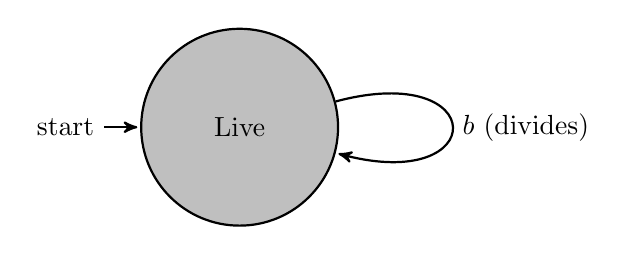
\begin{tikzpicture}[->,>=stealth',shorten >=1pt,auto,node distance=4cm,thick]
\tikzstyle{every state}=[fill=lightgray,draw=black,text=black,minimum size=2.5cm]
% \node[initial,state] (L) {Live}; 
\node[initial,state] (L) {Live}; 
\path 
(L) edge [loop right] node {$b$ (divides)} (L);
\end{tikzpicture}
% \end{centering}
\caption{The graph structure of the Live cell cycle model. The default phase is marked 
``start.''}
\label{fig:cycle_model:live}
\end{mdframed}
\end{figure}

\TOClink 

\subsubsection{Ki-67 Basic (\texttt{Ki67\_basic})\\
(Code: \texttt{PhysiCell\_constants::basic\_Ki67\_cycle\_model})}
\label{sec:Standard_Models:Ki67_Basic}
This \v|Cycle_Mode| has the following \v|Phase|s: 
\begin{enumerate}
\item 
\textbf{Phase 0:} Named \v|Ki67-| with code \v|PhysiCell_constants::Ki67_negative|. 

\item 
\textbf{Phase 1:} Named \v|Ki67+| with code \v|PhysiCell_constants::Ki67_positive|. 
\end{enumerate}

In this model, Ki67- cells (those staining negative for the 
cell proliferation marker Ki67) can enter the cell cycle to 
become Ki67+ cells, at transition rate $r_{01}$. Ki67+ cells 
divide into two Ki67- cells at rate $r_{10}$. 
See Fig. \ref{fig:cycle_model:ki67_basic}. The 
population-scale model is given by: 
\beqa
\frac{d\t{Ki67-}}{dt} & = & -r_{01} \t{Ki67-} + 2 r_{10} \t{Ki67+} \\
\frac{d\t{Ki67+}}{dt} & = &  r_{01} \t{Ki67-} -r_{10} \t{Ki67+} 
\eeqa
Further details on the \emph{biology} of this model (including 
details the placement of daughter cells and changes in cell 
volume) and reference parameter values can be found in \cite{ref:PhysiCell}. 

\begin{figure}
\begin{mdframed}[style=mystyle]
% \begin{centering}
% \begin{tikzpicture}
% \tikzset{vertex/.style = {shape=circle,draw,minimum size=1cm}}
% \tikzset{edge/.style = {->,> = latex'}}
% vertices
% \node[vertex] (L) at (0,0) {Live};
%edges
% \draw[edge] (L) to[loop right] (L) {};
% \end{tikzpicture}
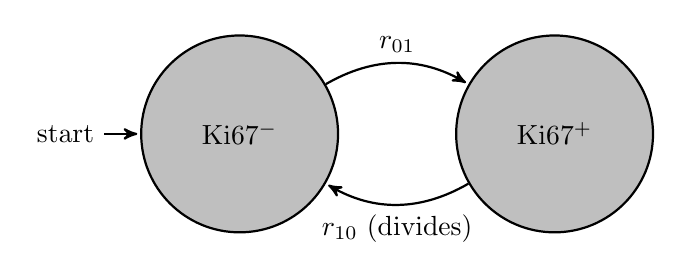
\begin{tikzpicture}[->,>=stealth',shorten >=1pt,auto,node distance=4cm,thick]
\tikzstyle{every state}=[fill=lightgray,draw=black,text=black,minimum size=2.5cm]
% \node[initial,state] (L) {Live}; 
\node[initial,state] (A) {Ki67$^-$}; 
\node[state] (B) [right of=A]{Ki67$^+$}; 
\path 
(A) edge [bend left] node {$r_{01}$} (B)
(B) edge [bend left] node {$r_{10}$ (divides)} (A);
\end{tikzpicture}
% \end{centering}
\caption{The graph structure of the Ki67 Basic cell cycle model. The default phase is marked 
``start.''}
\label{fig:cycle_model:ki67_basic}
\end{mdframed}
\end{figure}

\TOClink 

\subsubsection{Ki-67 Advanced (\texttt{Ki67\_advanced})\\
(code: \texttt{PhysiCell\_constants::advanced\_Ki67\_cycle\_model})}
\label{sec:Standard_Models:Ki67_Advanced}
This \v|Cycle_Mode| has the following \v|Phase|s: 
\begin{enumerate}
\item 
\textbf{Phase 0:} Named \v|Ki67-| with code \v|PhysiCell_constants::Ki67_negative|. This is the default 
phase of the model. 

\item 
\textbf{Phase 1:} Named \v|Ki67+ (premitotic)| with code \\ \v|PhysiCell_constants::Ki67_positive_premitotic|. 

\item 
\textbf{Phase 2:} Named \v|Ki67+ (postmitotic)| with code \\ \v|PhysiCell_constants::Ki67_positive_postmitotic|. 

\end{enumerate}

In this model, Ki67- cells (those staining negative for the 
cell proliferation marker Ki67) can enter the cell cycle to 
become premitotic Ki67+ cells, at transition rate $r_{01}$. Ki67+ premitotic cells 
divide into two Ki67+ postmitotic cells at rate $r_{12}$. 
Postmitotic Ki67+ cells become Ki67- cells at rate $r_{20}$. 
See Fig. \ref{fig:cycle_model:ki67_advanced}. The 
population-scale model is given by: 
\beqa
\frac{d\t{Ki67-}}{dt} & = & -r_{01} \t{Ki67-} + r_{10} \t{Ki67+ (post)} \\
\frac{d\t{Ki67+ (pre)}}{dt} & = &  r_{01} \t{Ki67-} -r_{12} \t{Ki67+ (pre)} \\
\frac{d\t{Ki67+ (post)}}{dt} & = &  2r_{12} \t{Ki67+ (pre)} -r_{20} \t{Ki67+ (post)} 
\eeqa
Further details on the \emph{biology} of this model (including 
details the placement of daughter cells and changes in cell 
volume) and reference parameter values can be found in \cite{ref:PhysiCell}. 

\begin{figure}
\begin{mdframed}[style=mystyle]
% \begin{centering}
% \begin{tikzpicture}
% \tikzset{vertex/.style = {shape=circle,draw,minimum size=1cm}}
% \tikzset{edge/.style = {->,> = latex'}}
% vertices
% \node[vertex] (L) at (0,0) {Live};
%edges
% \draw[edge] (L) to[loop right] (L) {};
% \end{tikzpicture}
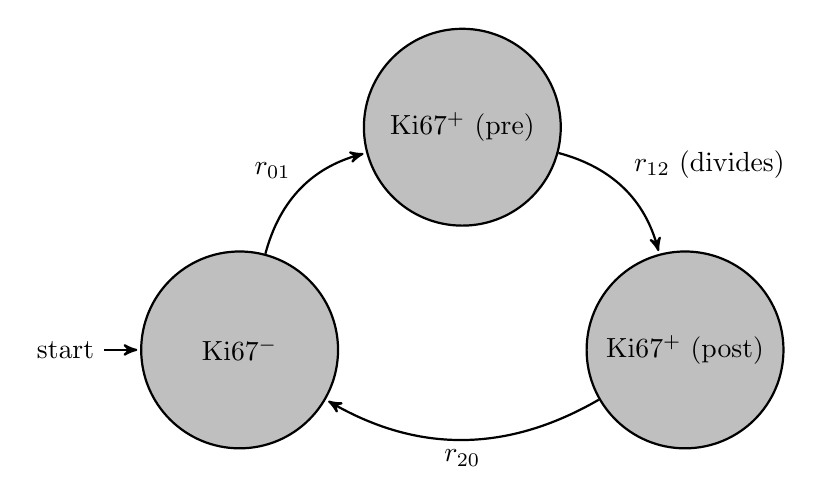
\begin{tikzpicture}[->,>=stealth',shorten >=1pt,auto,node distance=4cm,thick]
\tikzstyle{every state}=[fill=lightgray,draw=black,text=black,minimum size=2.5cm]
% \node[initial,state] (L) {Live}; 
\node[initial,state] (A) {Ki67$^-$}; 
\node[state] (B) [above right of=A]{Ki67$^+$ (pre)}; 
\node[state] (C) [below right of=B]{Ki67$^+$ (post)}; 
\path 
(A) edge [bend left] node {$r_{01}$} (B)
(B) edge [bend left] node {$r_{12}$ (divides)} (C)
(C) edge [bend left] node {$r_{20}$} (A);
\end{tikzpicture}
\caption{The graph structure of the Ki67 Advanced cell cycle model. The default phase is marked 
``start.''}
\label{fig:cycle_model:ki67_advanced}
\end{mdframed}
\end{figure}

\TOClink 

\subsubsection{Flow Cytometry (\texttt{flow\_cytometry\_cycle\_model})\\
(code: \texttt{PhysiCell\_constants::flow\_cytometry\_cycle\_model})}
\label{sec:Standard_Models:Flow_Cytometry}
This \v|Cycle_Mode| has the following \v|Phase|s: 
\begin{enumerate}
\item 
\textbf{Phase 0:} Named \v|G0G1| with code \v|PhysiCell_constants::G0G1_phase|. This is the default 
phase of the model. 

\item 
\textbf{Phase 1:} Named \v|S| with code \\ \v|PhysiCell_constants::S_phase|. 

\item 
\textbf{Phase 2:} Named \v|G2M| with code \\ \v|PhysiCell_constants::G2M_phase|. 

\end{enumerate}

In this model, $G_0/G_1$ cells can enter the cell cycle to 
become $S$-phase cells, at transition rate $r_{01}$. $S$-phase cells 
can become $G_2/M$-phase cells at rate $r_{12}$. 
$G_2/M$-phase cells can divide into two $G_0/G_1$ daughter cells 
at rate $r_{20}$. 
See Fig. \ref{fig:cycle_model:flow_cytometry}. The 
population-scale model is given by: 
\beqa
\frac{d\t{G0G1}}{dt} & = & -r_{01} \t{G0G1} + 2 r_{20} \t{G2M} \\
\frac{d\t{S}}{dt} & = &  r_{01} \t{G0G1} -r_{12} \t{S} \\
\frac{d\t{G2M}}{dt} & = &  r_{12} \t{S} -r_{20} \t{G2M} 
\eeqa
Further details on the \emph{biology} of this model (including 
details the placement of daughter cells and changes in cell 
volume) and reference parameter values can be found in \cite{ref:PhysiCell}. 

\begin{figure}
\begin{mdframed}[style=mystyle]
% \begin{centering}
% \begin{tikzpicture}
% \tikzset{vertex/.style = {shape=circle,draw,minimum size=1cm}}
% \tikzset{edge/.style = {->,> = latex'}}
% vertices
% \node[vertex] (L) at (0,0) {Live};
%edges
% \draw[edge] (L) to[loop right] (L) {};
% \end{tikzpicture}
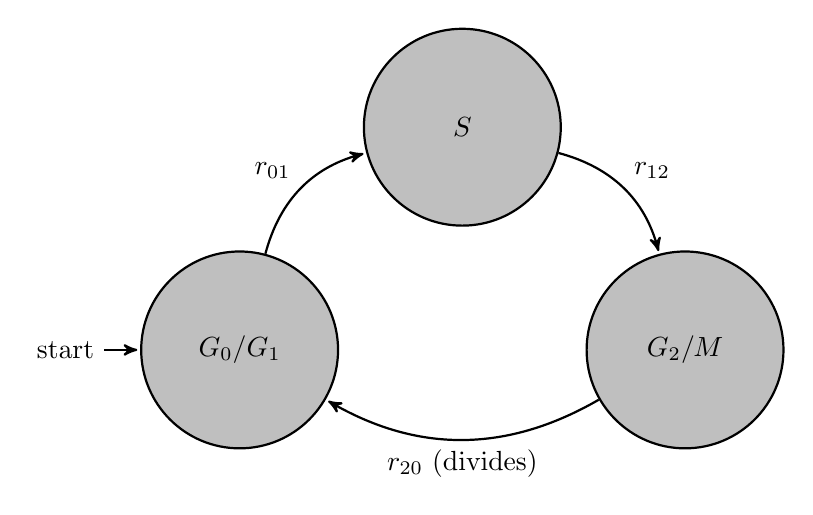
\begin{tikzpicture}[->,>=stealth',shorten >=1pt,auto,node distance=4cm,thick]
\tikzstyle{every state}=[fill=lightgray,draw=black,text=black,minimum size=2.5cm]
% \node[initial,state] (L) {Live}; 
\node[initial,state] (A) {$G_0/G_1$}; 
\node[state] (B) [above right of=A]{$S$}; 
\node[state] (C) [below right of=B]{$G_2/M$}; 
\path 
(A) edge [bend left] node {$r_{01}$} (B)
(B) edge [bend left] node {$r_{12}$ } (C)
(C) edge [bend left] node {$r_{20}$ (divides)} (A);
\end{tikzpicture}
\caption{The graph structure of the Flow Cytometry cell cycle model. The default phase is marked 
``start.''}
\label{fig:cycle_model:flow_cytometry}
\end{mdframed}
\end{figure}

\TOClink 


\subsubsection{Flow Cytometry Separated (\texttt{flow\_cytometry\_separated\_cycle\_model})\\
(code: \texttt{PhysiCell\_constants::flow\_cytometry\_separated\_cycle\_model})}
\label{sec:Standard_Models:Flow_Cytometry_Separated}
This \v|Cycle_Mode| has the following \v|Phase|s: 
\begin{enumerate}
\item 
\textbf{Phase 0:} Named \v|G0G1| with code \v|PhysiCell_constants::G0G1_phase|. This is the default 
phase of the model. 

\item 
\textbf{Phase 1:} Named \v|S| with code \\ \v|PhysiCell_constants::S_phase|. 

\item 
\textbf{Phase 2:} Named \v|G2| with code \\ \v|PhysiCell_constants::G2_phase|. 

\item 
\textbf{Phase 3:} Named \v|M| with code \\ \v|PhysiCell_constants::M_phase|. 

\end{enumerate}

In this model, $G_0/G_1$ cells can enter the cell cycle to 
become $S$-phase cells, at transition rate $r_{01}$. $S$-phase cells 
can become $G_2$-phase cells at rate $r_{12}$. 
$G_2$-phase cells can become $M$-phase cells at rate $r_{23}$. 
$M$-phase cells can divide into two $G_0/G_1$ daughter cells 
at rate $r_{30}$. 
See Fig. \ref{fig:cycle_model:flow_cytometry_separated}. The 
population-scale model is given by: 
\beqa
\frac{d\t{G0G1}}{dt} & = & -r_{01} \t{G0G1} + 2 r_{30} \t{M} \\
\frac{d\t{S}}{dt} & = &  r_{01} \t{G0G1} -r_{12} \t{S} \\
\frac{d\t{G2}}{dt} & = &  r_{12} \t{S} -r_{23} \t{G2} \\
\frac{d\t{M}}{dt} & = &  r_{23} \t{G2} -r_{30} \t{M} 
\eeqa
Further details on the \emph{biology} of this model (including 
details the placement of daughter cells and changes in cell 
volume) and reference parameter values can be found in \cite{ref:PhysiCell}. 

\begin{figure}
\begin{mdframed}[style=mystyle]
% \begin{centering}
% \begin{tikzpicture}
% \tikzset{vertex/.style = {shape=circle,draw,minimum size=1cm}}
% \tikzset{edge/.style = {->,> = latex'}}
% vertices
% \node[vertex] (L) at (0,0) {Live};
%edges
% \draw[edge] (L) to[loop right] (L) {};
% \end{tikzpicture}
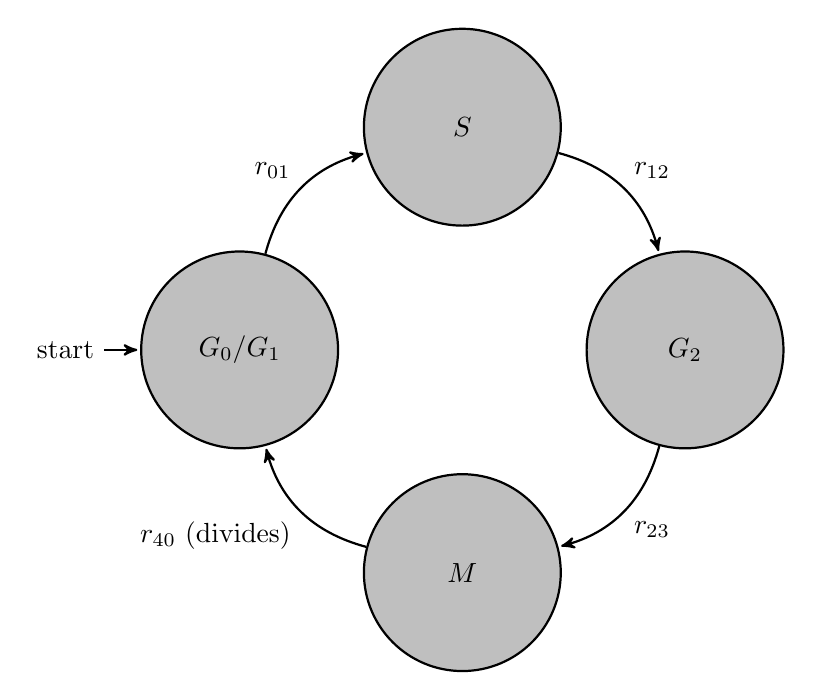
\begin{tikzpicture}[->,>=stealth',shorten >=1pt,auto,node distance=4cm,thick]
\tikzstyle{every state}=[fill=lightgray,draw=black,text=black,minimum size=2.5cm]
% \node[initial,state] (L) {Live}; 
\node[initial,state] (A) {$G_0/G_1$}; 
\node[state] (B) [above right of=A]{$S$}; 
\node[state] (C) [below right of=B]{$G_2$}; 
\node[state] (D) [below left of=C]{$M$}; 
\path 
(A) edge [bend left] node {$r_{01}$} (B)
(B) edge [bend left] node {$r_{12}$ } (C)
(C) edge [bend left] node {$r_{23}$ } (D)
(D) edge [bend left] node {$r_{40}$ (divides)} (A);
\end{tikzpicture}
\caption{The graph structure of the Flow Cytometry Separated cell cycle model. The default phase is marked 
``start.''}
\label{fig:cycle_model:flow_cytometry_separated}
\end{mdframed}
\end{figure}

\TOClink 







\subsection{Death Cycle Models}
\label{sec:Standard_Models:Death}
PhysiCell currently includes two pre-built death cycle models. More models 
may be added in future releases, such as autophagy. 

\subsubsection{Apoptosis (\texttt{apoptosis})\\
(code: \texttt{PhysiCell\_constants::apoptosis\_death\_model})}
\label{sec:Standard_Models:Apoptosis}
This \v|Cycle_Mode| has the following \v|Phase|s: 
\begin{enumerate}
\item 
\textbf{Phase 0:} Named \v|Apoptotic| with code \v|PhysiCell_constants::apoptotic|. 
\end{enumerate}
In this model, apoptotic cells shrink and exit the phase at 
rate $r_{01}$ (with fixed duration $1 / r_{01}$). Cells are removed 
from the simulation at the end of the apoptotic phase. 
(PhysiCell currently uses a dummy ``debris'' phase to avoid coding a 
phase transition from the apoptotic phase to the apoptotic phase; this 
may be removed in future releases.) 
See Fig. \ref{fig:death_model:apoptosis}. The 
population-scale model is given by: 
\beq
\frac{d\t{Apoptotic}}{dt} = -r_{01} \t{Apoptotic}. 
\eeq
Further details on the \emph{biology} of this model (including 
details on changes in cell volume) and reference parameter values can be found in \cite{ref:PhysiCell}. 
% Please note that the debris phase is a computational convenience (to avoid 
% requiring a phase transition from the apoptotic phase to the apoptotic phase), but 
% it may be removed in future PhysiCell releases. Cells do not actually 
% enter this state in this model. 

\begin{figure}
\begin{mdframed}[style=mystyle]
\begin{tikzpicture}[->,>=stealth',shorten >=1pt,auto,node distance=5.5cm,thick]
\tikzstyle{every state}=[fill=lightgray,draw=black,text=black,minimum size=3cm]
\node[initial,state] (A) {Apoptotic}; 
\node [state] (end) [right of=A, node distance=5.5cm,fill=none,draw=none]{removed};
\path (L) edge node {$r_{01}$} (end); 
\end{tikzpicture}
\caption{The graph structure of the Apoptosis death cycle model. The default phase is marked 
``start,'' and the cell is removed as marked.`}
\label{fig:death_model:apoptosis}
\end{mdframed}
\end{figure}

\TOClink 


\subsubsection{Necrosis (\texttt{necrosis})\\
(code: \texttt{PhysiCell\_constants::necrosis\_death\_model})}
\label{sec:Standard_Models:Necrosis}
This \v|Cycle_Mode| has the following \v|Phase|s: 
\begin{enumerate}
\item 
\textbf{Phase 0:} Named \v|Necrotic (swelling)| with code \v|PhysiCell_constants::necrotic_swelling|. 
\item
\textbf{Phase 1:} Named \v|Necrotic (lysed)| with code \v|PhysiCell_constants::necrotic_lysed|. 
\end{enumerate}
In this model, unlysed necrotic cells swell and attempt to 
transition to the lysed necrotic  phase. There is a block on the 
transition until the cell reaches a sufficient 
total volume. Lysed cells gradually shrink (and calcify, if 
enable) and exit the phase at 
rate $r_{12}$. Cells are removed 
from the simulation at the end of the lysed necrotic phase. 
(PhysiCell currently uses a dummy ``debris'' phase to avoid coding a 
phase transition from the lysed necrotic phase phase to another necrotic phase; 
this may be removed in future releases.) 
See Fig. \ref{fig:death_model:necrosis}. 

Further details on the \emph{biology} of this model (including 
details on changes in cell volume) and reference parameter values can be found in \cite{ref:PhysiCell}. 

% Please note that the debris phase is a computational convenience (to avoid 
% requiring a phase transition from the apoptotic phase to the apoptotic phase), but 
% it may be removed in future PhysiCell releases. Cells do not actually 
% enter this state in this model. 

\begin{figure}
\begin{mdframed}[style=mystyle]
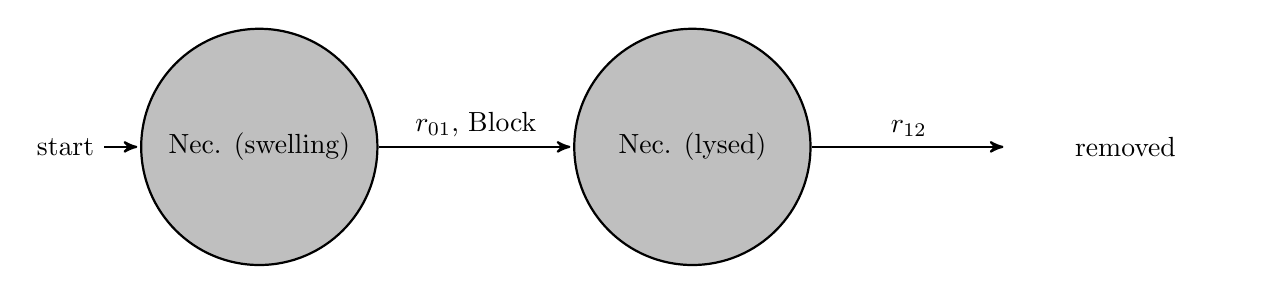
\begin{tikzpicture}[->,>=stealth',shorten >=1pt,auto,node distance=5.5cm,thick]
\tikzstyle{every state}=[fill=lightgray,draw=black,text=black,minimum size=3cm]
\node[initial,state] (S) {Nec. (swelling)}; 
\node[state] (L) [right of=S]{Nec. (lysed)}; 
\node [state] (end) [right of=L, node distance=5.5cm,fill=none,draw=none]{removed};
\path 
(S) edge node {$r_{01}$, Block} (L) 
(L) edge node {$r_{12}$} (end); 
\end{tikzpicture}
\caption{The graph structure of the Necrosis death cycle model. The default phase is marked 
``start,'' and the cell is removed as marked. The transition from the 
unlysed to lysed state is blocked until the cell volume reaches sufficient volume.}
\label{fig:death_model:necrosis}
\end{mdframed}
\end{figure}

\TOClink 

\subsection{Volume model (\texttt{standard\_volume\_update\_function})}
\label{sec:Standard_Models:Volume}
The standard volume model separately evolves the total fluid volume, 
cytoplasmic solid volume, and nuclear solid volume, as a system of ODEs 
(given in \cite{ref:PhysiCell}). The standard model also updates 
cell calcification (but the default rate parameter is zero). 
% \begin{eqnarray*}
% \frac{d}{dt}\tt{volume.fluid} 
% & = & 
% \tt{volume.fluid\_change\_rate} \cdot \nonumber \\
% && 
% \Bigl( 
% \tt{volume.target\_fluid\_fraction}
% \tt{volume.total} - \tt{volume.fluid} \Bigr) \\
%
% \tt{volume.nuclear\_fluid}
% & = & \frac{ \tt{volume.nuclear} }{ \tt{volume.total} }
% \cdot \tt{volume.fluid} \\
%
% \tt{volume.cytoplasmic\_fluid} & = & 
% \tt{volume.fluid} - \tt{volume.nuclear\_fluid} \\
%
% \frac{d}{dt} 
% \tt{volume.nuclear\_solid} 
% & = & 
% \tt{volume.nuclear\_biomass\_change\_rate} \cdot \nonumber \\
% && 
% \Bigl( 
% \tt{volume.target\_solid\_nuclear} - 
% \tt{volume.nuclear\_solid}
% \Bigr) \\
%
% \tt{volume.target\_solid\_cytoplasmic} 
% & = & 
% \tt{volume.target\_cytoplasmic\_to\_nuclear\_ratio} 
% \cdot \nonumber \\
% &&
% \tt{volume.target\_solid\_nuclear} \\
%
% \frac{d}{dt} 
% \tt{volume.cytoplasmic\_solid}
% & = & 
% \Bigl( 
% \tt{volume.target\_solid\_cytoplasmic} - 
% \tt{volume.cytoplasmic\_solid}
% \Bigr)
% \end{eqnarray*}
See Section \ref{sec:Volume} for more information on the \v|Volume| class 
in the \v|Phenotype|, and \cite{ref:PhysiCell} for the biological 
details of this model. 
\TOClink 

\subsection{Cell velocity model (\texttt{standard\_update\_cell\_velocity})}
\label{sec:Standard_Models:Velocity}
In this model, the cell uses the mechanics interaction 
data structure to find nearby cells, adds the contributions 
from adhesion and ``repulsion,'', adds the effects of 
basement membrane interactions 
(by calling \v|functions.add_cell_basement_membrane_interactions|), 
then computes the contribution to cell velocity by the motility 
model (by calling \v|update_motility_vector|, 
which in turn calls \\
\v|functions.update_migration_bias|). 
See Section \ref{sec:Motility} for details on motility,
Section \ref{sec:Mechanics} for key cell mechanics phenotype 
parameters, and Section \ref{sec:Cells} for more information 
on Cells and their member functions. 

\TOClink 

\subsection{Up orientation model (\texttt{up\_orientation})}
\label{sec:Standard_Models:Orientation}
By default 3-D cells have no preferred orientation, and 2-D cells 
have an ``up'' orientation (set to [0,0,1]) to ensure they stay 
in the $z=0$ plane. This supplied function is 
\v|up_orientation|. 

\subsection{Oxygen-dependent phenotype \\
(\texttt{update\_cell\_and\_death\_parameters\_O2\_based})}
\label{sec:Standard_Models:Microenvironment_Phenotype}
Oxygen-dependent cell proliferation and death rates are so commonly 
needed in cancer models that we include a model function 
as standard: 
\v|update_cell_and_death_parameters_O2_based|. Here is the 
overall model for proliferation: 

\begin{enumerate}
\item 
Sample the microenvironment for the oxygen concentration 
$\sigma$ at the 
cell center. 
\item 
If $\sigma \ge \tt{parameters.o2\_proliferation\_saturation}$, 
then the cycle entry rate is set to 100\% of the entry rate 
in the \v|pReference_live_phenotype| reference phenotype. 

\item 
If $\sigma \le \tt{parameters.o2\_proliferation\_threshold}$, 
then the cycle entry rate is set to 0\% of the entry rate 
in the \v|pReference_live_phenotype| reference phenotype. 

\item 
Otherwise, the reference cycle entry rate is scaled by 
\beq
\frac{ \sigma - 
\tt{parameters.o2\_proliferation\_threshold} }
{ \tt{parameters.o2\_proliferation\_saturation} - 
\tt{parameters.o2\_proliferation\_threshold} }
\eeq

\end{enumerate}

% This function currently works for the following 
% cell cycle models: 
%
% \begin{enumerate}
% \item 
% The Ki67 advanced model 
% (\v|PhysiCell_constants::advanced_Ki67_cycle_model|). See 
% Section \ref{sec:Standard_Models:Ki67_Advanced}. 
%
% \item 
% The Ki67 basic model 
% (\v|PhysiCell_constants::basic_Ki67_cycle_model|). See 
% Section \ref{sec:Standard_Models:Ki67_Basic}. 
%
% \item 
% The Live model 
% (\v|PhysiCell_constants::live_cells_cycle_model|). See 
% Section \ref{sec:Standard_Models:Ki67_Live}. 
% \end{enumerate}

Here is the overall model for the necrosis death rate: 
\begin{enumerate}
\item 
Sample the microenvironment for the oxygen concentration 
$\sigma$ at the 
cell center. 
\item 
If $\sigma \ge \tt{parameters.o2\_necrosis\_threshold}$, 
then the necrotic death rate is zero. 

\item 
If $\sigma \le \tt{parameters.o2\_necrosis\_max}$, 
then the necrosis death rate is set to 100\% of \\
\v|parameters.max_necrosis_rate|. 

\item 
Otherwise, the necrotic death rate is scaled by 
\beq
\frac{ \tt{parameters.o2\_necrosis\_threshold} - \sigma }
{\tt{parameters.o2\_necrosis\_threshold} - \tt{parameters.o2\_necrosis\_max} }
\eeq
\end{enumerate}

This function currently works for the following 
cell cycle models: 

\begin{enumerate}
\item 
The Ki67 advanced model 
(\v|PhysiCell_constants::advanced_Ki67_cycle_model|). See 
Section \ref{sec:Standard_Models:Ki67_Advanced}. 

\item 
The Ki67 basic model 
(\v|PhysiCell_constants::basic_Ki67_cycle_model|). See 
Section \ref{sec:Standard_Models:Ki67_Basic}. 

\item 
The Live model 
(\v|PhysiCell_constants::live_cells_cycle_model|). See 
Section \ref{sec:Standard_Models:Live}. 
\end{enumerate}

See Section \ref{sec:Cycle} for more on the cell cycle portion 
of the phenotype, Section ref{sec:Death} for more information 
on the death phenotype elements, 
Section \ref{sec:Standard_Models:Death} on standard death models, and  
Section \ref{sec:Standard_Models:Cycle} on standard cell cycle models. 
See \cite{ref:PhysiCell} for more on the biology of these 
models. 

\TOClink 

\section{Examples}
\label{sec:Examples}

\subsection{Working with \texttt{Cell} functions}

\subsubsection{Example: a custom volume model}
\label{sec:Examples:volume_model}
Here, we will define a simpler volume model that only 
upates the total volume. We 
use the mathematical model: 
\beq
\frac{d}{dt} 
\tt{volume.total} = r \left( V^* - \tt{volume.total} \right),  
\eeq
where 
\beqa
V^* & = & \left( \frac{1 + \tt{target\_cytoplasmic\_to\_nuclear\_ratio}}
{1 - \tt{volume.fluid\_fraction}} \right) \cdot 
\tt{volume.target\_solid\_nuclear} \\
r & = & 
\ln\left( 
\frac{1 - 0.95}{0.5}
\right) \tt{phenotype.cycle.model.transition\_rate(0,0)} 
\eeqa
(This uses the built-in phenotype to get the ``target'' total volume in 
terms of the built-in  targets, and it sets $r$ so that a divided cell reaches 
95\% of its target within the mean duration of the cell's interdivision 
time.) 
\begin{verbatim}
void simple_volume_function( Cell* pCell, Phenotype& phenotype, double dt )
{
    double V_target = phenotype.volume.target_solid_nuclear * 
        (1.0 + phenotype.volume.target_cytoplasmic_to_nuclear_ratio) / 
        (1-phenotype.volume.fluid_fraction); 
    double rate = phenotype.cycle.model().transition_rate(0,0) * log(0.1); 
    
    double addme = V_target; 
    addme -= phenotype.volume.total; 
    addme *= rate; 
    addme *= dt; // dt*rate*( V_target - V )
    
    phenotype.volume.total += addme; 
    
    return; 
}
\end{verbatim}

\TOClink 

\subsubsection{Example: a custom migration bias}
\label{sec:Examples:migration}
In this example, cells migrate along oxygen gradients. The 
migration speed is fastest in regions of low oxygen, 
and the migration is least stochastic (most biased) 
as the oxygenation increases. 
\begin{verbatim}
void chemotaxis_bias_function( Cell* pCell, Phenotype& phenotype , double dt )
{
    // quickly find O2 
    static int O2_index = microenvironment.find_density_index( "oxygen" ); 
    
    // sample O2 
    double o2 = pCell->nearest_density_vector()[O2_index]; 
    
    // set direction along O2 gradients 
    phenotype.motility.migration_bias_direction = pCell->nearest_gradient(O2_index); 
    normalize( &( phenotype.motility.migration_bias_direction ) ); 
    
    // set speed proportional to O2, scaled by normoxic O2 ( 160 mmHg); 
    // with a maximum of 1.2 micron per minute 
    double theta = o2 / 160.0;
    phenotype.motility.migration_speed = 1.2*(1.0-theta);   
    if( phenotype.motility.migration_speed > 1.2 )
    { phenotype.motility.migration_speed = 1.2; } 

    // the greater the oxygen, the more biased the motion 
    phenotype.motility.migration_bias = theta; 
    
    return; 
}
\end{verbatim}

\TOClink 

\subsubsection{Example: a custom cell rule}
\label{sec:Examples:custom_rule}
In this example, an immune cell tests nearby cells 
first for contact, and then for expression of an antigen (a custom variable). 
The immune cell initiates apoptosis in the target cell with 
probability that scales with the antigen expression. 
\begin{verbatim}
void immune_cell_rule( Cell* pCell, Phenotype& phenotype, double dt )
{
    static int antigen_index = 
        pCell->custom_data.find_variable_index( "antigen" ); 
    static int activation_index = 
        pCell->custom_data.find_variable_index( "activation" ); 
    
    static int apoptosis_model_index = 
        pCell->phenotype.death.find_death_model_index( "apoptosis" ); 
    
    // exit if immune function is not yet stimulated, or dead  
    if( pCell->custom_data[activation_index] < 1e-3 
        || pCell->phenotype.death.dead == true )
    { return; }

    std::vector<Cell*> nearby = pCell->cells_in_my_container(); 
    
    // test antigen on nearby cells. stop if you find one 
    // Don't try to kill dead cells. 
    // Don't kill yourself 
    Cell* pC = NULL; 
    bool stop = false; 
    int i=0; 
    
    while( !stop && i < nearby.size() )
    {
        pC = nearby[i]; 
        if( pC->custom_data[antigen_index] > 1e-3 && 
            pC->phenotype.death.dead == false && 
            pC != pCell )
        { stop = true; } 
        i++; 
        if( stop == false )
        { pC = NULL; }
    }
    
    // if we found a cell, attempt to kill it 
    if( pC )
    {
        double probability = 1.0; // dt*pC->custom_data[antigen_index]; 
        if( UniformRandom() < probability )
        {
            std::cout << "death!" << std::endl; 
            system("pause"); 
            pC->start_death( apoptosis_model_index ); 
        }
    }
    return; 
}
\end{verbatim}
Here is the code to add the custom variables to a specific cell: 
\begin{verbatim}
pCell->custom_data.add_variable( "antigen", "dimensionless", 0.0 ); 
pCell->custom_data.add_variable( "activation", "dimensionless", 0.0 ); 
\end{verbatim}
Better still, you could make cell definitions for tumor cells and 
immune cells: 
\begin{verbatim}
Cell_Definition immune_cell; 

// operations to define this type 

immune_cell.functions.custom_cell_rule = immune_cell_rule;
immune_cell.custom_data.add_variable( "activation", "dimensionless", 0.0 );

Cell_Definition MCF7 = cell_defaults; 
MCF7.custom_data.add_variable( "antigen", "dimensionless", 0.0 );
\end{verbatim}

\TOClink 

\subsubsection{Example: a custom phenotype update function}
\label{sec:Examples:phenotype_rule}
Let's create a custom phenotype update rule that uses the 
the standard oxygen-based cell birth and death rates, but 
also increases cell motility and decreases cell-cel adhesion 
in low oxygen conditions. 

Note that these effects gradually turn on and then saturate 
based on oxygen values in the cell's \v|parameters|, 
and we use the cell's \v|pReference_live_phenotype|.  
\begin{verbatim}
void custom_o2_phenotype_rule( Cell* pCell, Phenotype& phenotype, double dt )
{
   // don't bother if you're dead
   if( pCell->phenotype.death.dead == true )
   { return; }
   
   // first, call the standard function
   update_cell_and_death_parameters_O2_based(pCell,phenotype,dt);     
    
   // next, let's evaluate the oxygen 
   static int o2_index = microenvironment.find_density_index("oxygen"); 
   
   double o2 = pCell->nearest_density_vector()[o2_index];
    
   if( o2 > pCell->parameters.o2_hypoxic_response )
   { return; }
    
   // interpolation variable 
   double theta = ( pCell->parameters.o2_hypoxic_response  - o2 )/
      (pCell->parameters.o2_hypoxic_response - pCell->parameters.o2_hypoxic_saturation); 
   if( theta > 1.0 )
   { theta = 1.0; } 
    
   // increase the speed of motiltiy up to a max of 1.5 micron/min 
   phenotype.motility.is_motile = true; 
   phenotype.motility.migration_speed = 1.5; 
   phenotype.motility.migration_speed *= theta;  

   phenotype.mechanics.cell_cell_adhesion_strength = (1.0-theta);
   phenotype.mechanics.cell_cell_adhesion_strength *= 
      pCell->parameters.pReference_live_phenotype->mechanics.cell_cell_adhesion_strength;
   return; 
}
\end{verbatim}
\TOClink 

\subsubsection{Example: a custom velocity update function}
We'll add an example soon. For now, use the default, along with the 
default motility functions (which allow considerable customization!). 

\subsubsection{Example: analytical basement membrane functions}
This space held in reserve. 

\subsubsection{Example: a custom cell orientation function}
This space held in reserve. 

\subsection{Cell cycle models}

\subsubsection{Creating a custom cell cycle model}
\label{sec:Examples:custom_cell_cycle}
Let's create a simple cycle model, with three phases: Red, Green, and Blue. 
Red cells become Green. Green cells become Blue. Blue cells divide into two 
Red cells. Here's how we accomplish this using the \v|Cycle_Model| class. 
Notice that we're saving the indices of the newly-created phases for 
easier reference. 

\begin{verbatim}
Cycle_Model model;

// set up name information 
model.code = PhysiCell_constants::custom_cycle_model;
mode.name = "Red Green Blue"; 

// add the phases 
int red_index = model.add_phase( 0 , "Red" ); 
int green_index = model.add_phase( 1 , "Green" ); 
int blue_index = model.add_phase( 2 , "Blue" ); 

// set the Blue phase to have division at its end 
model.phases[blue_index].division_at_phase_exit = true; 

// set up the phase links 
model.add_phase_link( red_index , green_index , NULL ); // red -> green
model.add_phase_link( green_index , blue_index , NULL ); // green -> blue
model.add_phase_link( blue_index , red_index , NULL ); // blue -> red 

// set the transition rates
model.transition_rate(red_index,green_index) = 1.0/( 60.0 * 5.0 ); 
     // mean duration: 5 hours
model.transition_rate(green_index,blue_index) = 1.0/( 60.0 * 8.0 ); 
     // mean duration: 8 hours
model.transition_rate(blue_index,red_index) = 1.0/( 60.0 * 2.0 ); 
     // mean duration: 2 hours

// display the model 
model.display( std::cout ); 
\end{verbatim}
And this is how we would register that model in a cell definition:
\begin{verbatim}
immune_cell.phenotype.cycle.sync_to_cycle_model( rgb_model ); 
\end{verbatim}
Or in a single cell: 
\begin{verbatim}
pCell->phenotype.cycle.sync_to_cycle_model( rgb_model ); 
\end{verbatim}

\TOClink 

\subsubsection{Adding an arrest function}
\label{sec:Examples:arrest}
Suppose now that we only want to allow Blue cells to proceed to Red and divide if 
they have a fluid fraction over 50\%. (See Section \ref{sec:Volume}.) 
Then we can define an arrest function:
\begin{verbatim}
bool fluid_arrest_function(  Cell* pCell, Phenotype& phenotype, double dt )
{
     if( phenotype.volume.fluid_fraction < 0.5 )
     { return true; }
     return false; 
}
\end{verbatim}
We then assign this arrest function to the transition from the Blue phase to the Red phase: 
\begin{verbatim}
rgb_model.phase_link(blue_index,red_index).arrest_function = fluid_arrest_function; 
\end{verbatim}

\TOClink

\subsubsection{Adding a custom phase entry function}
\label{sec:Examples:phase_entry}
Suppose now that we want the cell to ``mutate'' its transition rates whenever it re-enters 
the Red phase. We can do this with an entry function: 
\begin{verbatim}
void my_mutation_function( Cell* pCell, Phenotype& phenotype, double dt )
{
     // mutate all transition rates by a uniformly-distributed 
     // number within 10\% of the current value
     double multiplier = 0.9 + 0.2*uniform_random(); 
     phenotype.cycle.data.transition_rate(0,1) *= multiplier; 

     multiplier = 0.9 + 0.2*uniform_random(); 
     phenotype.cycle.data.transition_rate(1,2) *= multiplier; 

     multiplier = 0.9 + 0.2*uniform_random(); 
     phenotype.cycle.data.transition_rate(2,0) *= multiplier; 

     return; 
}
\end{verbatim}

Then, we assign this as the entry function for the Red phase: 
\begin{verbatim}
rgb_model.phases[red_index].entry_function = my_mutation_function; 
\end{verbatim}

Alternatively, we can assign this as the exit function for the Blue-Red transition: 
\begin{verbatim}
rgb_model.phase_link(blue_index,red_index).exit_function = my_mutation_function; 
\end{verbatim}
\TOClink 

% \pagebreak \pagebreak 

\section{Future}
\label{sec:Future_Plans}
Several features are planned for upcoming PhysiCell releases: 
\begin{enumerate}
\item 
We will further refine the MultiCellDS output functions to capture 
more of the cell's state, including custom variable values. 
\red{(Completed in Version 1.2.2)}

\item 
We will add functions to read in a saved simulation state. 

\item 
We will add an XML-based configuration file. 
\red{(Completed in Version 1.3.0)}

\item 
We will add a function like 
\v|void contact_interaction_function(Cell*,Phenotype&,double)| 
to allow cell contact-based signaling and behavior changes. 

\item 
We plan to start actively tracking the cell's list of mechanically interacting neighbors in \\
\v|cell.state.neighbors|

\item 
We will further develop \v|cell.state.simple_pressure| and provide better examples. 

\item
We will create a standard \v|standard_update_orientation| function to 
let cells rotate towards a preferred orientation (which will be based upon 
its neighbors). 

\item 
We will generalize the cell-cell adhesion model to allow differing levels of adhesion 
between different types of cells. \red{(Completed in Version 1.2.0)} 

\item 
We will merge the \v|Vector_Variable| and \v|Variable| types for a more unified 
\v|Custom_Cell_Data| struture. 

\item 
We may update \v|motilty| and associated update functions to 
build in some hysteresis (bias towards the last direction of the day).

\item 
We will consider partial SBML support for importing molecular-scale models. 

\item 
We will continue to refine XML parsing for options and configuration. 

\item 
We will allow ellipsoidal cell potential functions for better approximation of cell shapes. 

\item 
We will introduce  a standard library of simplified (bulk) vasculatures. 

\item 
We will introduce a standard library of simplified ECM functions. 

\end{enumerate}

\TOClink 

% \section{Last code changes}

% \begin{enumerate}
% \item 
% Fixes from Farzin: the \v|get_total_volume| should reference phenotype volume, 
% not the basic agent. Also, have it give a warning like the email. \DONE

% \item 
% Fix the MultiCellDS function to use the correct volume! \DONE

% \item 
% Rename \v|update_migration_bias_direction| to 
% \v|update_migration_bias| to more clearly note that 
% teh speed, bias direction, and bias parameter could all be 
% updated here. \DONE 

% \item 
% Make new \v|Cell.Phenotype| or \v|Cell| functions to directly 
% trigger (and start!) apoptosis, necrosis, and arbitrary death 
% models. Model it after the 
% code I sent to Farzin. Make this at the cell level. \DONE

% \item 
% I think we ought to have cell death cut secretions to 0, and 
% uptake by one order of magnitude.  \DONE 

% \item 
% I think we ought to have a more reasonable reference value for oxygen. 
% (Is this even used?) So far, doesn't seem to be used. I think 
% for the refernce values, get something from \DONE

% \item 
% Get more reasonabler refernce apoptosis and cycling parameters for 
% MCF10A. Let reference O2 be normoxic 21\%. Fit 
% the Ki67 models after fitting the live model. \DONE 

% \item 
% topupper in the various ``find'' functions (nope!) 
% just state that its case insensitive \DONE 

% \end{enumerate}

\section{Some notes on parameter values}
% apoptosis ~ 2%:
%
% https://breast-cancer-research.biomedcentral.com/articles/10.1186/bcr949
%
% proliferation: http://clincancerres.aacrjournals.org/content/7/11/3640
% fit figure 2: r = (6*log(10) - 5*log(10))/( 24 * 5 - 24*2.5 ) ~ 0.039 
%
% NCI PDF: 16 hour doubling time: log(2)/16 ~ 0.043 
%
% Edwin's in MultiCellDS: 0.02 to 0.08 (too fast vs. too slow), 0.04 in range 
%
We chose reference proliferation and apoptosis rates for  the 
generic breast epithelium line (calibrated to MCF-10A) 
% MCF10A breast cell line 
so that the apoptotic fraction is approximately 2\% 
\cite{ref:MCF10A_apoptosis}, and the net proliferation rate 
(for the total cell population) is on the 
order of 0.04 hr${}^\textrm{-1}$ \cite{ref:MultiCellDS,ref:MCF10A-NeoST,ref:MCF10A_PSON}. 

\subsection{Live cycle model}
\label{sec:parameters:live}
For the Live cell model (Section \ref{sec:Standard_Models:Live}), we fit the 
system of ODEs
\beqa
\frac{d}{dt}\tt{Live} & = & (b-d)\tt{Live} \\
\frac{d}{dt}\tt{Apoptotic} & = & d\tt{Live} - \frac{1}{T_A} \tt{Apoptotic}, 
\eeqa
and we note that 
\beqa
\frac{d}{dt}\tt{Total} 
& = & b \tt{Live} - \frac{1}{T_A} \tt{Apoptotic} \nonumber \\ 
& = & \left( b (1-\textrm{AI}) - \frac{\textrm{AI}}{T_A} \right) \tt{Total} \nonumber \\ 
& = & r \tt{Total} 
\eeqa
Here, $r = 0.04\textrm{ hr}^{-1}$, $\textrm{AI} = 0.02$ is the apoptotic index, and
$T_A = 8.6 \textrm{ hour}$ (Section \ref{sec:Standard_Models:Apoptosis}). Thus, 
\beq
b = \frac{r + \frac{1}{T_A}\textrm{AI}}{1 - \textrm{AI}} \sim 0.0432 \textrm{ hr}^{-1}. 
\eeq
To get the death rate $d$, we use a simple iterative fitting method 
(see \\
\v|./documentation/matlab/tune_death_in_live_model|) to get $d \sim 0.00319 \textrm{ hr}^{-1}$. 

\TOClink 

\subsection{Ki67 Basic model}
\label{sec:parameters:Ki67_basic}
For the Ki67 Basic model (Section \ref{sec:Standard_Models:Ki67_Basic}), 
we fit the system of ODEs 
\beqa
\frac{d}{dt}\tt{Ki67-} & = & -\left( \frac{1}{T_Q} + d \right) \tt{Ki67-} + \frac{2}{T_K}\tt{Ki67+}  \\
\frac{d}{dt}\tt{Ki67+} & = & \frac{1}{T_Q} \tt{Ki67-} - \left( \frac{1}{T_K} + d \right) \tt{Ki67+} \\
\frac{d}{dt}\tt{Apoptotic} & = & d\left( \tt{Ki67-} + \tt{Ki67+} \right) -\frac{1}{T_A} \tt{Apoptotic}, 
\eeqa
and we note that 
\beqa
\frac{d}{dt}\tt{Total} 
& = & \frac{1}{t_K} \tt{Ki67+} - \frac{1}{T_A} \tt{Apoptotic} \nonumber \\ 
& = & \left( \frac{\textrm{KI}}{T_K} - \frac{\textrm{AI}}{T_A} \right) \tt{Total} \nonumber \\ 
& = & r \tt{Total} 
\eeqa
We set $T_K = 13 + 2.5$ hr (the duration of the two phases in the Ki67 Advanced model), 
$r = 0.04 \textrm{ hr}^{-1}$, and we set AI = 0.02 as before and keep 
$d = 0.00319 \textrm{ hr}^{-1}$ from the prior estimate. We thus need to fit  
$T_Q$. We use a simple iterative fitting method 
(see \v|./documentation/matlab/tune_Ki67_basic|) to get $T_Q \sim 4.59 \textrm{ hr}$. 

\TOClink 

\subsection{Ki67 Advanced model}
\label{sec:parameters:Ki67_advanced}
For the Ki67 Advanced model (Section \ref{sec:Standard_Models:Ki67_Advanced}), 
we fit the system of ODEs 
\beqa
\frac{d}{dt}\tt{Ki67-} & = & -\left( \frac{1}{T_Q} + d \right) \tt{Ki67-} + \frac{1}{T_{K2}}\tt{Ki67+}_2  \\
\frac{d}{dt}\tt{Ki67+}_1 & = & \frac{1}{T_Q} \tt{Ki67-} - \left( \frac{1}{T_{K1}} + d \right) \tt{Ki67+}_1 \\
\frac{d}{dt}\tt{Ki67+}_2 & = &  \frac{2}{T_{K1}} \tt{Ki67+}_1 - \left( \frac{1}{T_{K2}} + d \right) \tt{Ki67+}_2 \\
\frac{d}{dt}\tt{Apoptotic} & = & d\left( \tt{Ki67-} + \tt{Ki67+}_1 + \tt{Ki67+}_2 \right) -\frac{1}{T_A} \tt{Apoptotic}, 
\eeqa
and we note that 
\beqa
\frac{d}{dt}\tt{Total} 
& = & \frac{1}{T_{K1}} \tt{Ki67+}_1 - \frac{1}{T_A} \tt{Apoptotic} \nonumber \\ 
& = & \left( \frac{\textrm{KI}_1}{T_{K1}} - \frac{\textrm{AI}}{T_A} \right) \tt{Total} \nonumber \\ 
& = & r \tt{Total} 
\eeqa
We set $T_{K1} = 13$ hr, $T_{K2} = 2.5$ hr, $T_A = 8.6$ hr, and 
$r = 0.04 \textrm{ hr}^{-1}$, and we set AI = 0.02 as before and keep 
$d = 0.00319 \textrm{ hr}^{-1}$ from the prior estimate. We thus need to fit  
$T_Q$. We use a simple iterative fitting method 
(see \v|./documentation/matlab/tune_Ki67_advanced|) to get $T_Q \sim 3.62 \textrm{ hr}$ for this model. 
% It is interesting to note that this parameter set gives an (predicted; unfitted) Ki67+ fraction of 
% approximately 74\%, in line with independent MCF10A measurements 
% in 21\% oxygenation prior to confluence effects 
\cite{ref:Ki67_MCF10A}. 

\TOClink 

\subsection{Flow Cytometry model}
\label{sec:parameters:flow_cytometry}
For the Flow Cytometry model (Section \ref{sec:Standard_Models:Flow_Cytometry}), 
we fit the system of ODEs 
\beqa
\frac{d}{dt}\tt{G0G1} & = & -\left( \frac{1}{T_{G0G1}} + d \right) \tt{G0G1} + \frac{2}{T_{G2M}}\tt{G2M}  \\
\frac{d}{dt}\tt{S} & = & \frac{1}{T_{G0G1}} \tt{G0G1} - \left( \frac{1}{T_{S}} + d \right) \tt{S} \\
\frac{d}{dt}\tt{G2M} & = &  \frac{1}{T_{S}} \tt{S} - \left( \frac{1}{T_{G2M}} + d \right) \tt{G2M} \\
\frac{d}{dt}\tt{Apoptotic} & = & d\left( \tt{G0G1} + \tt{S} + \tt{G2M} \right) -\frac{1}{T_A} \tt{Apoptotic}, 
\eeqa
and we note that 
\beqa
\frac{d}{dt}\tt{Total} 
& = & \frac{1}{T_{G2M}} \tt{G2M} - \frac{1}{T_A} \tt{Apoptotic} \nonumber \\ 
& = & \left( \frac{1}{T_{G2M}} \frac{\tt{G2M}}{\tt{Total}} - \frac{\textrm{AI}}{T_A} \right) \tt{Total} \nonumber \\ 
& = & r \tt{Total} 
\eeqa
For consistency with our estimates for the Ki67-Advanced model (see Section \ref{sec:parameters:Ki67_advanced}), 
we set $T_{S} = 8$ hr, $T_{G2M} = T_{G2} + T_{M} = 5$ hr, $T_A = 8.6$ hr, and 
$r = 0.04 \textrm{ hr}^{-1}$, and we set AI = 0.02 as before and keep 
$d = 0.00319 \textrm{ hr}^{-1}$ from the prior estimates. We thus need to fit  
$T_{G0G1}$. We use a simple iterative fitting method 
(see \v|./documentation/matlab/tune_cytometry|) to get $T_{G0G1} \sim 5.15 \textrm{ hr}$ for this model. 
% It is interesting to note that this parameter set gives an (predicted; unfitted) Ki67+ fraction of 
% approximately 74\%, in line with independent MCF10A measurements 
% in 21\% oxygenation prior to confluence effects 
\cite{ref:Ki67_MCF10A}. 

\TOClink 

\subsection{Separated Flow Cytometry model}
\label{sec:parameters:flow_cytometry_separated}
For the Flow Cytometry model (Section \ref{sec:Standard_Models:Flow_Cytometry_Separated}), 
we fit the system of ODEs 
\beqa
\frac{d}{dt}\tt{G0G1} & = & -\left( \frac{1}{T_{G0G1}} + d \right) \tt{G0G1} + \frac{2}{T_{M}}\tt{M}  \\
\frac{d}{dt}\tt{S} & = & \frac{1}{T_{G0G1}} \tt{G0G1} - \left( \frac{1}{T_{S}} + d \right) \tt{S} \\
\frac{d}{dt}\tt{G2} & = &  \frac{1}{T_{S}} \tt{S} - \left( \frac{1}{T_{G2}} + d \right) \tt{G2} \\
\frac{d}{dt}\tt{M} & = &  \frac{1}{T_{G2}} \tt{G2} - \left( \frac{1}{T_{M}} + d \right) \tt{M} \\
\frac{d}{dt}\tt{Apoptotic} & = & d\left( \tt{G0G1} + \tt{S} + \tt{G2} + \tt{M} \right) -\frac{1}{T_A} \tt{Apoptotic}, 
\eeqa
and we note that 
\beqa
\frac{d}{dt}\tt{Total} 
& = & \frac{1}{T_{M}} \tt{M} - \frac{1}{T_A} \tt{Apoptotic} \nonumber \\ 
& = & \left( \frac{\tt{MI}}{T_{M}}  - \frac{\textrm{AI}}{T_A} \right) \tt{Total} \nonumber \\ 
& = & r \tt{Total},
\eeqa
where $\tt{MI}$ is the mitotic index. 

For consistency with our estimates for the Ki67-Advanced model (see Section \ref{sec:parameters:Ki67_advanced}), 
we set $T_{S} = 8$ hr, $T_{G2} = 4$ h, $T_{M} = 1$ hr, $T_A = 8.6$ hr, and 
$r = 0.04 \textrm{ hr}^{-1}$, and we set AI = 0.02 as before and keep 
$d = 0.00319 \textrm{ hr}^{-1}$ from the prior estimates. We thus need to fit  
$T_{G0G1}$. We use a simple iterative fitting method 
(see \v|./documentation/matlab/tune_cytometry_separated|) to get $T_{G0G1} \sim 4.98 \textrm{ hr}$ for this model. 
% It is interesting to note that this parameter set gives an (predicted; unfitted) Ki67+ fraction of 
% approximately 74\%, in line with independent MCF10A measurements 
% in 21\% oxygenation prior to confluence effects 
\cite{ref:Ki67_MCF10A}. 

\TOClink 




% \pagebreak 
% \section{Examples}
% \label{sec:examples}

% \subsection{Your first PhysiCell project \FIX}
% \label{sec:first_project}
% \red{We'll move this }
% As a first test, let's simulate 2-D growth of two tumor cell populations: a first with low random motility (Cancer1), and a 
% second with slightly increased motility that is biased towards oxygen gradients, but with less proliferation (Cancer2). 
% We begin by copying the 2D template to the home directory: 

% \v|make template2D|

% This copies \v|template_projects/template2D.cpp| to the main PhysiCell directory, creating (and/or overwriting) main.cpp. 
% Use your text or code editor of choice to modify \v|main.cpp|. 

% We begin by defining the first cell type (which will be the default cell type): 

% \begin{verbatim}
% \end{verbatim}

% \section{Warnings and FAQs}
% In the interests of performance, PhysiCell does not perform input or 
% bounds checking on most functions. If you have a segmentation fault, 
% it most likely means that a cell has left the simulation domain. 



% \section{Further resources}

% \subsection{Getting Help}

\section{Acknowledgements}
We thank the Breast Cancer Research Foundation, the 
Jayne Koskinas Ted Giovanis Foundation for Health and Policy, and 
the National Cancer Institute for past and present funding for 
PhysiCell. We gratefully acknowledge the encouragement and 
suport of the multiscale modeling community as we 
developed and refined MultiCellDS. We hope the community 
finds this software useful! 

Paul Macklin thanks the Chaste, CompuCell3D, COPASI, and Morpheus communities and 
developers for Open Source leadership and inspiration. 
\TOClink

\bibliographystyle{abbrvnat}
% \addcontentsline{toc}{chapter}{References}
% \section{References}
\bibliography{references}

\end{document}
